% ----------------------------------------------------------------------
%              Latex PhD template for the University of Deusto
% ----------------------------------------------------------------------


%: Style file for Latex
% Most style definitions are in the external file PhDthesisPSnPDF.
% In this template package, it can be found in ./Latex/Classes/
\documentclass[twoside,12pt]{Latex/Classes/PhDthesisPSnPDF}


%: Macro file for Latex
% Macros help you summarise frequently repeated Latex commands.
% Here, they are placed in an external file /Latex/Macros/MacroFile1.tex
% An macro that you may use frequently is the figuremacro (see introduction.tex)
%---------------------------------------------------------------
% Macros
% version 4 by Antonio Balderas 2015
% version 3 by Igor Ruiz-Agundez 2011
% version 2 by Jakob Suckale 2007
% version 1 by Harish Bhanderi 2002
%---------------------------------------------------------------

% This file contains macros that can be called up from connected TeX files
% It helps to summarise repeated code, e.g. figure insertion (see below).



%---------------------------------------------------------------
% Figures
%---------------------------------------------------------------


% Makes the \InsertFig macro compatible both with one or two columns
\makeatletter
\newlength \figwidth
\if@twocolumn
  \setlength \figwidth {\columnwidth}
\else
  \setlength \figwidth {\textwidth}
\fi
\makeatother

% \InsertFig allows inserting figures
% Parameters
% 1 --> Filename
% 2 --> Label for referencing
% 3 --> Title describing the figure (caption)
% 4 --> Description of the figure
% 5 --> Figure width, range [0,1]. If parameter is left blank the figure size is not change
% 6 --> Any other option for \includegraphics
% Usage:
% \InsertFig{}{}{}{}{}{}
%
\newcommand{\InsertFig}[6]{%
	\ifthenelse{\isempty{#5}}%
	{% if #1 is empty
		\begin{figure}[htbp!]
		\centering
		\includegraphics[#6]{#1}%
		\caption{#3}{\textbf{#4}}
		\label{#2}
		\end{figure}    
	}
	{% if #1 is not empty
		\begin{figure}[htbp!]
		\centering
		\includegraphics[width=#5\figwidth,#6]{#1}%
		\caption{#3}{\textbf{#4}}
		\label{#2}
		\end{figure}
	}
}

%% Simple version of \InsertFig
%\newcommand{\InsertFig}[5]{
%  \begin{figure}[htbp]
%   	\centering
%    \includegraphics[width=#4\textwidth,#5]{#1}%
%    \caption{#3}
%    \label{#2}
%  \end{figure}
%}



% insert a centered figure with caption
% parameters 1:filename, 2:label, 3:title, 
\newcommand{\figuremacro}[3]{
	\begin{figure}[htbp]
		\centering
		\includegraphics[width=1\textwidth]{#1}
		\caption[#3]{\textbf{#3}}
		\label{#2}
	\end{figure}
}


% insert a centered figure with caption and description
% parameters 1:filename, 2:label, 3:title, 4:description
\newcommand{\figuremacroD}[4]{
	\begin{figure}[htbp]
		\centering
		\includegraphics[width=1\textwidth]{#1}
		\caption[#3]{\textbf{#3} - #4}
		\label{#2}
	\end{figure}
}

% insert a centered figure with caption and description AND WIDTH
% parameters 1:filename, 2:label, 3:title, 4:description, 5: textwidth
% textwidth 1 means as text, 0.5 means half the width of the text
\newcommand{\figuremacroDW}[5]{
	\begin{figure}[htbp]
		\centering
		\includegraphics[width=#5\textwidth]{#1}
		\caption[#3]{\textbf{#3} - #4}
		\label{#2}
	\end{figure}
}

% inserts a figure with wrapped around text; only suitable for NARROW figs
% o is for outside on a double paged document; others: l, r, i(inside)
% text and figure will each be half of the document width
% note: long captions often crash with adjacent content; take care
% in general: above 2 macro produce more reliable layout
\newcommand{\figuremacroN}[3]{
	\begin{wrapfigure}{o}{0.5\textwidth}
		\centering
		\includegraphics[width=0.48\textwidth]{#1}
		\caption[#2]{{\small\textbf{#2} - #3}}
		\label{#1}
	\end{wrapfigure}
}




% Estas definiciones son para el comando \InsertFigBox
\newlength{\anchoFigura}
\newlength{\anchoFloat}
\addtolength{\fboxsep}{2\fboxsep}
%\renewcommand{\capfont}{\normalfont\normalcolor\sffamily\small}
%\renewcommand{\caplabelfont}{\normalfont\normalcolor\sffamily\bfseries\small}

% El comando \InsertFigBox nos permite insertar figuras en un marco
% Los parametros son:
% 1 --> Fichero de la imagen
% 2 --> Etiqueta (label) para referencias
% 3 --> Texto a pie de imagen
% 4 -> Porcentaje del ancho de página que ocupará la figura (de 0 a 1)
% 5 --> Opciones que queramos pasarle al \includegraphics
\newcommand{\InsertFigBox}[5]{%
  \setlength{\anchoFloat}{#4\textwidth}%
  \addtolength{\anchoFloat}{-4\fboxsep}%
  \setlength{\anchoFigura}{\anchoFloat}%
  \begin{figure}%
    \begin{center}%
      \Ovalbox{%
        \begin{minipage}{\anchoFloat}%
          \begin{center}%
            \includegraphics[width=\anchoFigura,#5]{#1}%
            \caption{#3}%
            \label{#2}%
          \end{center}%
        \end{minipage}
      }%
    \end{center}%
  \end{figure}%
}



%---------------------------------------------------------------
% Misc
%---------------------------------------------------------------

% predefined commands by Harish
\newcommand{\PdfPsText}[2]{
  \ifpdf
     #1
  \else
     #2
  \fi
}


%---------------------------------------------------------------
% Locales
%---------------------------------------------------------------


%%
%% Para quitar traducciones raras (Cuadros)
%% A de usarse cada vez que se seleccione el idioma
%%
\newcommand{\MejorarTraducciones}{%
       \renewcommand{\listtablename}{Índice de tablas}
       \renewcommand{\tablename}{Tabla}
       \renewcommand{\lstlistingname}{Consulta}
}%



%---------------------------------------------------------------
% Source code
%---------------------------------------------------------------


%%
%% Para escribir extractos de codigo
%%
%% Las tabulaciones se substituyen por dos espacios
%\fvset{tabsize=2}
%% Creamos un nuevo environment de fancyvrb para los ejemplos enmarcados
%\DefineVerbatimEnvironment{VerbEj}{BVerbatim}{fontsize=\small,samepage=true,commandchars=\\\{\}}
%% Colo de fondo
%\definecolor{grisfondo}{gray}{0.9}
%% Environment para extractos de codigo
%\newenvironment{codigo}%
%{\VerbatimEnvironment\begin{Sbox}\begin{VerbEj}}%
%{\end{VerbEj}\end{Sbox}\setlength{\fboxsep}{8pt}\begin{center}\fcolorbox{black}{grisfondo}{\TheSbox}\end{center}}
%
%% Otro formato más bonito para código fuente
%\newcommand{\codigofuente}[3]{%
%  \lstinputlisting[language=#1,caption={#2}]{#3}%
%}

%---------------------------------------------------------------
% Porcentajes 
% Info sobre espacios en latex:
%	http://tex.stackexchange.com/questions/25262/space-on-the-right-hand-side-of-a-unary-math-operator
%---------------------------------------------------------------

\newcommand{\percentage}{\!{\%}}

%---------------------------------------------------------------
% Ptitle: paragraph title
%---------------------------------------------------------------

\newcommand{\ptitle}[1]
	{
		\bigskip
		\textbf{#1}
		\smallskip 
	}

% Celda larga alineada izquierda
\newcommand{\leftcell}[2]
	{
		\parbox[c]{#1}{\raggedright #2}
	}

% Color gris para cuadros JCR
\definecolor{grey}{gray}{0.6}

% Alineación columnas tablas
\newcolumntype{R}[1]{>{\RaggedLeft\arraybackslash}m{#1}}
\newcolumntype{L}[1]{>{\RaggedRight\arraybackslash}m{#1}}




%: ----------------------------------------------------------------------
%:                  TITLE PAGE: name, degree,..
% ----------------------------------------------------------------------
% below is to generate the title page with crest and author name

% if output to PDF then put the following in PDF header
\ifpdf  
    \pdfinfo { /Title  (PhD)
               /Creator (TeX)
               /Producer (pdfTeX)
               /Author (Name surname)
               /CreationDate (D:YYYYMMDDhhmmss)  %format D:YYYYMMDDhhmmss
               /ModDate (D:YYYYMMDDhhmm)
               /Subject (xyz)
               /Keywords (keyword1, keyword2, keyword3) }
    \pdfcatalog { /PageMode (/UseOutlines)
                  /OpenAction (fitbh)  }
\fi


% Title of the dissertation
\title{Evaluación de competencias genéricas basada en indicadores procedentes de registros de actividades de aprendizaje.}


% ----------------------------------------------------------------------
% This section below defines front covert (external and internal)
% Shield logo
\crest{
\includegraphics[width=2cm]{UCA_Shield}}
% Full logo
%\crest{
\includegraphics[width=6cm]{UDeusto}}
\university{Universidad de Cádiz}
\degree{Tesis doctoral presentada por }
\author{Antonio Balderas Alberico} 
\collegeordept{dentro del Programa Oficial de Doctorado en Ingeniería y Arquitectura (8104)}
\textadvisor{Dirigida por }
\advisor{Dr. Juan Manuel Dodero Beardo }
\advisortwo{y Dr. Manuel Palomo Duarte}
\textsignaturecandidate{El doctorando}
\textsignatureadvisor{El director}
\cityofbirth{Puerto Real, Cádiz}
%\degreedate{\monthname \ \the\year}
\degreedate{\monthname \ \the\year}


% ----------------------------------------------------------------------
       
% turn of those nasty overfull and underfull hboxes
\hbadness=10000
\hfuzz=50pt


%: --------------------------------------------------------------
%:                  FRONT MATTER: dedications, abstract,..
% --------------------------------------------------------------

\begin{document}

\selectlanguage{spanish}
\MejorarTraducciones

% sets line spacing
\renewcommand\baselinestretch{1.2}
\baselineskip=18pt plus1pt

% Watermark
%\watermark{DRAFT	DRAFT	DRAFT	DRAFT	DRAFT	DRAFT	DRAFT	DRAFT	DRAFT}


%: ----------------------- generate cover page ------------------------

\maketitle  % command to print the title page with above variables

% Title back
% Thesis Titleback ---------------------------------------------------

\thispagestyle{empty}

\hfill

\vfill

\medskip


\noindent
\textit{
Evaluación de competencias genéricas basada en indicadores procedentes de registros de actividades de aprendizaje
}




Autor: Antonio Balderas Alberico

Director: Juan Manuel Dodero Beardo

Director: Manuel Palomo Duarte



\vfill

\vfill

\noindent
The following web-page address contains up to date information about this dissertation and related topics: \\
\url{http://paginaspersonales.deusto.es/Name/}


\noindent
Impreso en Jerez de la Frontera

% TODO final date
\noindent
Primera edición, 
% Moth and year
\monthname \ \the\year

\vspace{1cm}
\hrule
\bigskip

% \cleardoublepage command ends the current page and causes all figures and tables that have so far appeared in the input to be printed. In a two-sided printing style, it also makes the next page a right-hand (odd-numbered) page, producing a blank page if necessary. 
\cleardoublepage

%%: ----------------------- cover page back side ------------------------
%% Your research institution may require reviewer names, etc.
%% This cover back side is required by Dresden Med Fac; uncomment if needed.
%
%\newpage
%\vspace{10mm}
%1. Reviewer: Name
%
%\vspace{10mm}
%2. Reviewer: 
%
%\vspace{20mm}
%Day of the defense:
%
%\vspace{20mm}
%\hspace{70mm}Signature from head of PhD committee:
%
%
%\cleardoublepage

% ----------------------------------------------------------------------





%: ----------------------- abstract ------------------------

% Your institution may have specific regulations if you need an abstract and where it is to be placed in the document. The default here is just after title.


% The original template provides and abstractseparate environment, if your institution requires them to be separate. I think it's easier to print the abstract from the complete thesis by restricting printing to the relevant page.
% \begin{abstractseparate}
%   
% Thesis Abstract -----------------------------------------------------


%\begin{abstractslong}    %uncommenting this line, gives a different abstract heading


\begin{abstracts}        %this creates the heading for the abstract page
\selectlanguage{british}
% Put your abstract or summary here.

Lorem ipsum dolor sit amet, consectetur adipiscing elit. Ut ultrices egestas nunc, venenatis rhoncus elit fermentum non. Pellentesque gravida nulla vitae ipsum lobortis ullamcorper. Ut adipiscing, tellus in egestas mattis, enim metus pretium erat, ac tempor dolor neque placerat nulla. Nullam nec ligula eu ipsum pharetra semper a in magna. Integer ut tortor quis nisi fringilla euismod eu ac ipsum. Pellentesque sodales consectetur erat eget rutrum. Proin ornare dolor ut arcu aliquet vestibulum. Pellentesque laoreet tincidunt sem eget semper.

Integer interdum mattis magna ullamcorper tristique. Nullam commodo nulla eget ipsum vulputate tincidunt auctor leo aliquet. Fusce euismod sagittis ante, eu vulputate eros dictum at. Cras non euismod nunc. Nullam velit diam, consectetur sed eleifend vitae, blandit at arcu. Maecenas ut urna nec turpis lobortis commodo. Aliquam aliquet turpis id massa viverra id sollicitudin est cursus. Sed a tortor non mauris cursus imperdiet.

Integer fermentum rutrum urna at vestibulum. Vivamus ullamcorper erat in sapien dignissim pellentesque. Integer convallis fringilla dictum. In bibendum lectus eu nulla pretium volutpat. Morbi hendrerit fringilla tortor, sed gravida neque lacinia a. In risus magna, hendrerit vitae cursus ac, vehicula at eros. Aenean quis ipsum sit amet leo vestibulum cursus.

Cras placerat mattis dui quis vehicula. Nulla sit amet metus nibh, at auctor enim. Quisque congue ultricies sapien in suscipit. Fusce vitae placerat ante. Praesent aliquet urna ac elit consequat nec mattis augue faucibus. Nunc et sapien vel felis mollis sodales. Aenean molestie nulla vestibulum nisi fringilla vel euismod dolor tristique. Aenean fermentum, dolor eget tincidunt faucibus, risus lorem feugiat elit, sagittis malesuada eros ligula in odio. Pellentesque ac libero lobortis justo bibendum laoreet. Cras egestas lorem eget ligula dignissim sollicitudin. Vestibulum sit amet augue ultrices erat faucibus vestibulum. Aenean tincidunt faucibus leo, nec auctor diam bibendum a. Sed varius, mauris in pellentesque scelerisque, nisl ligula viverra erat, in eleifend tellus enim ac magna. Pellentesque quis est risus. Cras mollis feugiat auctor. Proin ac eros vitae nulla gravida varius.

Morbi at augue sapien. Duis tempus quam vitae velit interdum ultricies. Vivamus laoreet lacinia elit sit amet vehicula. Ut congue diam ac magna hendrerit sed fermentum justo lacinia. Curabitur vel odio neque, quis consequat mi. Proin lobortis justo quis enim fermentum accumsan sagittis ipsum imperdiet. Proin sem felis, laoreet placerat egestas id, fringilla id mauris. Pellentesque a nisi sit amet leo consectetur gravida nec et dui. Curabitur quis hendrerit augue. Etiam sed dui nec tortor convallis fringilla. Proin tempor mattis diam nec egestas. Quisque condimentum elementum lacus ac porta. Vivamus congue, odio eu ullamcorper elementum, leo turpis tempus sem, at condimentum dolor quam eu nunc. Pellentesque eget risus ac velit aliquam sollicitudin sed et ipsum. 


\end{abstracts}

\begin{resumen}        %this creates the heading for the abstract page
\selectlanguage{spanish}
% Pon tu resumen aquí.

La evaluación de competencias genéricas es una labor que tienen que realizar los docentes de todos los niveles educativos en sus asignaturas.

En este trabajo se ha desarrollado un método de evaluación de competencias genéricas basado en el diseño (DBA). Este método se basa en el diseño de evaluaciones mediante la utilización de indicadores de la actividad desempeñada por los estudiantes en los entornos de aprendizaje virtual. Este método surge de la oportunidad que se presenta de aprovechar la cantidad de información generada por los estudiantes en los entornos virtuales.

Para poner en práctica el método DBA se han desarrollado dos DSL que lo implementan. En primer lugar se desarrolló SASQL, un DSL para obtener indicadores de la actividad de los estudiantes del VLE y EvalCourse, el software que interpreta las consultas escritas en SASQL. En segundo lugar se desarrolló VWQL, DSL que en este caso obtiene indicadores de la activdad de los estudiantes de los mundos virtuales y EvalSim, el software que interpreta las consultas escritas en VWQL.

Se han realizado varios estudios de caso en los que se han planificado actividades en el campus virtual para después recopilar los rastros de interacción generados por los estudiantes y aplicarlos a la evaluación de varias competencias genéricas.

La evaluación de la metodología se ha realizado mediante encuestas ...
 


\end{resumen}


%\end{abstractlongs}


% ---------------------------------------------------------------------- 

% \end{abstractseparate}


%: ----------------------- tie in front matter ------------------------

% The frontmatter text starts here
\frontmatter

% Thesis Dedictation ---------------------------------------------------

\begin{dedication} %this creates the heading for the dedication page

\textit{Dedicatoria.}

Dedico este trabajo a ...

\end{dedication}

% ----------------------------------------------------------------------


% Thesis Abstract -----------------------------------------------------


%\begin{abstractslong}    %uncommenting this line, gives a different abstract heading


\begin{abstracts}        %this creates the heading for the abstract page
\selectlanguage{british}
% Put your abstract or summary here.

Lorem ipsum dolor sit amet, consectetur adipiscing elit. Ut ultrices egestas nunc, venenatis rhoncus elit fermentum non. Pellentesque gravida nulla vitae ipsum lobortis ullamcorper. Ut adipiscing, tellus in egestas mattis, enim metus pretium erat, ac tempor dolor neque placerat nulla. Nullam nec ligula eu ipsum pharetra semper a in magna. Integer ut tortor quis nisi fringilla euismod eu ac ipsum. Pellentesque sodales consectetur erat eget rutrum. Proin ornare dolor ut arcu aliquet vestibulum. Pellentesque laoreet tincidunt sem eget semper.

Integer interdum mattis magna ullamcorper tristique. Nullam commodo nulla eget ipsum vulputate tincidunt auctor leo aliquet. Fusce euismod sagittis ante, eu vulputate eros dictum at. Cras non euismod nunc. Nullam velit diam, consectetur sed eleifend vitae, blandit at arcu. Maecenas ut urna nec turpis lobortis commodo. Aliquam aliquet turpis id massa viverra id sollicitudin est cursus. Sed a tortor non mauris cursus imperdiet.

Integer fermentum rutrum urna at vestibulum. Vivamus ullamcorper erat in sapien dignissim pellentesque. Integer convallis fringilla dictum. In bibendum lectus eu nulla pretium volutpat. Morbi hendrerit fringilla tortor, sed gravida neque lacinia a. In risus magna, hendrerit vitae cursus ac, vehicula at eros. Aenean quis ipsum sit amet leo vestibulum cursus.

Cras placerat mattis dui quis vehicula. Nulla sit amet metus nibh, at auctor enim. Quisque congue ultricies sapien in suscipit. Fusce vitae placerat ante. Praesent aliquet urna ac elit consequat nec mattis augue faucibus. Nunc et sapien vel felis mollis sodales. Aenean molestie nulla vestibulum nisi fringilla vel euismod dolor tristique. Aenean fermentum, dolor eget tincidunt faucibus, risus lorem feugiat elit, sagittis malesuada eros ligula in odio. Pellentesque ac libero lobortis justo bibendum laoreet. Cras egestas lorem eget ligula dignissim sollicitudin. Vestibulum sit amet augue ultrices erat faucibus vestibulum. Aenean tincidunt faucibus leo, nec auctor diam bibendum a. Sed varius, mauris in pellentesque scelerisque, nisl ligula viverra erat, in eleifend tellus enim ac magna. Pellentesque quis est risus. Cras mollis feugiat auctor. Proin ac eros vitae nulla gravida varius.

Morbi at augue sapien. Duis tempus quam vitae velit interdum ultricies. Vivamus laoreet lacinia elit sit amet vehicula. Ut congue diam ac magna hendrerit sed fermentum justo lacinia. Curabitur vel odio neque, quis consequat mi. Proin lobortis justo quis enim fermentum accumsan sagittis ipsum imperdiet. Proin sem felis, laoreet placerat egestas id, fringilla id mauris. Pellentesque a nisi sit amet leo consectetur gravida nec et dui. Curabitur quis hendrerit augue. Etiam sed dui nec tortor convallis fringilla. Proin tempor mattis diam nec egestas. Quisque condimentum elementum lacus ac porta. Vivamus congue, odio eu ullamcorper elementum, leo turpis tempus sem, at condimentum dolor quam eu nunc. Pellentesque eget risus ac velit aliquam sollicitudin sed et ipsum. 


\end{abstracts}

\begin{resumen}        %this creates the heading for the abstract page
\selectlanguage{spanish}
% Pon tu resumen aquí.

La evaluación de competencias genéricas es una labor que tienen que realizar los docentes de todos los niveles educativos en sus asignaturas.

En este trabajo se ha desarrollado un método de evaluación de competencias genéricas basado en el diseño (DBA). Este método se basa en el diseño de evaluaciones mediante la utilización de indicadores de la actividad desempeñada por los estudiantes en los entornos de aprendizaje virtual. Este método surge de la oportunidad que se presenta de aprovechar la cantidad de información generada por los estudiantes en los entornos virtuales.

Para poner en práctica el método DBA se han desarrollado dos DSL que lo implementan. En primer lugar se desarrolló SASQL, un DSL para obtener indicadores de la actividad de los estudiantes del VLE y EvalCourse, el software que interpreta las consultas escritas en SASQL. En segundo lugar se desarrolló VWQL, DSL que en este caso obtiene indicadores de la activdad de los estudiantes de los mundos virtuales y EvalSim, el software que interpreta las consultas escritas en VWQL.

Se han realizado varios estudios de caso en los que se han planificado actividades en el campus virtual para después recopilar los rastros de interacción generados por los estudiantes y aplicarlos a la evaluación de varias competencias genéricas.

La evaluación de la metodología se ha realizado mediante encuestas ...
 


\end{resumen}


%\end{abstractlongs}


% ---------------------------------------------------------------------- 


% Thesis Acknowledgements ------------------------------------------------


% Opening of the acknowledgements

%Sort version
%this creates the heading for the acknowlegments
\begin{acknowledgements}      
%Long version
%uncommenting this line, gives a different acknowledgements heading
%\begin{acknowledgementslong} 

Quiero dar las gracias a todos mis compañeros y en especial a ...


\begin{flushright}
\textit{Gracias,}

Antonio

% Moth and year
\monthname \ \the\year



% Signature figure

%\begin{figure}[htbp!]
%\end{figure}
%\includegraphics{signature}%



\end{flushright}



%Closing of the acknowledgements
%Sort version
\end{acknowledgements}
% Long version
%\end{acknowledgementslong}

% ------------------------------------------------------------------------




% As abstract contains various languages we set the main language again
\selectlanguage{spanish}
\MejorarTraducciones

%: ----------------------- contents ------------------------

\setcounter{secnumdepth}{5} % organisational level that receives a numbers
\setcounter{tocdepth}{5}    % print table of contents for level 3


%%You can also add extra lines to the ToC or to force extra unnumbered section headings to be included. For example, if you wanted to add an entry called Preface, and you didn't want the Preface to be numbered, you'd use these commands:
%\ subsection*{Preface}
%\addcontentsline{toc}{subsection}{Preface} 

\tableofcontents            % print the table of contents
% levels are: 0 - chapter, 1 - section, 2 - subsection, 3 - subsection

%: ----------------------- list of figures/tables ------------------------

\listoffigures	% print list of figures
\listoftables  % print list of tables


%: ----------------------- glossary ------------------------

% Tie in external source file for definitions: /0_frontmatter/glossary.tex
% Glossary entries can also be defined in the main text. See glossary.tex
% this file is called up by thesis.tex
% content in this file will be fed into the main document

% Glossary entries are defined with the command \nomenclature{1}{2}
% 1 = Entry name, e.g. abbreviation; 2 = Explanation
% You can place all explanations in this separate file or declare them in the middle of the text. Either way they will be collected in the glossary.

% required to print nomenclature name to page header
\markboth{\MakeUppercase{\nomname}}{\MakeUppercase{\nomname}}

% ----------------------- contents from here ------------------------
%

%
% \nomenclature{}{}
%% acronyms


\nomenclature{AMW}{AssessMediaWiki}
\nomenclature{DBA}{Design-Based Assessment}
\nomenclature{DSL}{Domain-Specific Language}
\nomenclature{SASQL}{Simple Assessment Specific Query Language}
\nomenclature{SNA}{Social Network Analysis}
\nomenclature{VWQL}{Virtual World Query Languaje}







%\begin{multicols}{2} % \begin{multicols}{#columns}[header text][space]
%\begin{footnotesize} % scriptsize(7) < footnotesize(8) < small (9) < normal (10)

%\printnomenclature[1.5cm] % [] = distance between entry and description

\printnomenclature % [] = distance between entry and description

\label{sec:glossary} % target name for links to glossary

%\end{footnotesize}
%\end{multicols}




%: --------------------------------------------------------------
%:                  MAIN DOCUMENT SECTION
% --------------------------------------------------------------

% the main text starts here with the introduction, 1st chapter,...
\mainmatter

%\renewcommand{\chaptername}{} % uncomment to print only "1" not "Chapter 1"
\pagestyle{fancy}

%: ----------------------- subdocuments ------------------------

% Parts of the thesis are included below. Rename the files as required.
% But take care that the paths match. You can also change the order of appearance by moving the include commands.

%: ----------------------- introduction ------------------------
% introduction

% this file is called up by thesis.tex
% content in this file will be fed into the main document

%: ----------------------- introduction file header -----------------------


\begin{savequote}[50mm]
The beginning is the most important part of the work. 
\qauthor{Plato}
\end{savequote}

\chapter{Introducción}
\label{cha:Introduction}

% the code below specifies where the figures are stored
\ifpdf
    \graphicspath{{1_introduction/figures/PNG/}{1_introduction/figures/PDF/}{1_introduction/figures/}}
\else
    \graphicspath{{1_introduction/figures/EPS/}{1_introduction/figures/}}
\fi


%------------------------------------------------------------------------- 

La universidad es una institución impulsora de los cambios de todo tipo a los que la sociedad actual debe hacer frente. En el contexto del Espacio Europeo de Educación Superior~\footnote{http://www.eees.es/} e influenciado por la situación  actual de  la sociedad, sus instituciones sociales y políticas, la universidad se encuentra en el foco de las reformas para alcanzar la convergencia a nivel europeo. Bajo estas premisas, las competencias, las tareas y su evaluación se sitúan como los ejes del currículum universitario ~\cite{zabala2005espacio}.

Para que la empleabilidad de los graduados satisfaga las necesidades de Europa, el enfoque de las competencias juega un papel fundamental en este nuevo paradigma  ~\cite{communique2012making}. Los graduados deben adquirir y demostrar competencias genéricas, así como estar al día con el conocimiento específico de la materia a fin de ser capaces de satisfacer las necesidades de la sociedad y el mercado laboral.

En este contexto es fundamental el concepto de competencias como base para los resultados de aprendizaje. Las competencias representan una combinación dinámica de conocimientos, comprensión, habilidades y capacidades. El fomento de las competencias es el objetivo de los programas educativos, debiendo éstas ser desarrolladas en viarias unidades del curso y evaluadas en diferentes etapas ~\footnote{http://www.unideusto.org/tuningeu/competences.html}.

Las competencias se dividen en específicas y genéricas.

% Correo Juanma 15 enero: La parte original de la tesis de Antonio es el DSL, que mapea las queries de evaluación a queries sobre la BD del sistema de información que recoge evidencias, para "explorar" posibilidades de fórmulas/métodos con que expresar la evaluación de competencias, expresadas en ese DSL.





% ----------------------------------------------------------------------

	

% this file is called up by thesis.tex
% content in this file will be fed into the main document

%------------------------------------------------------------------------- 

\section{Motivación}
\label{sec:Motivation}

\subsection*{Las TIC en la educación}

En los últimos años, han sido numerosos los avances en lo que al uso de las \emph{Tecnologías de la Información y la Comunicación} (TIC) se refiere. Esto, junto con el asentamiento de internet, ha traido consigo que la sociedad se haya visto obligada a abordar cambios en su habitual modus operandi. Desde la manera en que los ciudadanos interactúan con las instituciones públicas hasta la forma en que estos se relacionan con sus amigos. Y por supuesto, también ha afectado a la educación. El aprendizaje mejorado por la tecnología (TEL, del inglés \emph{Technology Enhanced Learning}), es el campo de investigación que aborda el uso de la tecnología como parte del proceso de aprendizaje. Herramientas como los cursos virtuales, los wikis o los mundos virtuales son más que habituales como soporte a la docencia presencial, y en algunos casos, como ocurre con los cursos online masivos y abiertos (\emph{MOOCs}, del inglés \emph{Massive Open Online Courses}), es el único punto de encuentro entre el estudiante y el profesor.

En todas estas herramientas que se utilizan como apoyo a la docencia, la actividad de los estudiantes queda siempre registrada, es decir, accesos al sistema, envío de tareas, comentarios en foros, ... etc. Según \cite{Chebil:2012, Florian:2011} la recopilación de los rastros de interacción producidos por este tipo de herramientas, con un filtrado adecuado, podría ser una información muy valiosa para obtener indicadores del desempeño de los estudiantes en ciertas competencias. Cómo interactúan, cuándo lo hacen o con qué frecuencia consultan los recursos son cuestiones cuyas respuestas podrian utilizarse como indicadores de algunas competencias.

\subsection*{Las competencias genéricas en el marco actual}

El papel de la universidad como institución impulsora de los cambios de todo tipo a los que la sociedad actual debe hacer frente es fundamental. En el contexto del Espacio Europeo de Educación Superior~\footnote{http://www.eees.es/} e influenciado por la situación actual de  la sociedad, sus instituciones sociales y políticas, la universidad se encuentra en el foco de las reformas para alcanzar la convergencia a nivel europeo. En este marco, son las competencias, las tareas y su evaluación los pilares en los que se basa el nuevo currículum universitario~\cite{zabala2005espacio}.

Para que la empleabilidad de los nuevos graduados satisfaga las necesidades del mercado laboral europeo, las competencias juegan un papel fundamental~\cite{communique2012making}. Los nuevos graduados deben adquirir y demostrar competencias, además de dominar el conocimiento específico de la materia.

Por tanto, en lo que a la evaluación se refiere, podemos decir que el foco de interés se centra ahora en cómo evaluar a los estudiantes en el desempeño de sus competencias. Proyectos como el \emph{Tuning Educational Structures in Europe}, apoyado por el Lifelong Learning Program de la Unión Europea, muestran la importancia de utilizar el concepto de competencia como base para los resultados de aprendizaje. Las competencias de aprendizaje son habilidades que un alumno ha de ser capaz de demostrar una vez que termina su formación. Estas competencias de aprendizaje se dividen en dos grupos: específicas y genéricas. Competencias específicas son aquellas relacionadas directamente con la utilización de conceptos, teorías o habilidades propias de un área en concreto, mientras que las competencias genéricas son habilidades, capacidades y conocimientos que cualquier estudiante debería desarrollar independientemente de su área de estudio \cite{gonzalez2003tuning}. Aunque obviamente sigue siendo muy importante el desarrollo del conocimiento específico de cada área de estudio, es un hecho que el tiempo y la atención también deben dedicarse al desarrollo de las competencias genéricas. Igualmente es importante reconocer la aplicación de dichas habilidades genéricas fuera del ámbito académico, ya que son cada vez más relevantes para la preparación de estudiantes para su futuro papel en la sociedad, en términos de empleabilidad y ciudadanía.

\subsection*{La educación como una ciencia de diseño}
\label{sec:dbr}

Sin embargo, evaluar ciertas competencias genéricas es a menudo una tarea subjetiva. A menos que una competencia genérica esté directamente enlazada a una actividad específica, su evaluación requiere de la inventiva y originalidad del profesor para ser capaz, por un lado, de diseñar actividades que obliguen al estudiante a desempeñar las competencias que se quieren evaluar, y por otro lado, diseñar evaluaciones que midan el desempeño real del estudiante en dicha competencia. Comienza Diana Laurillard en su libro \emph{Teaching as a Design Science (La enseñanza como una ciencia de diseño)}~\cite{laurillard2012teaching} comparando la enseñanza con el arte. En ambas, tanto el artista como el profesor han de inspirar y entusiasmar a su audiencia. Los profesores tienen que lograr conectar con sus estudiantes y engancharlos con la temática de estudio. Pero al contrario de lo que ocurre en el arte, donde prácticamente "todo vale'', en la enseñanza hay que ceñirse a una serie de objetivos formales previamente definidos. La enseñanza no es una ciencia teórica que describe y explica algunos aspectos del mundo social y natural, sino una más cercana a otro tipo de ciencias tales como la ingenieria, la informática o la arquitectura, cuyo objetivo es hacer un mundo mejor, es decir, una \emph{ciencia del diseño}. En la ciencia del diseño se parte de la teoría, pero se construyen principios de diseño en lugar de nuevas teorías y se utilizan métodos prácticos en lugar de explicaciones. Su objetivo es ir mejorando con la práctica, basándose en principios y construyendo sobre el trabajo de otros.

La idea de que la educación pueda ser tratada como una \emph{ciencia del diseño} viene de la década de los 90, con la ambición de llevar la investigación educacional de los laboratorios a la práctica. Para hacer eso, los investigadores educacionales tenían que enfrentarse a \emph{la complejidad de las situaciones del mundo real y su resistencia al control experimental}~\cite{collins2004design}. La enseñanza se considera una ciencia, pues los investigadores educacionales investigan sobre ella, mientras que los profesores en general no investigan, sino que simplemente desarrollan y comparten teorías y explicaciones basadas en su propia experiencia~\cite{laurillard2012teaching}. Además, cuando un profesor o investigador educacional adopta un método innovador para implementarlo en sus clases, este es absorbido por el proceso normal de enseñanza, de forma que la implementación real puede convertirse en algo muy diferente del diseño original, es decir, hay un abismo entre las investigación y la práctica en la educación formal~\cite{anderson2012design}. 

La metodología de \emph{investigación del diseño} (DBR, del inglés, design-based research) fue concebida para solucionar esta separación entre la teoría y la práctica en la investigación. El DBR, cuyo método práctico principal es el experimento de diseño, es un enfoque de investigación mixto interdisciplinar que se lleva a cabo directamente en el area en la que se aplica y que enriquece también el conocimiento teórico de dicho area~\cite{reimann2011design}. DBR no es una metodología clásicamente experimental, sino iterativa, que se basa en ir refinando progresivamente el diseño inicial basado en la teoría. Según el análisis realizado por Terry Andersen y Julie Shattuck~\cite{anderson2012design}, las características que un estudio DBR de calidad en la educación debe tener son las siguientes:

\begin{itemize}
\item \emph{Contexto educativo real}: tener lugar en un contexto educativo real avala la validez de la investigación y asegura que los resultados puedan ser efectivamente utilizados para evaluar, informar y mejorar la práctica en, al menos, este contexto y probablemte en otros.
\item \emph{Enfocado en el diseño y prueba de una intervención significativa}: la selección y la creación de una intervención es una tarea colaborativa que atañe a investigadores y profesores. La creación comienza con un preciso análisis del contexto local; se basa en la literatura relevante, en la teoría y en las prácticas de otros contextos; y se diseña especificamente para solventar un problema o aportar una mejorar en la practica. La intervención podría ser, por ejemplo, una actividad de aprendizaje, un tipo de evaluación, la introducción de una actividad administrativa (como un cambio en las vacaciones) o una intervención tecnológica. % the intervention may be a TYPE OF ASSESSMENT (el nuestro!)
\item \emph{Empleo de métodos mixtos}: las intervenciones DBR implican la aplicación conjunta de diferentes métodos mediante el empleo de una variedad de herramientas y técnicas de investigación. Los investigadores eligen, utilizan y combinan unos métodos u otros en función de sus necesidades.
\item \emph{Múltiples iteraciones}: la práctica del diseño suele implicar la creación y prueba de prototipos, refinamiento iterativo y la continua evolución del diseño, de la misma forma que ocurre en otros conocidos procesos de diseño como son, por ejemplo, la fabricación de coches o la moda.
\item \emph{Asociación colaborativa entre investigadores y profesores}: por una lado, los profesores suelen estar demasiado ocupados y no tienen experiencia para dirigir una investigación rigurosa. Por otro lado, los investigadores suelen carecer de conocimiento de la complejidad cultural, de la tecnología, de los objetivos y de las políticas de un sistema educativo que les permita crear y medir eficientemente el impacto de una intervención. Por tanto, se requiere una asocación para el estudio.
\item \emph{Evolución de los principios de diseño}: El diseño evoluciona desde y hacia la elaboración de principios de diseño, patrones y teorías funcionales. Estos principios no son diseñados para crear principios o teorías que tengan el mismo efecto en cualquier contexto, sino que sirven para ayudarnos en la comprensión del contexto y la intervención, y nos ayuden para ajustar ambos y así maximizar el aprendizaje.  El desarrollo de principios de diseño prácticos es una parte fundamental del DBR, y pone en desventaja a aquellos tipos de investigación que unilateralmente comienzan con las pruebas en clase y después desaparecen con el investigador una vez que el experimento ha concluido.
\item \emph{Comparación con la investigación-acción}: Tanto los profesores como los investigadores encuentran a menudo confuso diferenciar entre DBR e investigación-acción. Sin embargo, aunque ambas metodologías se sitúan dentro del campo de la investigación aplicada, difieren en características principales. Mientras que la investigación-acción se concibe principalmente para alcanzar una serie de objetivos a nivel local, en DBR se pretende también evolucionar a nivel teórico, maximizando la generalización y el entendimiento en la comprensión de aplicaciones prácticas. Además, la investigación-acción es llevada a cabo normalmente por un solo profesor, por lo que no se beneficia de la experiencia y la energía que caracterizan a los equipos de investigación y diseño DBR.
\item \emph{Impacto práctico en las prácticas}: El DBR no debe avanzar únicamente en el campo teórico, sino que para demostrar y justificar su valor real deberá ser además implementado en un contexto de estudio local.
\end{itemize}

\subsection*{Conclusión}

Es obligatorio para los profesores hoy en día abordar la evaluación de competencias genéricas ya que así se lo demanda la sociedad. Cconsiderando la miríada de herramientas que los profesores tienen a su disposición en clase y que en estas se refleja la actividad de los estudiantes, se concluye que una posible solución sería aprovechar los indicadores obtenidos de estas herramientas como evidencias del desempeño de competencias genéricas. Para lograrlo se indican a continuación las dos principales contribuciones de esta tesis:
\begin{enumerate}
\item Un método para aplicar DBR en la evaluación de competencias genéricas de los estudiantes a partir de indicadores procedentes de los registros de actividades de aprendizaje
\item Una herramienta informática para aplicar el método.
\end{enumerate} 
		

\section{Contexto}
\label{sec:contexto}



 % Correo Juanma 15 enero: La parte original de la tesis de Antonio es el DSL, que mapea las queries de evaluación a queries sobre la BD del sistema de información que recoge evidencias, para "explorar" posibilidades de fórmulas/métodos con que expresar la evaluación de competencias, expresadas en ese DSL.


% ----------------------------------------------------------------------

%Esta tesis ha sido escrita como parte de mi trabajo dentro del grupo de investigación Software Process Improvement and Formal Methods (SPI\&FM), perteneciente a la Universidad de Cádiz (UCA). Además, todos los experimentos fueron llevados a cabo en esta universidad. A continuación, se describirán brevemente tanto la universidad como el grupo de investigación:

%\subsection{Universidad de Cádiz (UCA)}

%La Universidad de Cádiz (UCA) es una universidad española ...

%\subsection{Software Process Improvement and Formal Methods (SPI\&FM)}

%El Grupo Software Process Improvement and Formal Methods (SPI\&FM) fue ...

La idea de que la educación pueda ser tratada como una \emph{ciencia del diseño} viene de la década de los 90, con la ambición de llevar la investigación educativa de los laboratorios a la práctica. La enseñanza se considera una ciencia, pues los investigadores en educación investigan sobre ella, mientras que los profesores en general no investigan, sino que simplemente desarrollan y comparten teorías y explicaciones basadas en su propia experiencia~\cite{laurillard2012teaching}. Además, cuando un profesor o investigador adopta un método innovador para implementarlo en sus clases, este es absorbido por el proceso normal de enseñanza, de forma que la implementación real puede convertirse en algo muy diferente del diseño original, es decir, hay un abismo entre las investigación y la práctica en la educación formal~\cite{anderson2012design}. 

La metodología DBR fue concebida para solucionar esta separación entre la teoría y la práctica en la investigación. El DBR, cuyo método práctico principal es el experimento de diseño, es un enfoque de investigación mixto interdisciplinar que se lleva a cabo directamente en el área en la que se aplica y que enriquece también el conocimiento teórico de dicho área~\cite{reimann2011design}. DBR no es una metodología clásicamente experimental, sino iterativa, que se basa en ir refinando progresivamente el diseño inicial basado en la teoría. Según el análisis realizado por Terry Andersen y Julie Shattuck~\cite{anderson2012design}, las características que un estudio DBR de calidad en la educación debe tener son las siguientes:

\begin{itemize}
\item \emph{Estar situado en un contexto educativo real}: tener lugar en un contexto educativo real avala la validez de la investigación y asegura que los resultados puedan ser efectivamente utilizados para evaluar, informar y mejorar la práctica en, al menos, este contexto y probablemte en otros.
\item \emph{Enfocado en el diseño y prueba de una intervención significativa}: la selección y la creación de una intervención es una tarea colaborativa que atañe a investigadores y profesores. La creación comienza con un preciso análisis del contexto local; se basa en la literatura relevante, en la teoría y en las prácticas de otros contextos; y se diseña específicamente para solventar un problema o aportar una mejora en la practica. La intervención podría ser, por ejemplo, una actividad de aprendizaje, un tipo de evaluación, la introducción de una actividad administrativa (como un cambio en las vacaciones) o una intervención tecnológica. % the intervention may be a TYPE OF ASSESSMENT (el nuestro!)
\item \emph{Empleo de métodos mixtos}: las intervenciones DBR implican la aplicación conjunta de diferentes métodos mediante el empleo de una variedad de herramientas y técnicas de investigación. Los investigadores eligen, utilizan y combinan unos métodos u otros en función de sus necesidades.
\item \emph{Múltiples iteraciones}: la práctica del diseño suele implicar la creación y prueba de prototipos, refinamiento iterativo y la continua evolución del diseño, de la misma forma que ocurre en otros conocidos procesos de diseño como son, por ejemplo, la fabricación de coches o la moda.
\item \emph{Asociación colaborativa entre investigadores y profesores}: por una lado, los profesores suelen estar demasiado ocupados y no tienen experiencia para dirigir una investigación rigurosa. Por otro lado, los investigadores suelen carecer de conocimiento de la complejidad cultural, de la tecnología, de los objetivos y de las políticas de un sistema educativo que les permita crear y medir eficientemente el impacto de una intervención. Por tanto, se requiere una asocación para el estudio.
\item \emph{Evolución de los principios de diseño}: El diseño evoluciona desde y hacia la elaboración de principios de diseño, patrones y teorías funcionales. Estos principios no son diseñados para crear principios o teorías que tengan el mismo efecto en cualquier contexto, sino que sirven para ayudarnos en la comprensión del contexto y la intervención, y nos ayuden para ajustar ambos y así maximizar el aprendizaje.  El desarrollo de principios de diseño prácticos es una parte fundamental del DBR, y pone en desventaja a aquellos tipos de investigación que unilateralmente comienzan con las pruebas en clase y después desaparecen con el investigador una vez que el experimento ha concluido.
\item \emph{Comparación con la investigación-acción}: Tanto los profesores como los investigadores encuentran a menudo confuso diferenciar entre DBR e investigación-acción. Sin embargo, aunque ambas metodologías se sitúan dentro del campo de la investigación aplicada, difieren en características principales. Mientras que la investigación-acción se concibe principalmente para alcanzar una serie de objetivos a nivel local, en DBR se pretende también evolucionar a nivel teórico, maximizando la generalización y el entendimiento en la comprensión de aplicaciones prácticas. Además, la investigación-acción es llevada a cabo normalmente por un solo profesor, por lo que no se beneficia de la experiencia y la energía que caracterizan a los equipos de investigación y diseño DBR.
\item \emph{Repercusión en las prácticas}: El DBR no debe avanzar únicamente en el campo teórico, sino que para demostrar y justificar su valor real deberá ser además implementado en un contexto de estudio local.
\end{itemize}

\section{Objetivos y preguntas de investigación}
\label{sec:objetivos}

El principal objetivo de esta tesis es:

\bigskip
\textbf{Evaluar a los estudiantes en el desempeño de sus competencias genéricas mediante indicadores procedentes de los registros de actividades de aprendizaje}
\bigskip

Para alcanzar dicho objetivo, se comenzará definiendo una serie de preguntas de investigación a las que se tratará de dar respuesta mediante una revisión de la literatura. Las preguntas de investigación son las siguientes:

\paragraph*{Q1. ¿Qué competencias se han evaluado de forma automática o asistida por ordenador a partir de la actividad de los estudiantes en los entornos virtuales?}

La evaluación de competencias genéricas no es una cuestión reciente, y son muchas las que han sido evaluadas a lo largo de los años. De hecho, se pueden encontrar cientos de trabajos que abordan su evaluación en la literatura. Sin embargo, para esta revisión nos centraremos en aquellos que buscan la automatización del proceso para facilitar la labor del docente.

\paragraph*{Q2. ¿Qué métodos se utilizan para evaluar competencias genéricas mediante el uso de entornos virtuales?}

Una de las contribuciones de esta tesis es un método para la evaluación de competencias genéricas. Pero antes debemos conocer y valorar qué métodos se han estado utilizando hasta ahora. Para ello se recopilarán los métodos de evaluación que se han empleado para evaluar cada una de las competencias genéricas obtenidas en la pregunta anterior.

\paragraph*{Q3. ¿Qué técnicas se utilizan para evaluar competencias genéricas a partir de los registros de actividad de un entorno virtual?}

Por último, deberemos responder a la pregunta de qué técnicas se han empleado para implementar los métodos que se han utilizado para evaluar las competencias genéricas.

%Hay muchos trabajos en la literatura que abordan la evaluación de competencias genéricas de los estudiantes. De estos queremos obtener información de aquellos que buscan la automatización del proceso para facilitar la labor del docente, centrándonos sobre todo en qué competencia es la que evalúan. Es evidente que encontraremos muchos trabajos que abordan la evaluación de alguna competencia genérica con actividades manuales. Sin embargo, este tipo de trabajo sufren generalmente problemas de escalabilidad, por lo que bajo esta premisa los descartaremos en este análisis.


% ¿Qué método se utilizan para evaluar competencias? En la respuesta dejar en evidencia que los métodos basados en indicadores no abundan 

% tec. informatics automatizasas ...

% métodos, técnicas y herramientas (de mayor a menor nivel de abstracción)

% ¿Qué técnicas utilizan los métodos basados en evidencias?

% Referencia Fran

%Se analizaran las técnicas empleadas para obtener las evidencias o indicadores objetivos de los entornos de aprendizaje virtual.


%\bigskip
%A partir de aquí el objetivo de esta investigación será proveer a los diseñadores de evaluaciones de un lenguaje para obtener de manera automatizada un conjunto de indicadores entre los que elegir para ir aplicándolos a sus procesos de evaluación segun las competencias genéricas que quieran evaluar. Esto se divide en los siguientes tres objetivos:

A partir del objetivo principal de esta tesis de evaluar a los estudiantes en el desempeño de sus competencias genéricas mediante indicadores procedentes de los registros de actividades de aprendizaje, se obtienen dos objetivos:
 
\paragraph*{O1. Definir un método que permita al docente obtener de manera automática un conjunto de indicadores de un entorno de aprendizaje virtual}

Basándonos en la metodologia DBR, introducida en los capítulos anteriores, se definirá un método que permita evaluar las competencias genéricas de los estudiantes a partir de su actividad en los entornos virtuales.

\paragraph*{O2. Definir un DSL (\emph{Lenguaje Específico de Dominio}, del inglés, \emph{Domain-Specific Language}) que permita a los docentes diseñar y contrastar estrategias de evaluación a partir de los registros contenidos en los entornos de aprendizaje virtual}

Se definirán un conjunto de herramientas informáticas basadas en un DSL que implementen el método del objetivo O1 y que sea aplicable a diferentes entornos de virtuales de aprendizaje.

%Para comenzar a abordar estos objetivos partiremos de las evidencias utilizadas y referidas por los autores en la literatura como susceptibles de ser utilizadas en la evaluación de competencias genéricas. Estas evidencias se mapearán a un entorno de aprendizaje virtual y se implementaran para obtenerlas mediante el uso de alguna herramienta informática. A continuación, se definirá un DSL que permita al docente no únicamente obtener indicadores, sino investigar y diseñar diferentes estrategias de evaluación a partir de dichos indicadores. De esta forma el docente podrá ajustar los indicadores según el trabajo realizado por los estudiantes en el curso.

%LA EVALUACIÓN NO ES UN OBJETIVO.

%EN EL CAPÍTULO DE EVALUACIÓN HABRÁ QUE DEFINIR OBJETIVOS DE EVALUACIÓN Y MAPEARLO CON LOS OBJETIVOS ANTERIORES. tENDRÉ QUE HACER UN CUADRO PARA EL MAPEO.

%Además, para proponer una serie de recomendaciones estos indicadores seran evaluados por docentes miembros de la comunidad UCA. Desarrollamos tres herramientas para obtener los indicadores sugeridos en esta tesis: \emph{AssessMediaWiki} para obtener indicadores procedentes de una wiki basada en MediaWiki; \emph{EvalCourse}, Un Lenguaje Específico de Dominio para obtener indicadores procedentes de los registros de la plataforma de cursos virtuales Moodle; y \emph{EvalSim}, un Lenguaje Específico de Dominio para obtener indicadores procedentes de los registros de un mundo virtual basado en OpenSim.


%-------------------

%Estrategia para la investigación realizada en los 3 objetivos.

%En el tercer objetivo: ¿Cómo evaluar DSL?

%Jordi Cabot había esceitro algo sobre evaluación de DSL
	
%
\section{Estrategia de investigación}
\label{sec:Estrategia}

%Research strategic: Oates 2006
%- SLR
%- Cuestionario

%Ver tesis que me ha dejado Juanma

En esta sección primero se justifica y describe la estrategia de investigación que se empleó en esya tesis. En segundo lugar se explica cómo se puso en práctica. Para la explicación dividiremos esta sección en dos subsecciones:

\begin{itemize}
\item Diseño y creación
\item Esquema de la estrategia de investigación
\end{itemize}

\subsection{Diseño y creación}

Como se comentó al principio, el objetivo y contribución más importante de esta tesis es evaluar a los estudiantes en el desempeño de sus competencias genéricas mediante indicadores procedentes de los registros de actividades de aprendizaje. Para alzanzar este objetivo habrán de completarse dos fases:

\begin{itemize}
\item Definir un conjunto de indicadores (O1)
\item Validar estos indicadores (O2)
\end{itemize}

Para poder validar los indicadores y permitir a los docentes diseñar sus evaluaciones debemos construir las herramientas apropiadas. Por ello, esta tesis incluye el desarrollo de dichas aplicaciones.  En este sentido, la estrategia de investigación de diseño y creación seguida se puede definir de la siguiente manera:

\bigskip
\textbf{Combinación de una metodología de desarrollo de sistemas y una metodologia de investigación basada en una o más estregias de investigación que utilizan uno o varios métodos de generación de datos (Oates, 2006, Capítulo 8).}
\bigskip


En cuanto a la metodología de investigación de esta tesis: cuestionarios? Entrevistas? ... Ver Oates.

\bigskip
En cuanto a la metodología de desarrollo de sistemas ...

\subsection{Esquema de la estrategia de investigación}
	

\section{Resumen de la metodología}
\label{sec:ResumenMetodologia}

Research strategic: Oates 2006
- SLR
- Cuestionario

Ver tesis que me ha dejado Juanma

%: ----------------------- related work ------------------------
% introduction

% this file is called up by thesis.tex
% content in this file will be fed into the main document

%: ----------------------- introduction file header -----------------------
\begin{savequote}[50mm]
Personally, I think it does help, that it makes a beneficial difference, but the scientific literature on the subject is very messy.
\qauthor{Jeanne Petrek}
%“And upon the top of the pillars was lily work: so was the work of the pillars finished.”
%
% Bible quotes
\end{savequote}


\chapter{Estado del Arte}
\label{cha:State of the Art}

% the code below specifies where the figures are stored
\ifpdf
    \graphicspath{{2_state_of_the_art/figures/PNG/}{2_state_of_the_art/figures/PDF/}{2_state_of_the_art/figures/}}
\else
    \graphicspath{{2_state_of_the_art/figures/EPS/}{2_state_of_the_art/figures/}}
\fi


%------------------------------------------------------------------------- 

Los VLEs almacenan información de estudiantes, profesores, cursos, tareas, trabajos, etc. Estos elementos se relacionan y configuran para ofrecer al usuario una experiencia de curso virtual. Estos cursos son de gran importantacia hoy en día, siendo el soporte virtual de clases presenciales o incluso siendo el único medio donde unas clases o un curso se imparte. Las clases virtuales presentan numerosas ventajas con respecto a las clases tradicionales. Por un lado se elimina la limitación geográfica que tienen las clases tradicionales, además de que la oferta y variedad de cursos ofrecidos siempre será mayor. Para los estudiantes presenta otras ventajas como la flexibilidad de horario, permitiéndoles compatibilizar los estudios con una vida laboral sin renunciar a crecer profesionalmente y sobre todo, permitiéndoles estar en contacto permante con otros estudiantes y profesores mediante diferentes herramientas (foros, chats, ... etc.)~\cite{alAjlan:2008}.

% VENTAJAS: http://oedb.org/ilibrarian/10-advantages-to-taking-online-classes/

Pero además de todo lo anterior, un VLE almacena una gran cantidad de información que adecuadamente analizada y presentada podria ser de gran utilidad para los profesores para monitorizar el trabajo de sus estudiantes~\cite{podgorelec:2011}. Cada archivo, cada acceso o cada tarea realizada por cada estudiante queda registrada en el sistema. Por desgracia, esta información no esta siempre a disposición del profesor, y si lo está, require un filtrado para poder ser utilizada~\cite{Chebil:2012}. En \cite{fidalgo:2015}, se definen algunos indicadores para evaluar el desempeño de los estudiantes en la competencia del trabajo en equipo. Estos indicadores reflejan las interacciones de los estudiantes en el foro del VLE.

El objetivo de este capítulo es establecer la base teórica sobre la que se sustenta esta tesis doctoral. Se comenzará definiendo las preguntas de investigación, a las que se dará respuesta mediante un \emph{Estudio Sistemático de Mapeo} (\emph{SMS: Systematic Mapping Study}) aplicado a la ingenieria del software siguiendo las directrices descritas por Petersen~\cite{Petersen:2008}.

\section{Preguntas de investigación}

El objetivo principal de esta tesis doctoral es \emph{evaluar a los estudiantes en el desempeño de sus competencias genéricas mediante indicadores procedentes de los registros de actividades de aprendizaje}. Para abordar este objetivo ha de conocerse primero el estado del arte, dando respuesta para ello a diferentes preguntas de investigación. Las cuestiones habrán de dar repuesta a interrogantes tales cómo cuáles son las competencias genéricas que se han evaluado haciendo uso de la informática, asi cómo qué métodos se han utilizado  y si se están usando para este fin los registros de actividad de los entornos virtuales.

\bigskip
Por tanto, partiendo del objetivo principal, se definen las siguiente preguntas de investigación:
\begin{itemize}
\item Q1. ¿Qué competencias se han evaluado de forma automática o asistida por ordenador a partir de la actividad de los estudiantes en los entornos virtuales?
\item Q2. ¿Qué métodos se utilizan para evaluar competencias genéricas mediante el uso de entornos virtuales?
\item Q3. ¿Qué técnicas se utilizan para evaluar competencias genéricas a partir de los registros de actividad de un entorno virtual?
\end{itemize}

\section{Metodología}

\subsection{Protocolo de revisión}

La definición del protocolo de revisión requiere la realización de una serie de pasos para obtener la bibliografía de nuestro estudio. Los pasos a seguir son los siguientes:
\begin{enumerate}
\item Selección de motores de búsqueda (sección \ref{sec:MotoresBusqueda}).
\item Definición de los términos de búsqueda (sección \ref{sec:TerminosBusqueda}).
\item Determinación de los criterios de selección (sección \ref{sec:CriteriosBusqueda}).
\item Clasificación para la extracción de los datos (sección \ref{sec:EsquemaBusqueda}).
\end{enumerate}

%Comenzaremos indicando los motores de búsqueda que vamos a utilizar, qué términos de búsqueda utilizaremos en dichos motores y las herramientas de soporte a la revisión. Además se mostrarán qué criterios de inclusión de la bibliografía se siguen y el procedimiento de selección.

\subsection{Motores de búsqueda}
\label{sec:MotoresBusqueda}
Para encontrar la bibliografía, se realizarán consultas en las siguientes bibliotecas digitales: 
\begin{itemize}
\item Web of Science
\item Wiley Online Library
\item Science Direct
\item IEEE Digital Library (Xplore)
\end{itemize}

\subsection{Términos de búsqueda}
\label{sec:TerminosBusqueda}
Existen muchos términos que pueden utilizarse para referirse a la evaluación de competencias genéricas de manera automatizada o asistida. Por la naturaleza de nuestro trabajo, debemos contemplar siempre en las palabras de búsqueda los términos \emph{assessment} y \emph{generic skills} o \emph{generic competences}. Realizar la búsqueda por el término \emph{Assessment of generic skills} o \emph{assessing generic skills} nos planteaba la primera problemática, y es que el número de artículos devueltos era muy reducido. Por ejemplo, en la \emph{Wiley Online Library} la búsqueda del término exacto \emph{generic skills assessment} devolvió un único resultado. Sin embargo, debilitar la búsqueda con términos como \emph{generic competences} o \emph{generic skills} junto con la palabra \emph{assessment} daba un número de resultados muy elevado. En la misma biblioteca, buscar por los términos \emph{``generic skills`` and student and assessment} nos devolvía 609 resultados. En primera instancia se probó añadiendo términos como  \emph{E-Learning}, \emph{computer-assisted} o \emph{mobile learning}. Sin embargo, incluir términos de este tipo reducían también drásticamente el número de resultados obtenidos en la búsqueda, no llegando a obtenerse bibliografía más significativa que si no se incluyen. Por tanto, a tenor de las pruebas se decide eliminar de la búsqueda ese tipo de términos. La combinación de los términos de búsqueda empleados en la investigación, así como a los motores de búsqueda que fueron aplicados en cada una pueden comprobarse en la tabla \ref{tab:ResumenBusqueda}.

%Por otro lado, sí se incluyen acrónimos de diferentes entornos virtuales relacionados con las TEL, como son: \emph{TEL}, \emph{LMS}, \emph{ICT} (Information and Communications Technology), \emph{CBI} (Content-Based Instruction). Y tras varias pruebas, se descartan también de la búsqueda términos como `\emph{ICE} (Integrated Collaboration Environment) y \emph{CSCL} (Computer Supported Collaborative Learning), debido a que son términos que en conjunción con los términos principales de nuestra búsqueda no suelen aparecer y los resultados de estas búsquedas eran nulos. Un ejemplo de esto se refleja en una de las consultas realizadas en \emph{Scopus}, dónde los términos \emph{((``student assessment`` OR ``assessment of students``) AND (``generic skills`` OR ``generic competences``)) AND CSCL} no devolvían ningún resultado. 

\begin{table}
  \begin{center}
  \begin{tabular}{| p{3cm} | p{5cm} | p{2cm} | p{3cm} |}
    \hline
    SOURCE & SEARCH TERMS & SEARCH SCOPE & PUBLICATION\\
    \hline
    \hline
    Web of Science & ((``generic competences`` OR ``generic skills``) AND assessment) & in All Fields & Journals\\
    \hline
    Wiley Online Library & ``generic competences`` AND assessment & in All Fields & Journals and Conferences\\
    \hline
    Science Direct & (``generic competences``) AND assessment) & in All Fields & Journals\\
    \hline
    IEEE Digital Library (Xplore) & ((``generic competences``) AND assessment) & in All Fields & Journals and Conferences\\
    \hline

%    Wiley Online Library & assessment AND ``generic competences`` OR ``generic skills`` AND (TEL OR ICT OR CBI) & in All Fields\\
%    World Scientific Net & ``generic competences`` OR ``generic skills`` AND assessment & Anywhere in article\\
%    Springer & (``generic skills`` OR ``generic competences``) AND  students AND (TEL OR CBI OR ICT) & All fields (Including full text)\\
%    ACM Digital Library & (assessment and ``generic skills``) and (TEL or LMS or ICT or CBI) & Any field (title, abstract, review)\\
%    ACM Digital Library & (assessment and ``generic competences``) and (TEL or LMS or ICT or CBI) & Any field (title, abstract, review)\\
%	  IEEE Digital Library (Xplore) & (((TEL or LMS or ICT or CBI) AND (``generic skills`` OR ``generic competences``)) AND assessment) & Full text and metadata\\
%    Scopus & (((TEL or LMS or ICT or CBI) AND (``generic skills`` OR ``generic competences``)) AND assessment) & All fields (Including full text)\\
    \hline
  \end{tabular}
\end{center}
\caption{Resumen de búsqueda de bibliografía}
\label{tab:ResumenBusqueda}
\end{table} 

\subsection{Criterios de selección}
\label{sec:CriteriosBusqueda}
Para determinar si un trabajo debía formar parte de nuestra selección de estudios primarios se leyó tanto el título, como el resumen y las palabras clave. En ocasiones esto no fue suficiente, siendo necesario complementar la lectura anterior con una somera la lectura del artículo completo y más detallada de la introducción y las conclusiones.
Nuestra búsqueda se centró en la localización de los trabajos que, habiendo sido obtenidos en el proceso de búsqueda anterior, vayan en línea con nuestro estudio y puedan ayudarnos a resolver las preguntas de investigación. Para ello, se realizó la proyección de los trabajos seleccionados utilizando los siguientes criterios de exclusión:
\begin{itemize}
\item Off Topic: trabajo no relacionado directamente con nuestra investigación. Son trabajos, que aún satisfaciendo los criterios de búsqueda porque de alguna forma se mencionan en el texto, su contribución no está directamente relacionada con la temática de este estudio. La mayoría de artículos descartados en este bloque consisten en trabajos que indican que trabajan o mejoran alguna competencia genérica en los estudiantes, pero no mencionan si después el desempeño en la competencia se mide de alguna forma.
\item Unsupported Language: trabajo escrito en un lenguaje diferente al inglés o español. La mayoría de los textos son en inglés, por lo que este criterio de descarte apenas es utilizado.
\item Duplicated: trabajos cuya contribución principal está recogida en otros trabajos ya incluidos. 
\item Unread: trabajo que no ha podido ser leído. Son textos que no han sido leídos al no estar disponible para su lectura en las bibliotecas digitales a las que se tiene acceso desde la Universidad de Cádiz ni se ha podido encontrar por otros medios (petición por correo a los autores, búsqueda en otros repositorios de Internet, etc).
\end{itemize}

\subsection{Esquema para la extracción de datos}
\label{sec:EsquemaBusqueda}

Para la extracción de la información se han dividido los trabajos de acuerdo a los siguientes tres aspectos: tipo de investigación, tipo de contribución y ámbito de aplicación de la investigación. A continuación se discute esta clasificación.

\subsubsection{Tipo de investigación}
Esta clasificación hace referencia al tipo de trabajo de investigación llevado a cabo por el/los investigador/es. Existen diferentes enfoques para la clasificación de los trabajos según el tipo investigación que desarrollan. Algunos de estos sistemas de clasificación son los propuestos por Wieringa \cite{Wieringa:2005} y Hevner \cite{Hevner:2004}. Usamos el primero, ya que es el recomendado en el estudio sistemático de mapeo descrito por Petersen \cite{Petersen:2008}.
\begin{itemize}
\item Solución propuesta (\emph{proposal of solution}): se propone una solución para un problema; la solución puede ser innovadora o una extensión significativa de una técnica existente. Los posibles beneficios y la aplicabilidad de la solución se demuestran por un pequeño ejemplo o una buena línea de argumentación.
\item Validación de investigación (\emph{validation research}): las técnicas investigadas son nuevas y todavía no se han aplicado en la práctica. Estas técnicas podrían ser por ejemplo los experimentos, es decir, el trabajo realizado en un laboratorio.
\item Evaluación de la Investigación (\emph{evaluation research}): las técnicas se aplican en la práctica y se lleva a cabo una evaluación de la técnica. Se muestra cómo se implementa la técnica en la práctica (implementación de la solución) y cuáles son las consecuencias de la aplicación en términos de ventajas y desventajas (evaluación de implementación).
\item Artículos de Experiencia (\emph{experience papers}): trabajos que explican qué y cómo algo se ha llevado a cabo en la práctica. Basado en la experiencia personal del autor.
\item Artículos de opinión (\emph{opinion papers}): estos trabajos expresan la opinión personal de alguien acerca de la bondad o viabilidad de una determinada técnica, o cómo se deben realizar las cosas. No se basan en metodologías de trabajo y de investigación relacionadas.
\item Trabajos filosóficos (\emph{philosophical papers}): estos trabajos esbozan una nueva forma de ver las cosas existentes, estructurando el campo en forma de una taxonomía o un marco conceptual.
\end{itemize}

\subsubsection{Tipo de contribución}
En este apartado se clasifican los trabajos según el tipo de contribución que realizan estos al ámbito en el que se desarrollan. Una vez realizado el estudio sistemático de la literatura y habiendo seleccionado los artículos, se realiza una clasificación en base a la aportación de éstos. El uso de algunos términos puede ser confuso, debido a la interpretación que hace el autor del mismo. Algunos de estos términos son framework, modelo, estrategia, proceso, procedimiento, método o metodología. Nuestra clasificación es la siguiente:
\begin{itemize}
\item Modelo (\emph{model}): es una representación de procesos, modelos o sistemas pertenecientes a un supra-sistema, cuyo fin es el análisis de interacción de ellos para mantener una relación flexible que les permita cumplir su función particular y cumplir la función de dicho supra-sistema.
\item Proceso (\emph{process}): contempla aquellos trabajos cuya contribución sea descrita por los autores como una serie de pasos.
\item Herramienta (\emph{tool}): se utiliza para los artículos que presentan un software independiente o una extensión de algún otro programa.
\item Framework (\emph{framework}): aquí se consideran aquellos trabajos que contribuyen con una combinación de los elementos anteriores (es decir, con un modelo, un proceso y una herramienta).
\item Técnica (\emph{technique}): un procedimiento utilizado para llevar a cabo una actividad o tarea específica. Podría venir acompañado de una herramienta de apoyo.
\end{itemize}

\subsubsection{Ámbito de aplicación de la investigación}
Además de los clasificaciones anteriores, es necesario recoger más información acerca los conceptos que representan la contribución de la investigación. Para ello se recoge información sobre el ámbito de la evaluación de competencias sobre el que se aplica cada contribución. Una vez recogida esta información, se agrupan según sus similitudes, quedando finalmente la siguiente clasificación:
\begin{itemize}
\item Evaluación entre iguales y autoevaluación (\emph{peer and self-assessment}): uno de los problemas con los que se encuentran los profesores es la escalabilidad de la tarea de evaluación de competencias cuando el grupo de alumnos es grande. Hay un gran conjunto de trabajos, que aunque se apoyen en la tecnología para realizar alguna actividad, tienen el problema de que la evaluación ha de ser manual. En estos caso, mediante la autoevaluación o evaluación entre iguales los estudiantes se evalúan. De esta manera no sólo descargan de trabajo al profesor haciendo esta evaluación, sino que además se fomenta la capacidad crítica y de análisis del alumno.
\item Evaluación del profesor (\emph{Teacher assessment}): el profesor evalúa el desempeño de los estudiantes en una o varias competencias genéricas de manera asistida o semi-asistida por el ordenador.
\item Cuestionarios (\emph{Tests or Questionaries}): en este conjunto de trabajos se mide el desempeño de los estudiantes en las competencias genéricas, generalmente son tests sicológicos orientados a alguna competencia en particular.
\item Monitorización del aprendizaje (\emph{Learning analytics}): en esta rama, que es la más cercana a la propuesta de esta tesis, se monitoriza el proceso de aprendizaje de los estudiantes con los entornos virtuales para evaluar alguna de sus competencias.

%\item Resultados de aprendizaje del curso y rúbricas (\emph{CLO and rubrics}): los resultados de aprendizaje del curso se evalúan mediante rúbricas o plantillas de evaluación que miden el rendimiento de los alumnos. Esto proporciona al docente un indicador de sus logros de aprendizaje de cada alumno. Las rúbricas pueden estar o no en soporte informático, pero generalmente no aprovechan la tecnología para automatizar tareas.
%\item Evaluación entre iguales y autoevaluación (\emph{peer and self eAssessment}): uno de los problemas con los que se encuentran los profesores es la escalabilidad de la tarea de evaluación de competencias cuando el grupo de alumnos es grande. Hay un gran conjunto de trabajos, que aunque se apoyen en la tecnología para realizar alguna actividad, tienen el problema de que la evaluación ha de ser manual. En estos caso, mediante la autoevaluación o evaluación entre iguales los estudiantes se evalúan. De esta manera no sólo descargan de trabajo al profesor haciendo esta evaluación, sino que además se fomenta la capacidad crítica y de análisis del alumno.
%\item Aprendizaje basado en juegos (\emph{GBL}): el aprendizaje basado en juegos se sirve de juegos que están diseñados expresamente para enseñar al usuario acerca de ciertos temas, ampliar conceptos o reforzar el desarrollo o aprendizaje de una habilidad mientras juegan. En ellos los alumnos tienen que completar diferentes pruebas o fases obteniendo puntos en cada una de ellas. Por cada prueba o fase superada, el jugador, o alumno en este caso, obtendrá una serie de puntos. Se podrá decir que un alumno ha alcanzado el nivel de madurez necesario en una competencia si alcanza una predefinida puntuación.
%\item E-Evaluación y revisiones (\emph{eAssessment and reviews}): trabajos en los que se obtienen indicadores del desempeño de estudiantes en una o varias competencias de manera automática mediante el uso de algún software. Además se muestran otros trabajos sobre la situación actual en la evaluación de competencias genéricas, su importancia actual y sobre un conjunto de técnicas, metodologías o herramientas que se han desarrollado y utilizado.
\end{itemize}

\subsection{Visualización y análisis de los datos}
Tras obtener los estudios primarios, hay una etapa de análisis, donde se resumen los datos extraídos para así responder a las preguntas de investigación planteadas. El análisis de los resultados se centra en el estudio de las publicaciones para cada categoría y por lo tanto, la determinación del grado de cobertura de cada categoría. Esta información generalmente se resume en tablas y/o gráficos. Otro método utilizado en nuestro estudio es la combinación de diferentes categorías (por ejemplo, el ámbito de investigación contra el tipo contribución) y mostrarlos en un mapa sistemático en la forma de un gráfico de burbujas.
En el siguiente capítulo se mostrarán los resultados obtenidos.

\section{Resultados}

A continuación se muestran los resultados del estudio. Comienza el capítulo con la localización de los estudios primarios, para continuar con la extracción de los datos de estudio, mostrándose varios gráficos y7o tablas que justifican la información mostrada. Finalmente se categorizan los estudios y se muestra el esquema de clasificación resultante.

\subsection{Localización de la literatura}

En la tabla \ref{tab:ResumenBusquedaResultados} se muestran las búsquedas realizadas en las bibliotecas digitales más importantes en ciencias de la computación, los términos de búsqueda utilizados y el número de documentos obtenidos. En cada biblioteca, se utilizaron los formularios de búsqueda avanzada y los resultados fueron obtenidos a fecha 21 de agosto de 2015. Toda la información de búsqueda de este SMS está disponible para su consulta \footnote{http://XXX.???}.

%\footnote{http://sms.antoniobalderas.es}.

\begin{table}
  \begin{center}
  \begin{tabular}{| p{4cm} | p{8cm} | r |}
    \hline
    SOURCE & SEARCH TERMS & RESULTS\\
    \hline
    \hline
    Web of Science & ((``generic competences`` OR ``generic skills``) AND assessment) & 50 \\
    \hline
    Wiley Online Library & ``generic competences`` AND assessment &  138 \\
    \hline
    Science Direct & (``generic competences``) AND assessment) &  71 \\
    \hline
    IEEE Digital Library (Xplore) & ((``generic competences``) AND assessment) & 54 \\
    \hline
    \hline
    \multicolumn{2}{|r|}{TOTAL} & 313\\
    \hline
  \end{tabular}
\end{center}
\caption{Bibliotecas digitales utilizadas, palabras de búsqueda utilizadas en cada uno y número de resultados obtenidos}
\label{tab:ResumenBusquedaResultados}
\end{table} 

En total se recopilaron 313 trabajos para ser revisados. El número de estudios primarios resultante (después de aplicar criterios de selección y exclusión) fue de 50 trabajos (casi un 16\% del total de trabajos recopilados). Aunque hay muchos trabajos que tratan las competencias genéricas desde diferentes perspectivas, son muy pocos los que abordan su evaluación con apoyo de tecnología. De ahí estos resultados, cuya primera y optimista interpretación es que pudiera haber un amplio nicho de investigación. Los resultados de esta clasificación pueden verse en la tabla \ref{tab:ResumenSelecccionResultados}.

\begin{table}
  \begin{center}
  \begin{tabular}{| m{4cm} | r | r |}
    \hline
    CRITERIO & TRABAJOS & PORCENTAJE\\
    \hline
    \hline 
    Included & 50 & 15,97\% \\
    \hline
    Off Topic & 248 & 79,23\% \\
    \hline
    Unsupported Language & 0 & 0,00\% \\
    \hline
    Duplicated & 10 & 3,20\% \\
    \hline
    Unread & 5 & 1,60\% \\
    \hline
    TOTAL & 313 & 100,00\% \\
    \hline
  \end{tabular}
\end{center}
\caption{Clasificación de trabajos una vez aplicados los criterios de selección y exclusión}
\label{tab:ResumenSelecccionResultados}
\end{table} 

\subsection{Extracción de los datos}

Aunque hace años desde que las tecnologías entraron a formar parte de la vida académica, no es hasta 2010, con lo que la Comisión Europea llama la tercera generación de herramientas (\emph{Generation 3: continuous integrated assessment}) \cite{Redecker:2013}, cuando se comienzan a integrar la evaluación en las herramientas de aprendizaje, y conceptos como \emph{Data Mining and analysis}, \emph{Behavioural tracking} and \emph{Learning analytics} comienzan a usarse. Tanto en la tabla \ref{tab:ResumenAniosResultados} como en la figura \ref{fig:PublicacionesAnuales} puede verse la distribución de la producción de la selección primaria a lo largo de los años. Casi la mayor parte de los seleccionados se pueden localizar en los últimos años, véase como 37 de estos trabajos (74\%) fue publicado entre 2010 y 2015.

\begin{table}
  \begin{center}
  \begin{tabular}{| m{4cm} | r | r |}
    \hline
    AÑOS & RESULTADOS & PORCENTAJE\\
    \hline    
    \hline
    2002 & 1 & 2\% \\
    \hline
    2003 & 0 & 0\% \\
    \hline
    2004 & 0 & 0\%\\
    \hline
    2005 & 1 & 2\%\\
    \hline
    2006 & 3 & 6\%\\
    \hline
    2007 & 3 & 6\%\\
    \hline
    2008 & 3 & 6\%\\
    \hline
    2009 & 2 & 4\%\\
    \hline
    2010 & 7 & 14\%\\
    \hline
    2011 & 10 & 20\%\\
    \hline
    2012 & 2 & 4\%\\
    \hline
    2013 & 9 & 18\% \\
    \hline
    2014 & 5 & 10\%\\
    \hline
    2015 & 4 & 8\% \\
    \hline
  \end{tabular}
\end{center}
\caption{Cantidad de trabajos publicados cada año}
\label{tab:ResumenAniosResultados}
\end{table}

\begin{figure}
  \begin{center}
    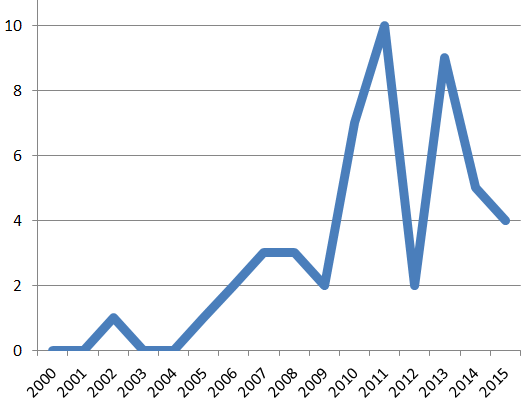
\includegraphics[scale=0.6]{PublicacionesAnuales.png}
  \end{center}
  \caption{Distribución de las publicaciones por años}
  \label{fig:PublicacionesAnuales}
\end{figure}

\subsection{Categorización del estudio}

Una vez revisados todos los artículos, se han extraído unas características o categorías comunes a la tipología de los trabajos. Todos los trabajos seleccionados hacen uso de algún tipo de software o metodología para evaluar algún tipo de competencia genérica. Sólo dos trabajos mencionan un enfoque como el que se propone en la introducción de este capítulo, es decir, aprovechando los registros de interacción de los estudiantes con el LMS como indicadores del desempeño de las competencias genéricas. Encontramos trabajos que se apoyan en la tecnología para el tratamiento o evaluación de las competencias, pero que terminan delegando parte de esta evaluación en el alumnado, ya sea mediante autoevaluación o evaluación entre iguales. Otros trabajos se basan en videojuegos o en las redes sociales para evaluar alguna competencia, mientras que otros desarrollan algún tipo de software o técnica. Finalmente hay algunos trabajos que simplemente detectan en su entorno la necesidad de la evaluación de las competencias de manera automática porque su forma de hacerlo les ocasiona una serie de problemas o desventajas con respecto a otro método que proponen o demandan. Además se han encontrado algunas revisiones sobre la literatura relacionadas que también serán tratadas aparte.  En la tabla \ref{tab:PublicacionesForum} se puede ver la distribución de las publicaciones. Algunos trabajos utilizan más de un método simultáneamente. %, apoyadas gráficamente en la figura  \ref{fig:PublicacionesForum}.

\begin{table}
  \begin{center}
  \begin{tabular}{| m{10cm} | c |}
    \hline
    CATEGORÍA & TRABAJOS\\
    \hline
    \hline 
    Peer and self-assessment & 18\\
    \hline
    Teacher assessment & 21\\
    \hline
    Questionaries & 16\\
    \hline
    Learning Analytics & 2\\
    \hline
  \end{tabular}
\end{center}
\caption{Distribución de publicaciones por tratamiento del problema}
\label{tab:PublicacionesForum}
\end{table} 

%\begin{figure}
%  \begin{center}
%    \includegraphics[scale=0.4]{cap3_pub_forum.png}
%  \end{center}
%  \caption{Distribución de publicaciones por tratamiento del problema}
%  \label{fig:PublicacionesForum}
%\end{figure}

En la figura \ref{fig:Burble} se muestra la clasificación de los trabajos según su ámbito y su tipo (lado izquierdo), y según su ámbito y su contribución (lado derecho). La evaluación de competencias genéricas mediante el uso de las nuevas tecnologías es un tema poco desarrollado. No sólo corroborado porque hay pocos trabajos, si no también a partir de esta figura. La mayoría de los trabajos son propuesta s(\emph{Proposal of solution}), experiencias (\emph{Experience papers}), validaciones (\emph{Validation research}) y evaluaciones de la investigación (\emph{Evaluation research}), mientras que trabajos de opinión(\emph{Opinion papers}) o filosóficos (\emph{Philosophical papers}), trabajos típicos de un tema de investigación de cierta madurez, casi no hay.

El tipo de contribución está más distribuído. Las contribuciones del tipo proceso (\emph{Process}) y modelo (\emph{Model}) son las que se dan con más frecuencia, la primera con cuestionarios (\emph{Questionnarie}), evaluación del profesores (\emph{Teacher assessment}) y autoevaluaciones o evaluaciones entre compañeros (\emph{Peer and self-assessment}), mientras que la segunda se da con más frecuencia con cuestionarios y evaluaciones del profesor. 

\pagestyle{empty}
\begin{landscape}
\begin{figure}[H]
  \begin{center}
    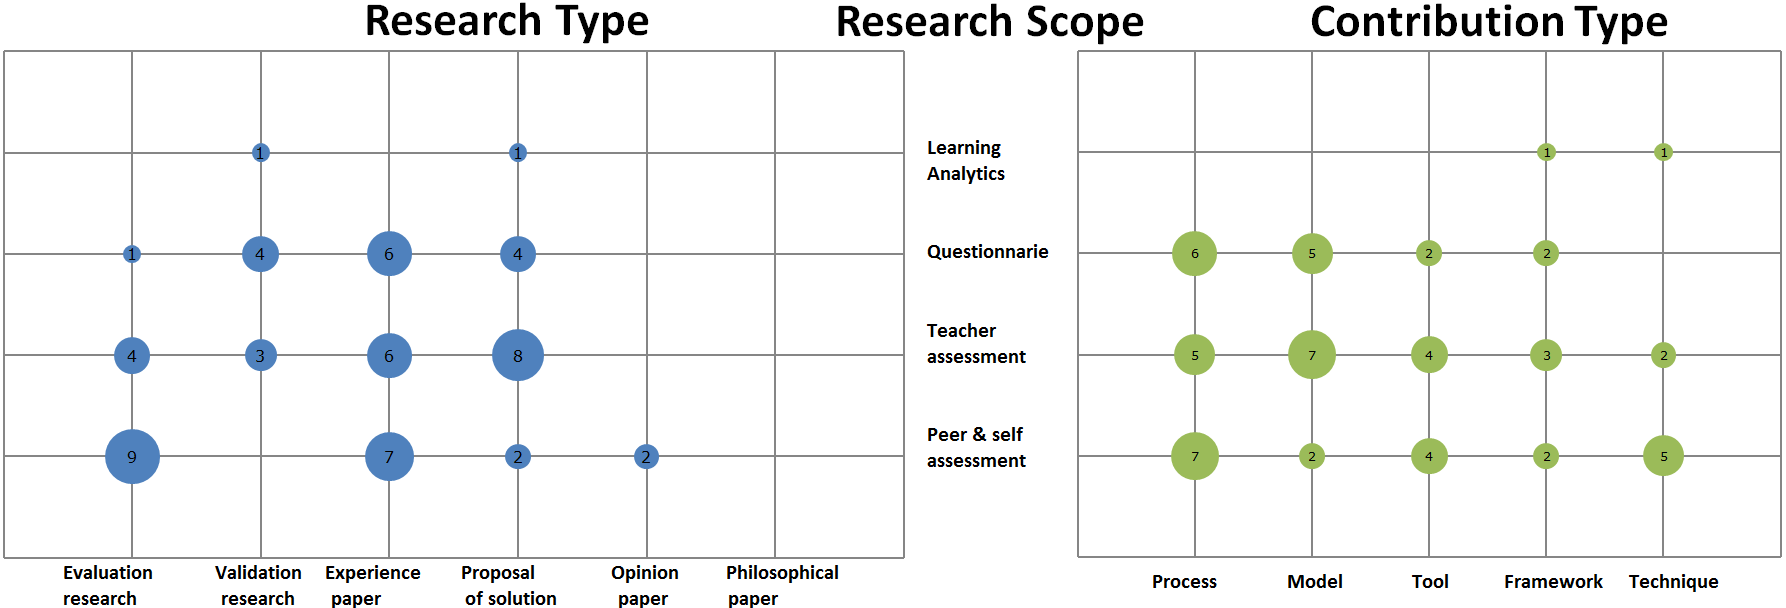
\includegraphics[scale=0.4]{Burbujas.png}
  \end{center}
  \caption{Ámbito de trabajos distribuidos según tipo de investigación y según tipo de contribución.}
  \label{fig:Burble}
\end{figure}
\end{landscape}
\pagestyle{fancy}

\subsection{Esquema de clasificación}

bla bla bla

\subsubsection{Peer and self-assessment}

La autoevaluación es un proceso en el que los estudiantes evaluan su propio trabajo, mientras que  en el proceso de evaluación entre iguales un estudiante evalúa el trabajo de otro u otros estudiantes. Esta práctica se emplea por un lado para ahorrar tiempo del profesorado, y por otro, para mejorar tanto el conocimiento en la materia del alumnado como sus habilidades metacognitivas. A menudo este tipo de evaluación se acompaña de algun tipo de rúbrica \cite{malehorn1994ten}.

Se han encontrado muchos trabajos en la literatura que utilizan este enfoque para evaluar competencias genéricas. De acuerdo a las preguntas de investigación de este trabajo únicamente se hanrecopilado aquellos trabajos que bajo este enfoque hagan uso de los ordenadores.

Se han encontrado varios trabajos que implementan una metodología de \emph{aprendizaje basado en problemas} (ABP o, del inglés, PBL, problem-based learning) para desarrollar competencias específicas y genéricas en sus estudiantes. En \cite{lasa2013problem} los profesores llevaron a cabo la evaluación del 90\% de las competencias utilizando la herramienta de rúbricas \emph{RubiStar}, mientras que los estudiantes mediante autoevaluación y evaluación entre iguales se encargaron del otro 10\%. En \cite{renau2010teaching} también se lleva a cabo una experiencia basada en una metodologia ABP para el desarrollo de la competencia en \emph{lengua extranjera} (inglés) en la que los estudiantes llevaban a cabo una autoevaluación de su nivel de adquisición de la competencia. En \cite{johnson2002encouraging} se muestran ejercicios para el desarrollo de competencias genéricas relacionados también con otra experiencia basada en una metodologia ABP y en unas presentaciones, siguiendo un enfoque de evaluaciones entre compañeros. En otro trabajo, vemos como los estudiantes después de haber realizado experiencias de videoconferencias en inglés, la competencia de \emph{inglés como lengua extranjera} junto con las competencias de \emph{trabajo en equipo} y \emph{comunicación oral} se evalúan en \cite{masip2013self} mediante auto y co-evaluación a través de Moodle.

El espíritu empresarial es considerado un factor fundamental para el desarrollo económico en todos los países del mundo \cite{DeXena2012educacion} y son muchos los trabajos que tratan de fomentar competencias genéricas relacionadas con las habilidades que un emprendedor ha de desempeñar. En \cite{chang2009international} se utiliza la herramienta Cycloid para el desarrollo de competencias en la gestión de proyectos y porteriormente se llevan a cabo autoevaluaciones de los propios estudiantes para valorar la adquisición de dichas competencias. En \cite{marquez2010have} se autoevalúan las competencias de \emph{iniciativa} y \emph{espíritu emprendedor}. También se autoevaluan competencias \emph{empresariales} en  \cite{achcaoucaou2014competence} mediante el uso de Tricuspoid. 

Un e-portfolio (del inglés \emph{electronic portfolio}, consiste en un conjunto de documentos, generalmente textos, archivos e imágenes, gestionados en un entorno web por un usuario. Se han recopilado trabajos donde los estudiantes trabajan con esta herramienta durante el curso y al final autoevalúan el desempeño de alguna competencia genérica. Por ejemplo, en \cite{arno2011promoting} se lleva a cabo una autoevaluación de la competencia del \emph{pensamiento crítico} tras haber trabajado en un e-portfolio. Mientras que en \emph{starcic2008sustaining} se utiliza también un e-portfolio para el desarrollo profesional de los estudiantes y se facilitan rubricas para la propia autoevaluación después de sus competencias genéricas.

En muchos trabajos la autoevaluación completa algún otro tipo de evaluación. En \cite{sevilla2012assessment} se utiliza plataforma online inGenio Tester para evaluar el nivel de adquisición de competencias en las modalidades de autoevaluación y evaluación por parte del profesor. En \cite{ficapal2015learning} se presenta un modelo que persigue el aprendizaje basado en equipos para la adquisición y evaluación de competencias genéricas en un contexto de e-learning. Los estudiantes trabajaban en grupo y evaluaban su desempeño en el \emph{trabajo en equipo} mediante una rúbrica. La calificación se completó con un cuestionario. En \cite{khamis2012measurement} también se trabajó y evaluó la competencia de \emph{trabajo en equipo}. Para ello los estudiates trabajaron en equipo y la evaluación tenía dos partes: por un lado los compañeros eran evaluados por otros compañeros (evaluación entre iguales) y por otro lado, también el profesor formaba parte de esta evaluación. En \cite{barbera2011assessment} se desarrollan y evalúan el desarrollo y desempeño de tres competencias genéricas en sus estudiantes: \emph{comunicación verbal}, \emph{comunicación escrita} y \emph{trabajo en equipo}. Este estudio propone una metodología basada en el modelo de tres niveles de evaluación de competencias utilizado por la Universidad de Deusto mediante diferentes herramientas utilizando tres tipos de evaluaciones: autoevaluación, evaluación entre iguales y evaluación del profesor.

Las herramientas 2.0 como wikis o blogs también se utilizan para medir el desempeño en competencias genéricas. En \cite{piedra2010measuring} se utilizan una serie de rúbricas para la autoevaluación de los estudiantes a partir de una serie de indicadores del desempeño de las competencias genéricas de la \emph{creatividad} y del \emph{trabajo colaborativo} a partir de su trabajo en herramientas de trabajo colaborativo. En \cite{mcloughlin2006beyond} se presentan una revisión de herramientas online para trabajar y evaluar competencas genéricas. Entre ellas también se mencionan herramientas colaborativas para la competencia del \emph{trabajo en equipo}.

Para la evaluación de la competencia de la capacidad \emph{autocrítica} se realizó una experiencia en \cite{pinto2011assessment}, dónde un conjunto de profesores de diferentes titulaciones establecieron actividades para los estudiantes. Estos estudiantes evaluaron su propio trabajo. Para medir el grado de competencia de los estudiantes se utilizó la diferencia de la nota entre la que recibieron los estudiantes por parte del profesor y la que ellos mismos se pusieron. En \cite{sin2007evaluating} también se realizó una experiencia donde tanto los propios estudiantes como los profesores evaluaban el desempeño de las competencias de la comunicación en contabilidad, tanto las \emph{habilidades para expresarse de manera escrita} como del \emph{pensamiento analítico}.

Aunque la autoevaluación y evaluación entre iguales son enfoques que quitan trabajo al docente, no todos son ventajas. Como se ha visto en algunos trabajos anteriores, este enfoque a menudo sólo se utiliza de manera complementaria a algún otro tipo de evaluación. Además, se puede dar el caso que la autoevaluación no se ajuste del todo a la realidad del desempeño del estudiante. Por ejemplo, en \cite{carreras2013promotion} hay notables diferencias entre las calificaciones que se auto-asignan los estudiantes en algunas competencias y las calificaciones que le asignaron los profesores en esas mismas competencias. En ese trabajo se promovió la adquisición de competencias genéricas desde un punto de vista interdisciplinar y se diseñaron herramientas especifícas para evaluar dichas habilidades. A la hora de evaluar, se realizaron tanto autoevaluaciones como evaluaciones del profesor. En esta experiencia se evaluaron cuatro competencias genéricas: \emph{capacidad de análisis},  \emph{habilidades de escritura}, \emph{responsabilidad} y \emph{capacidad de trabajo en equipo}. Cabe destacar discrepancias entre las calificaciones que se auto-asignan los estudiantes en las dos primeras competencias. En la \emph{capacidad de análisis} la discrepancia es de un 55,65\%, mientras que en las \emph{habilidades de escritura} de un 13,75\%.

\subsubsection{Teacher assessment}

En muchos casos la evaluación de competencias genéricas se realiza mediante un seguimiento continuo del trabajo del estudiante por parte del profesor. Este proceso es lo que se conoce como \emph{evaluación continua}. Esto permite ir introduciendo mejoras constantes en el proceso de aprendizaje, siendo éste el motivo por el que la evaluación continua se adopta como una estrategia de evaluación formativa más orientada al proceso de aprendizaje que a una valoración puntual. Actualmente, los expertos, influenciados por la \emph{Declaración de Bolonia}, consideran más apropiado desarrollar este tipo de sistemas de evaluación~\cite{garcia2005competencias}. 

En trabajos como los mostrados en \cite{martin2010new,prashar2010competence}, el profesorado sigue una metodología de evaluación continua para evaluar las competencias de \emph{trabajo en equipo} y \emph{comunicación oral y escrita}. Se establecen una serie de indicadores que les permiten monitorizar el progreso de los estudiantes. Una herramienta que se suele utilizar para hacer un seguimiento del trabajo de los estudiantes a lo largo del curso es el e-portfolio. En \cite{martin2013acquired,rodriguez2010portfolio,benlloch2007adapting} los profesores evalúan el desempeño de los estudiantes en las competencias de \emph{trabajo en equipo} y \emph{habilidades de comunicación} o \emph{solución de problemas}, entre otras. Para ello utilizan el e-portfolio, aunque en todos los casos combinan la evaluación del trabajo realizado por cada estudiante en el suyo junto con la calificaciones de otras actividades, exámenes y cuestionarios.

En \cite{yang2014fine} se define un modelo de itinerario de aprendizaje que soporta la evaluación de algunos conocimientos y competencias para describir el progreso de aprendizaje del estudiante. El modelo se define matemáticamente para poder formalmente definir las evaluaciones y para poder reutilizar las fórmulas. Aunque se reconoce las ventajas de un sistema que automatice este proceso, hasta el momento son los profesores los que evalúan a sus estudiantes en cada una de sus etapas. Además, muestran su reticencia a un sistema 100\% automático. Las competencias de \emph{comunicación} y \emph{escritura} se evalúan en este trabajo.

Uno de los problemas de la no automatización de los procesos de evaluación es la escalabilidad de algunos procesos de evaluación. En \cite{serrano2013hiperion} se diseña \emph{Hiperion}, una sistema de recomendación que ayuda a diseñar actividades adaptadas a cada estudiante para mejorar sus competencias. En el estudio de caso mostrado en este trabajo, los profesores evaluaban las competencias de los estudiantes manualmente y después aplicaban Hiperion. La principal desventaja de la herramienta es el tiempo que el profesor ha de dedicar para asignar los diferentes logros y el peso de cada nota para cada competencia en las actividades. En \cite{ward2011developing} se desarrollan una serie de módulos para Moodle para el desarrollo de competencias empresariales. Los alumnos realizan una serie de actividades para cada módulo y el profesor evalúa mediante conferencia via Skype si cada estudiante sabe lo que ha respondido. En \cite{lacuesta2009active} se utiliza una metodología ABP, dónde se realiza una evaluación individualizada de cada estudiante y de cada grupo de estudiantes. El autor considera que el esfuerzo necesario y carga de trabajo para cada profesor sólo es un poco mayor al habitual. En este trabajo se evaluan competencias como la \emph{capacidad critica}, \emph{trabajo en equipo}, \emph{planificación}, \emph{comunicación}, etc. Para minimizar el esfuerzo están las rúbricas, utilizadas en \cite{casan2015developing}, donde el docente se encarga mediante su uso de la evaluación en las habilidades de \emph{comunicación escrita} del alumnado.

\subsubsection{Questionnarie}

En \cite{lumsden2005assessment} se muestra la herramienta PQA (Personal Quality Assessment). Esta herramienta de evaluación contiene diversos test para la evaluación de la competencia genérica del \emph{razonamiento} y del {comportamiento ético} en el ámbito médico.

Trabajos: \cite{vizcarro2013assessment}, \cite{ruizacarate2013soft}, \cite{barbera2011design}, \cite{so2011mapping}, \cite{badcock2010developing}, \cite{aziz2007appraisal}, \cite{rashid2008engineering}, \cite{a2007outcome}, \cite{albergaria2011critical}, \cite{park2006moral}, \cite{andre2011formal}, \cite{martinez2014teamwork}, \cite{fernandez2011experience}.

\subsubsection{Learning Analytics}


% JUEGOS SERIOS BASADOS EN INDICADORES: ¿LOS SACO DE LA?

En \cite{guenaga2013serious} se utilizan los juegos serios para el desarrollo de las competencias de \emph{emprendimiento} y \emph{solución de problemas}. Se definieron una serie de indicadores para alcanzar  que se plasmaron en un juego que permite al estudiante conocer su nivel de adquisición en dichas competencias.

En \cite{bedek2011behavioral} también se utilizan los juegos serios para el desarrollo y evaluación de competencias genéricas. Se basa en un modelo donde para casa competencia se identifican subcompetencias más específicas, lo que facilita el proceso de definición de indicadores.

Trabajos: \cite{fidalgo:2015} and \cite{rayon2014web}

\section{Respuestas}


%\chapter{Trabajo en curso y futuro}

\section{Conclusiones}

\pagestyle{empty}
\begin{landscape}
\begin{center}
\begin{longtable}{| m{2.5cm} | m{9cm} | m{4cm} | m{2.5cm} | m{3.5cm} |}
    \hline
    REF & TÍTULO & TIPO DE INVESTIGACIÓN & TIPO DE CONTRIBUCIÓN & ÁMBITO DE LA INVESTIGACIÓN \\
    \hline
    \hline 
    \cite{yang2014fine} & A Fine-Grained Outcome-Based Learning Path Model & proposal of solution & model & Teacher assessment \\
    \hline
    \cite{rayon2014web} & A web platform for the assessment of competences in Mobile Learning Contexts & validation research & framework & Learning analytics \\
    \hline
    \cite{martin2013acquired} & Acquired Skills With The Implementation Of New Evaluation Methods At University Rey Juan Carlos & experience paper & model & Teacher assessment \\
    \hline
    \cite{lacuesta2009active} & Active learning through problem based learning methodology in engineering education & experience paper & process & Teacher assessment \\
    \hline
    \cite{benlloch2007adapting} & Adapting teaching and assessment strategies to enhance competence-based learning in the framework of the european convergence process & proposal of solution & process & Teacher assessment / Questionnarie \\
    \hline
    \cite{aziz2007appraisal} & Appraisal of Course Learning Outcomes using Rasch Measurement: A Case Study in Information Technology Education & proposal of solution & model & Questionnarie / Teacher assessment \\
    \hline
    \cite{sevilla2012assessment} & Assessment of competences in designing online preparatory materials for the Cambridge First Certificate in English examination & evaluation research & technique & Peer and self-assessment / Teacher assessment \\
    \hline
    \cite{lumsden2005assessment} & Assessment of personal qualities in relation to admission to medical school & evaluation research & framework & Questionnarie \\
    \hline
    \cite{vizcarro2013assessment} & Assessment of problem solving in computing studies & experience paper & process & Questionnarie \\
    \hline
    \cite{pinto2011assessment} & Assessment Of Self-Criticism Capacity Competence In Higher Education Students: Outcome Oriented Education & experience paper & process & Peer and self-assessment \\
    \hline
    \cite{barbera2011assessment} & Assessment Tools For The Evaluation Of Generic Skills Development In Students Of Business Management & proposal of solution & model & Teacher assessment \\
    \hline
    \cite{mcloughlin2006beyond} & Beyond marks and measurement: Developing dynamic and authentic forms of e-assessment & opinion paper & technique & Peer and self-assessment \\
    \hline
    \cite{achcaoucaou2014competence} & Competence Assessment in Higher Education: A Dynamic Approach & proposal of solution & tool & Peer and self-assessment \\
    \hline
    \cite{prashar2010competence} & Competence Based Teaching And Evaluation In The General Chemistry Course Of The University Rey Juan Carlos & experience paper & framework & Teacher assessment \\
    \hline
    \cite{strijbos2015criteria} & Criteria and standards of generic competences at bachelor degree level: A review study & evaluation research & process & Pending \\
    \hline
    \cite{albergaria2011critical} & Critical Thinking, Questioning and Creativity as Components of Intelligence & proposal of solution & process & Questionnarie \\
    \hline
    \cite{barbera2011design} & "Design And Results Of Collaborative Project-Based Learning In The Subject Commercial Management"" In Industrial Organization Engineering""" & experience paper & framework & Questionnarie \\
    \hline
    \cite{ward2011developing} & Developing entrepreneurial accounting and finance competency using the ELLEIEC Virtual Centre for Enterprise & experience paper & tool & Teacher assessment \\
    \hline
    \cite{badcock2010developing} & Developing generic skills through university study: a study of arts, science and engineering in Australia & experience paper & model & Questionnarie \\
    \hline
    \cite{casan2015developing} & Developing Writing Skills in The Classroom: A Corpus-based Analysis of Multi-Genre Structures & proposal of solution & model & Teacher assessment \\
    \hline
    \cite{ficapal2015learning} & e-Learning and Team-based Learning. Practical Experience in Virtual Teams & experience paper & framework & Peer and self-assessment / Questionnarie \\
    \hline
    \cite{johnson2002encouraging} & Encouraging generic skills in science courses & proposal of solution & process & Peer and self-assessment / Teacher assessment \\
    \hline
    \cite{rashid2008engineering} & Engineering Students Performance Evaluation of Generic Skills Measurement: ESPEGS Model & validation research & model & Questionnarie / Teacher assessment \\
    \hline
    \cite{rodriguez2010portfolio} & e-Portfolio: A tool to assess university students' skills & evaluation research & tool & Teacher assessment \\
    \hline
    \cite{sin2007evaluating} & Evaluating a method of integrating generic skills with accounting content based on a functional theory of meaning & evaluation research & process & Peer and self-assessment / Teacher assessment \\
    \hline
    \cite{andre2011formal} & Formal model for assigning human resources to teams in software projects & validation research & model & Questionnarie \\
    \hline
    \cite{bedek2011behavioral} & From Behavioral Indicators to Contextualized Competence Assessment & proposal of solution & framework & Teacher assessment \\
    \hline
    \cite{oliver2013graduate} & Graduate attributes as a focus for institution-wide curriculum renewal: innovations and challenges & opinion paper & model & Peer and self-assessment \\
    \hline
    \cite{marquez2010have} & Have Our Future Entrepreneurs An Ethical Commitment? & evaluation research & process & Peer and self-assessment \\
    \hline
    \cite{serrano2013hiperion} & Hiperion: A fuzzy approach for recommending educational activities based on the acquisition of competences & proposal of solution & tool & Teacher assessment \\
    \hline
    \cite{chang2009international} & International creative tension study of university students in South Korea and Finland & evaluation research & tool & Peer and self-assessment \\
    \hline
    \cite{} & Making Explicit and Reinforcing Horizontal Competences in an Electronic Engineering Degree & validation research & process & Teacher assessment \\
    \hline
    \cite{so2011mapping} & Mapping The Impact On Holistic Development: A Study Of The Relationship & proposal of solution & process & Questionnarie \\
    \hline
    \cite{khamis2012measurement} & Measurement of Students' Performance Level in a Group Project by using Peer Review and Lecturer Assessment & experience paper & technique & Peer and self-assessment / Teacher assessment \\
    \hline
    \cite{piedra2010measuring} & Measuring collaboration and creativity skills through rubrics: Experience from UTPL collaborative social networks course & evaluation research & process & Peer and self-assessment \\
    \hline
    \cite{park2006moral} & Moral competence and character strengths among adolescents: The development and validation of the Values in Action Inventory of Strengths for Youth & validation research & tool & Questionnarie \\
    \hline
    \cite{martin2010new} & New Methodologies In The Teaching And Evaluation Of The Competences “Teamwork” And “Oral And Written Communication” In The Civil Law Course Of The University Rey Juan Carlos & experience paper & framework & Teacher assessment \\
    \hline
    \cite{a2007outcome} & Outcome based education performance assessment: A computational model to measure electrical engineering subjects learning outcomes & evaluation research & model & Questionnarie /Teacher assessment \\
    \hline
    \cite{lasa2013problem} & Problem Based Learning Implementation In The Degree Of Human Nutrition And Dietetics & experience paper & technique & Peer and self-assessment / Teacher assessment \\
    \hline
    \cite{arno2011promoting} & Promoting reflection on science, technology, and society among engineering students through an EAP online learning environment & evaluation research & tool & Peer and self-assessment \\
    \hline
    \cite{masip2013self} & Self-video recording for the integration and assessment of generic competencies & experience paper & technique & Peer and self-assessment \\
    \hline
    \cite{guenaga2013serious} & Serious Games for the Development of Employment Oriented Competences & validation research & tool & Teacher assessment \\
    \hline
    \cite{ruizacarate2013soft} & Soft Skills: A Comparative Analysis Between Online and Classroom Teaching & experience paper & process & Questionnarie \\
    \hline
    \cite{starcic2008sustaining} & Sustaining Teacher's Professional Development and Training through Web-Based Communities of Practice & evaluation research & tool & Peer and self-assessment \\
    \hline
    \cite{renau2010teaching} & Teaching And Learning Through Projects Using The ICT: Practice Of The English Writing Through Business Documents & experience paper & process & Peer and self-assessment \\
    \hline
    \cite{martinez2014teamwork} & Teamwork competence and academic motivation in computer science engineering studies & validation research & process & Questionnarie \\
    \hline
    \cite{fernandez2011experience} & The experience of implementing a communication skills assessment in the first year course for undergraduate computing engineering students: A tool for further development of an international curriculum & experience paper & tool & Questionnarie \\
    \hline
    \cite{carreras2013promotion} & The promotion and assessment of generic skills from interdisciplinary teaching teams & experience paper & process & Peer and self-assessment / Teacher assessment \\
    \hline
    \cite{fidalgo:2015} & Using Learning Analytics to improve teamwork assessment & proposal of solution & technique & Learning analytics \\
    \hline
\caption{Distribución de publicaciones por tratamiento del problema}
\label{tab:ListadoTrabajos}
\end{longtable}
\end{center}
\end{landscape}

\pagestyle{fancy}


% ----------------------------------------------------------------------

	

%: ----------------------- problemas encontrados ------------------------
% introduction

% this file is called up by thesis.tex
% content in this file will be fed into the main document

%: ----------------------- introduction file header -----------------------
%\begin{savequote}[50mm]
%Now this is not the end. It is not even the beginning of the end. But it is, perhaps, the end of the beginning. 
%\qauthor{Winston Churchill}
%\end{savequote}

\chapter{Resumen de problemas encontrados}
\label{cha:Problemas}

% the code below specifies where the figures are stored
\ifpdf
    \graphicspath{{3_problemas/figures/PNG/}{3_problemas/figures/PDF/}{3_problemas/figures/}}
\else
    \graphicspath{{3_problemas/figures/EPS/}{3_problemas/figures/}}
\fi


%------------------------------------------------------------------------- 

En el capítulo anterior se ha realizado una revisión de la literatura para responder a diversas cuestiones sobre la evaluación de competencias genéricas mediante el uso de métodos y herramientas informáticas, así como de cuáles son esos métodos y si usan los registros de actividad de los entornos virtuales de aprendizaje. A raíz de esta revisión han aflorado varios problemas para cada tipo de evaluación encontrado que son resumidos a continuación. También se indican en este capítulo los requisitos que deberá tener el método a desarrollar a tenor de los problemas anteriores.

\section{Problemas encontrados}

La explicación de los problemas encontrados se organiza según los tipos de evaluación de los trabajos (asistida y semiautomática). Para cada uno de ellos se resumirán los problemas encontrados.

\subsection{Evaluación asistida} % de los estudiantes es la de dar

En este tipo de evaluación la herramienta informática da soporte al usuario para que éste lleve a cabo la evaluación. Para ello le proporciona el formato para introducir datos (notas, indicadores, respuestas a preguntas, etc.). Estos datos podrán ser introducidos por los alumnos (autoevaluación o evaluación entre iguales) o por el docente (evaluación del docente).

\subsection*{Autoevaluación o evaluación entre iguales} \label{cha:pro-sec:aut}

La autoevaluación es un proceso en el que los estudiantes evalúan su propio trabajo, mientras que  en el proceso de evaluación entre iguales un estudiante evalúa el trabajo de otros estudiantes. La mayor virtud de este tipo de evaluación es que mejora tanto el conocimiento en la materia del alumnado como sus habilidades metacognitivas. Otra ventaja de esta evaluación es que ahorra parte del trabajo del docente.

A continuación se van a describir los problemas encontrados por los autores a la hora de realizar una evaluación de una o varias competencias genéricas con un enfoque de autoevaluación o evaluación entre iguales.

\paragraph*{Subjetividad}
En ocasiones las calificaciones que asignan los estudiantes no se ajustan a la que recibirían del docente, habiendo diferencias notables entre las calificaciones que asignan diferentes estudiantes o el docente a un mismo trabajo. Este tipo de evaluaciones suelen ir acompañados de rúbricas para guiar el proceso de evaluación~\cite{malehorn1994ten}. Sin embargo, no todas las competencias a evaluar y los aspectos derivados a tener en cuenta pueden ser recogidos en una rúbrica. Si a esto unimos la falta de madurez que pueden tener los estudiantes o una interpretación diferente que estos realicen de los criterios de evaluación, las diferencias entre la calificación que el docente daría a un trabajo y la que darían sus estudiantes podrían ser importantes~\cite{carreras2013promotion}. %Se han encontrado casos relacionados con competencias como la \emph{capacidad de análisis} o las \emph{habilidades de escritura}. 

\paragraph*{Escalabilidad}
Se dice que un proceso de evaluación sufre problemas de escalabilidad cuando el número de trabajos a evaluar crece y el evaluador no es capaz de abarcar este crecimiento. A priori podría pensarse que la autoevaluación o evaluación entre iguales son estrategias que ahorran trabajo al docente, ya que son los estudiantes los que se encargan de la evaluación. Sin embargo, más que ahorrar trabajo, podría decirse que el docente adopta otro papel, ya que de evaluar trabajos pasa a moderar o revisar las evaluaciones de los estudiantes~\cite{bostock2000student}. Además, el tiempo que debiera dedicar el docente a revisar las evaluaciones de los trabajos puede ser en muchos casos superior al tiempo que dedicaría a evaluar los trabajos.

Por ejemplo, supongamos que un docente tiene un número dado de estudiantes en clase ($n$) y el tiempo de evaluación que le requiere el trabajo realizado por cada estudiante es $t_{eval}$. Evaluar el trabajo de estos estudiantes le tomará un tiempo de $T = n*t_{eval}$. Aplicando el principio de invarianza multiplicativa esta es una actividad desde un punto de vista temporal de orden $n$ ($O(n)$). 

Si optamos por una estrategia de evaluación entre iguales en la que cada estudiante evalúa a un número determinado de compañeros ($k$) y el docente considera revisar las evaluaciones realizadas por sus estudiantes, teniendo en cuenta que la revisión de cada evaluación le requiere un tiempo $t_{rev}$, este proceso tendría un coste de $T = k*n*t_{rev}$.

Dependiendo del número de evaluaciones que tenga que realizar cada estudiante nos encontraremos en diversos casos:
\begin{itemize}
	\item Mejor caso: cada estudiante sólo evalúa a un único compañero ($k=1$). En este caso $T = n*t_{rev}$. Por el principio de invarianza multiplicativa este proceso sería también de ($O(n)$).
	\item Peor caso: cada estudiante evalúa a todos sus compañeros ($k = n - 1$). En este caso $T = n*(n-1)*t_{rev} = n^{2}*t_{rev} - n*t_{rev}$. Aplicando el principio de invarianza multiplicativa y la del máximo de dos órdenes queda que este caso es de orden cuadrático ($O(n^{2})$).
\end{itemize}

Es difícil establecer un caso promedio o general, pero si un docente fijase que cada estudiante tuviese que evaluar a la mitad de sus compañeros ($n/2$) o a un tercio ($n/3$), el orden del proceso, aplicando el principio de invarianza multiplicativa, seguiría siendo cuadrático ($O(n^{2})$).

%Dependiendo de la relación que haya entre $t_{eval}$ y $t_{rev}$ el docente habrá ganado o no algo de tiempo. Si un docente tarda en revisar una evaluación de un trabajo un 60\percentage{ }del tiempo que tarda en corregir un trabajo del mismo tipo ($t_{rev} = 0.6*t_{eval}$), el proceso descrito anteriormente le llevará un 20\percentage{ }más del tiempo del que le llevaba el proceso normal.
% Obviamente, si no se revisan las evaluaciones entre iguales sí se ahorra tiempo, pero no es lo habitual.

Por tanto, en el mejor caso, ambas estrategias no difieren en su implementación en más de alguna constante multiplicativa, siendo ambas estrategias de orden n ($O(n)$). Pero en el caso general, el orden del proceso de revisión de las autoevaluaciones realizadas por los estudiantes es cuadrático ($O(n^{2})$), mayor que el orden de tiempo que conlleva la evaluación del docente de los trabajos ($O(n)$). Por lo que puede afirmarse que este enfoque no resuelve el problema de la escalabilidad.

En algunos de los trabajos revisados, puede verse como tras la evaluación realizada por los estudiantes, los docentes han de revisar dichas evaluaciones~\cite{lasa2013problem,sevilla2012assessment}. Los autores indican la sobrecarga de trabajo que ello les supuse, quedando por tanto ilustrado lo mencionado en el análisis anterior. %Más sentido tiene aún esta revisión del profesor si tenemos en cuenta problemas como el descrito anteriormente, en los que las calificaciones de los estudiantes puede que no se ajusten a la realidad.

\subsection*{Evaluación del docente}

En esta sección se recogen problemas asociados a los trabajos en los que la evaluación la realiza directamente el docente apoyándose en la tecnología.

\paragraph*{Escalabilidad}
La escalabilidad vuelve a ser el problema más mencionado en este tipo de evaluación. Los autores de los trabajos comparten experiencias en las que evaluaron competencias genéricas, pero indican que la carga de trabajo les resultó excesiva~\cite{serrano2013hiperion,lacuesta2009active} e incluso uno de ellos descarta repetir la experiencia en los siguientes cursos debido al sobresfuerzo que le supuso~\cite{benlloch2007adapting}. Podemos deducir, por tanto, que si en ocasiones los docentes tienen tiempo ajustado para lograr los objetivos curriculares específicos de la materia que tienen que impartir y las evaluaciones que tienen que realizar, más difícil será lograr dichos objetivos si tienen que diseñar tareas adicionales para que los alumnos desempeñen competencias genéricas y después evaluarlas.

\subsection{Evaluación semiautomática}

En esta sección se recogen problemas asociados a trabajos que utilizan herramientas de evaluación semiautomática. Estas herramientas ayudan al docente en la evaluación proporcionándole de manera automática calificaciones o indicadores que éste puede usar para la evaluación de sus estudiantes. La intervención del docente en estas herramientas consiste en configuraciones iniciales de parámetros del curso o la evaluación.

La automatización de este proceso de evaluación solventa el problema de escalabilidad mencionado en los enfoques anteriores. Pero se encuentran otros problemas que serán descritos a continuación.


\paragraph*{Propósito específico}
Los recursos con los que cuentan los docentes están enfocados o fueron creados para un propósito específico. Dentro de los trabajos seleccionados esto ocurre principalmente con los juegos serios, que son diseñados para un propósito principal distinto del de la pura diversión y que generalmente están ligados a competencias específicas de las materias que se imparten en el contexto para el que fueron diseñados~\cite{bedek2011behavioral,guenaga2013serious}. Además, el desarrollo de un juego para evaluar las competencias concretas de un curso no es una tarea al alcance de cualquier docente. Pero este caso será tratado en el siguiente punto.


\paragraph*{Recursos limitados / Coste elevado}
Hay un trabajo que implementa un test psicológico de corrección automática para la evaluación de ciertas competencias genéricas. El diseño de un test de este tipo requiere personal cualificado en psicología, algo que obviamente no tienen todos los docentes. Además, para la experiencia que se encontró en la literatura fue necesario contar con un equipo de expertos que mediante el método Delphi definieron el test, algo con lo que tampoco suelen contar la mayoría de los docentes~\cite{andre2011formal}.

En los juegos serios ocurre lo mismo, un docente puede considerar cómo sería un videojuego para que el alumno aplique ciertas competencias genéricas y él después pueda evaluarle en dichas competencias, pero desarrollar un videojuego no es una tarea sencilla al alcance de cualquier docente.

\paragraph*{Validez de los indicadores}
Por último se han encontrado con un conjunto de trabajos que se basan en el \emph{learning analytics} para evaluar competencias genéricas. Para ello obtienen información de los registros de aprendizaje que utilizan como indicadores asociados a diferentes competencias genéricas~\cite{fidalgo:2015,rayon2014web}. El problema es que los indicadores son fijos, y lo que para un docente puede ser un indicador válido de la competencia de liderazgo, para otro puede no serlo. Por ello, se echa en falta un mecanismo para que sea el propio docente el que seleccione los indicadores que necesita, descarte los que no le sean útiles y los combine hasta obtener el indicador que sea válido para su caso. Es decir, lo que sería deseable es que hubiera un método para que el docente pueda diseñar sus propias evaluaciones en base a estos indicadores.

\section{Requisitos} \label{pro:requisitos}

Antes de comenzar con el desarrollo del método hay que enumerar los requisitos que éste deberá satisfacer para resolver los problemas mencionados en la sección anterior. Los requisitos son los que se detallan a continuación.

\paragraph*{1. Indicadores objetivos}

Los indicadores utilizados para medir el desempeño de los estudiantes deben ser objetivos. No ha lugar a consideraciones personales o interpretaciones inexactas de rúbricas como ocurre en la autoevaluación o evaluación entre iguales, donde dos evaluaciones de un mismo trabajo realizadas por personas diferentes pueden tener calificaciones diferentes. 

\paragraph*{2. Evaluación escalable}

El método para la evaluación de competencias genéricas deberá ser escalable, de manera que un crecimiento en el número de actividades a evaluar no le suponga un esfuerzo al docente que no pueda abordar. El método deberá estar alineado con las actividades de aprendizaje para que el docente pueda consultar los indicadores con una simple petición a la herramienta.

\paragraph*{3. Propósito general}

El método no debe estar orientado a una competencia específica ni genérica concreta. Es el docente quien diseña sus actividades en el entorno virtual de aprendizaje y el que luego obtiene los indicadores para utilizarlos en la evaluación de la competencia que considere que los estudiantes han desempeñado en dicha tarea (y que queda reflejada en los indicadores). 

\paragraph*{4. Accesibilidad}

No deberá ser un requisito que el docente tenga un perfil informático u otro específico para poder realizar las peticiones de los indicadores, ni que contrate a un equipo de expertos para obtener los indicadores. La interfaz en la que se implementará el método debe ser usable y sencilla para que los docentes puedan utilizarla sin requerirles conocimientos de programación, y los formatos a los que se exporte la información serán figuras y documentos en formatos transportables a cualquier hoja de cálculo.

\paragraph*{5. Diseño de evaluaciones}

El método debe poner a disposición del docente los mecanismos necesarios para que éste pueda diseñar sus propios indicadores a partir de los datos objetivos de la actividad de los estudiantes. En el estado del arte nos encontramos con trabajos que obtenían sus evaluaciones a partir de los indicadores del entorno virtual de aprendizaje, pero éstos eran fijos. Es decir, cada competencia se evaluaba con un indicador dado. Pero podía ocurrir que el docente no utilizase las actividades del entorno virtual que proporcionaban dichos indicadores o que plantease las actividades con un enfoque diferente al que realmente tienen. Por ejemplo, uno de los puntos fuertes de un wiki es que favorecen el trabajo colaborativo, y podríamos encontrar herramientas que nos ayuden a valorar el trabajo en equipo de los estudiantes que participan en una página de un wiki mediante indicadores del trabajo colaborativo. Si un docente plantea actividades en el wiki de manera que cada estudiante trabaje individualmente en una página, podrá valorar otras competencias, pero no el trabajo en equipo. Con este método el docente debe ser quien diseñe sus indicadores, y por tanto, sus evaluaciones a partir de los registros de las actividades de aprendizaje.

% ----------------------------------------------------------------------




%: ----------------------- overall methodology ------------------------
% introduction

% this file is called up by thesis.tex
% content in this file will be fed into the main document

%: ----------------------- introduction file header -----------------------
\begin{savequote}[50mm]
Historical methodology, as I see it, is a product of common sense applied to circumstances. 
\qauthor{Samuel E. Morison}
\end{savequote}


\chapter{Método para la evaluación de competencias genéricas}
\label{cha:Overall methodology}

% the code below specifies where the figures are stored
\ifpdf
    \graphicspath{{4_overall_methodology/figures/PNG/}{4_overall_methodology/figures/PDF/}{4_overall_methodology/figures/}}
\else
    \graphicspath{{4_overall_methodology/figures/EPS/}{4_overall_methodology/figures/}}
\fi

%------------------------------------------------------------------------- 

En este capítulo se propone un método para la evaluación de competencias genéricas de los estudiantes basado en el diseño de evaluaciones a partir de la actividad de estos en los entornos de aprendizaje. Se describe el método, sus características, los requisitos que el método ha de satisfacer y se introduce el tipo de herramienta que se empleará para su implementación.

\section{Introducción}

En esta tesis se propone un método de evaluación de competencias genéricas basado en el diseño de evaluaciones (DBA, del inglés, \emph{design-based assessment}) y que tiene su origen en la investigación basada en el diseño (DBR). DBA es un método de evaluación de competencias genéricas que se basa en indicadores de la actividad generada por los estudiantes en los entornos de aprendizaje virtual. Los profesores podrán diseñar evaluaciones utilizando estos indicadores y podrán utilizar estas evaluaciones como evidencias del desempeño de competencias genéricas. Estas evaluaciones podrán ser refinadas por el propio profesor hasta llegar a unas evidencias que le sean válidas. También podrán ser utilizadas y modificadas por otros profesores que busquen adaptarlo a su contexto local o a las competencias que ellos quieren realizar. 

Se podría decir que hoy en día los entornos virtuales constituyen una pieza fundamental en cualquier contexto en el que se impartan cursos. Mientras que en los cursos virtuales, los VLEs son el único entorno de trabajo posible, en los cursos presenciales o mixtos, tantos los VLEs como otras herramientas virtuales actúan como soporte virtual de las clases, proporcionando multitud de actividades de aprendizaje. 

En el VLE por ejemplo, los estudiantes pasan a diario por sus páginas. Por un lado, habrá estudiantes que accedan al VLE cada día a consultar novedades, participar en foros, subir tareas o descargar apuntes, mientras que por otro lado, habrá estudiantes que entren sólo de manera puntual, ya sea porque tienen un examen o porque tienen que subir una tarea. Todas las acciones de los estudiantes quedan almacenadas en el registro de las actividades de aprendizaje, y estos registros podrían ser analizados para comprender el proceso de aprendizaje que se está desarrollando mediante \emph{learning analytics}, contexto en el que sitúa el método DBA.

% Revisar párrafo anterior sobre el contexto de learning analytics

\section{Método: design-based assessment (DBA)}

\subsection{Contexto}

Los estudiantes comienzan a dejar constancia de su actividad en los entornos virtuales desde el momento en que acceden al entorno. El registro del sistema lo almacena todo, tanto la participación activa del estudiante, escribiendo y respondiendo mensajes en los foros o enviando actividades, como la participación pasiva, cuando simplemente se lee una página, se leen los mensajes del foro o se descargan los apuntes. 

Los programas de las asignaturas incluyen las competencias genéricas de las que los estudiantes deben ser evaluados. Los profesores pueden plantear actividades en los entornos virtuales con la intención no sólo de evaluar ciertas habilidades de los estudiantes, sino también de provocar comportamientos en los estudiantes y ver cómo afrontan ciertas situaciones. Pueden encontrarse patrones de comportamiento en la manera en que los estudiantes abordan ciertas tareas y estos comportamientos podrían ser interpretados como un indicador del desempeño de alguna competencia genérica.

Para evaluar una competencia genérica dada, el profesor podrá diseñar una evaluación a partir de la información relativa a los registros de los entornos de aprendizaje. Aquí comienza un \emph{ciclo de contraste de hipótesis}. 

%Ese diseño será procesado por el sistema que implementa el método y que terminará devolviendo la información al profesor. El resultado de aplicar el diseño será un indicador que el profesor podrá utilizar para la evaluación de la competencia genérica.


%También se puede dar el caso de que el profesor considere que el indicador no es válido para la evaluación de la competencia genérica. También puede que aunque le sea válido pero considere que un rediseño del mismo le permitirá afinar más en cuánto al objetivo de evaluación de competencia genérica que se marcó. El profesor podría diseñar una nueva evaluación a partir de la información contenida en el registro y así sucesivamente hasta que los resultados satisfagan su hipótesis, momento en el que termina el  \emph{ciclo de contraste de hipótesis}.


\subsection{Descripción del método}

El método DBA es iterativo, ya que permite al docente rediseñar y contrastar hipótesis y resultados hasta confirmar la hipótesis, o por el contrario, descartarla y enunciar una nueva. Podemos decir que el método se integra en un \emph{ciclo de contraste de hipótesis}. Este ciclo consta de una serie de pasos que se muestran en la figura~\ref{fig:CCHDiagram} y se explican a continuación:

\begin{figure}
  \begin{center}
    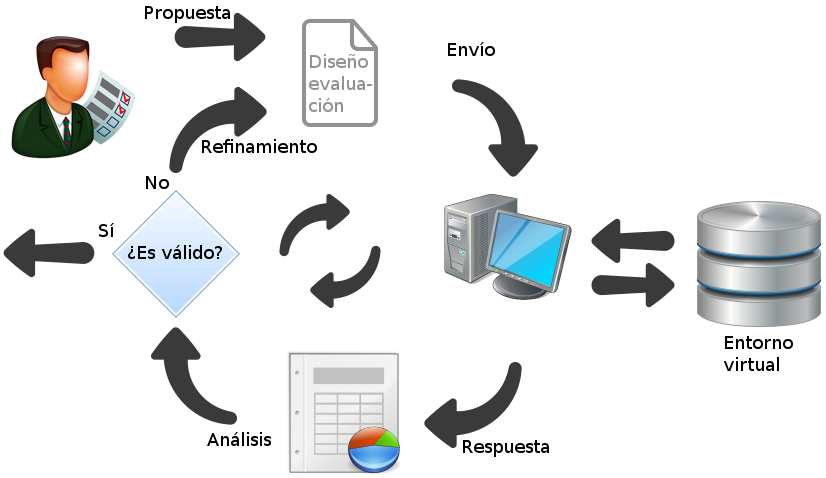
\includegraphics[scale=0.45]{CCHDiagram.png}
  \end{center}
  \caption{Diagrama del ciclo de contraste de hipótesis}
  \label{fig:CCHDiagram}
\end{figure}

\begin{enumerate}
\item \emph{Hipótesis inicial}: el profesor formula una hipótesis para la utilización de algún tipo de información de la actividad de los estudiantes en el entorno virtual para la evaluación de alguna competencia genérica (a). Por ejemplo, se considerará que un estudiante tiene un desempeño correcto de la competencia genérica de planificación y gestión del tiempo si entrega las tareas programadas por el profesor en el VLE con anterioridad a la fecha fijada para las mismas.
\item \emph{Diseño y formulación de evaluación}: el profesor diseñará un indicador para evaluar la competencia a partir de la información del registro y la implementará en la herramienta utilizada para extraer la información (b). Por ejemplo, podríamos considerar partiendo de la hipótesis anterior que un estudiante tendrá un desempeño alto en la competencia de planificación y gestión del tiempo si de las 10 tareas programadas durante el semestre al menos 9 fueron entregadas antes de la fecha fijada para las mismas, un desempeño medio si entregó entre 7 y 8 tareas antes de la fecha fijada y un desempeño bajo si entregó 6 o menos tareas antes de la fecha fijada.
\item \emph{Petición de datos}: Se enviará la petición de datos al sistema encargado de recuperar la información (c). Las herramientas y su funcionamiento serán explicadas más adelante en la sección~\ref{sec:tools}.
\item \emph{Validación de resultados}: la herramienta pondrá a disposición del profesor los indicadores requeridos (d). El profesor los analizará (e) y evaluará si son válidos para el propósito que fueron diseñados (f), si necesitan ser refinados o si hay que descartarlos. En este caso, podrá volver al segundo punto y rediseñar una nueva evaluación (g).
\end{enumerate}

\section{Características, requisitos y herramienta}

El método DBA para la evaluación de competencias genéricas es un método DBR. Aunque desde el punto de vista del estudiante y considerando la clasificación de métodos de evaluación mostrada en la sección~\ref{sec:methods} diríamos que es un método \emph{evaluación formativo}, ya que permite mejorar el aprendizaje mientras este tiene lugar proporcionando información de manera sistemática y continua. Sin embargo, lo consideramos un método DBR ya que no mejora únicamente la acción del alumno, sino que también es un método de investigación que mejora la acción del profesor.

Mientras que con respecto a la clasificación de técnicas de evaluación mostrada en la sección~\ref{sec:techniques}, la técnica empleada en este método es la de obtención de \emph{indicadores del trabajo en actividades de aprendizaje}.

\subsection{Características}

En el apartado~\ref{sec:dbr} se indican, partiendo del análisis realizado por Terry Andersen y Julie Shattuck~\cite{anderson2012design}, las características que un estudio DBR de calidad debe tener. A continuación se identificará nuestro método DBA en cada una de esas características:

\begin{itemize}
\item \emph{Estar situado en un contexto educativo real}: el método DBA se puede utilizar en contextos educativos reales. De hecho, el método ya ha sido utilizado en diferentes asignaturas de la Universidad de Cádiz y los resultados de la investigación han sido publicados en revistas y congresos del área de las TEL~\cite{Balderas:2012,Balderas:2013,balderas2013generative,Balderas:2015,balderas2015domain}.
\item \emph{Enfocado en el diseño y prueba de una intervención significativa}: La intervención que se lleva a cabo con el método DBA es un \emph{tipo de evaluación}, siendo este uno de los tipos de intervenciones recogidos en la tipología de intervenciones DBR definida por Andersen~\cite{anderson2012design}. 
\item \emph{Empleo de métodos mixtos}: una intervención DBR implica normalmente la aplicación de diferentes métodos, técnicas y herramientas. El método DBA puede combinarse con otros métodos de evaluación con el fin de contrastar evaluaciones y dar validez a los resultados obtenidos con uno u otro método.
\item \emph{Múltiples iteraciones}: el método DBA permite el diseño de evaluaciones y su contraste de resultados (\emph{ciclo de contraste de hipótesis}). A partir de los resultados, el diseño se puede ir refinando iterativamente hasta que los resultados satisfagan las expectativas del profesor o hasta que decida descartarlos por no ser válidos para su evaluación.
\item \emph{Asociación colaborativa entre investigadores y profesores}: el método DBA permite la colaboración entre los investigadores, personal con perfil tecnológico del área de la informática, y profesores sin perfil tecnológico de cualquier área. Para ello, se implementa una herramienta que permita aplicar el método a profesores sin conocimientos técnicos, y así tanto investigadores como profesores pueden poner en común su experiencia y los resultados que van obteniendo.
\item \emph{Evolución de los principios de diseño}: el método DBA permite la creación de diseños para aplicar a diferentes competencias. Ciertos diseños podrían ser definidos como plantillas o patrones para la evaluación de competencias. Estos patrones podrán ser utilizados por otros profesores, y a partir de su reflexión, modificados para ser adaptados a nuevos contextos. De esta forma, los principios y diseños creados por profesores e investigadores no mueren con una práctica, sino que son puntos de partidas para nuevas teorías y experimentos.
\item \emph{Comparación con la investigación-acción}: El objetivo del método DBA, al contrario de lo que ocurre con la investigación-acción, no es sólo alcanzar una serie de objetivos a nivel local, sino que también permite evolucionar a nivel teórico y maximizar la generalización, mejorando así la comprensión de aplicaciones prácticas. Además, permite la participación de un equipo formado por investigadores y profesores.
\item \emph{Repercusión en las prácticas}: El método DBA puede repercutir directamente en las prácticas. A partir de su aplicación en las sesiones prácticas y del análisis de resultados, los investigadores y profesores implicados pueden detectar actividades e interacciones que favorecen el desempeño de competencias y que no habían considerado anteriormente. Esto repercutirá directamente en la organización y programación de actividades en los siguientes cursos.
\end{itemize}

\subsection{Requisitos}

El método debe cumplir una serie de requisitos que parten de los inconvenientes encontrados en la revisión de la literatura realizada en el capítulo \ref{cha:State of the Art} y que han sido resumidos en el capítulo \ref{cha:Problemas}. A continuación se describe cada uno de estos requisitos.

\paragraph*{1. Indicadores objetivos}

Los indicadores reflejan los datos obtenidos directamente del registro de las actividades de aprendizaje, por lo que serán objetivos per sé. No ha lugar a consideraciones personales o interpretaciones inexactas de rúbricas cómo ocurría en la autoevaluación o evaluación entre iguales, dónde dos evaluaciones de un mismo trabajo realizadas por personas diferentes podrían tener calificaciones diferentes. En el caso de los indicadores obtenidos del registro de las actividades aprendizaje, dos estudiantes que tienen los mismos datos en el registro tendrán en el mismo valor en el indicador, y ya será decisión del profesor la interpretación del indicador.

\paragraph*{2. Evaluación escalable}

El método para la evaluación de competencias genéricas es escalable y no supone al profesor un esfuerzo que éste no pueda abordar. El método se implementa en una herramienta que se alinea con las actividades aprendizaje. El profesor puede consultar los indicadores del registro con una simple petición a la herramienta. Entonces, esta procesa la petición y la información es devuelta en formatos que el profesor puede visionar y exportar a otras herramientas.

\paragraph*{3. Propósito general}

El propósito del método es obtener indicadores del registro de las actividades de aprendizaje y que estos sean utilizados para evaluar competencias genéricas. Pero no están orientados a una competencia genérica concreta, sino que es el profesor quien diseña sus actividades en el entorno virtual y el que luego obtiene los indicadores para después utilizarlos en la evaluación de la competencia genérica que considera que los estudiantes han desempeñado en dicha tarea (y que queda reflejada en los indicadores). El profesor podría incluso utilizar los indicadores para evaluar competencias específicas si lo creyese oportuno. Pero en ningún caso este método tiene como propósito una competencia y actividad concreta como ocurría, por ejemplo, con algunos juegos serios recogidos en el estado del arte.

\paragraph*{4. Accesibilidad}

No es necesario que el profesor tenga un perfil informático u otro específico para poder realizar las peticiones de los indicadores, ni que contrate a un equipo de expertos para obtener los indicadores. La interfaz en la que se implementa el método es usable y sencilla para que los profesores puedan utilizarla sin requerirles conocimientos técnicos, y los formatos a los que se exporta la información son figuras y documentos en formatos transportables a cualquier hoja de cálculo.

\paragraph*{5. Diseño de evaluaciones}

La herramienta proporciona al profesor la posibilidad de diseñar sus propias evaluaciones a partir de los indicadores. En el estado del arte nos encontramos con trabajos que obtenían sus evaluaciones a partir de los indicadores del VLE, pero éstos eran fijos. Es decir, cada competencia se evaluaba con un indicador dado. Pero podía ocurrir que el profesor no utilizase las actividades del VLE que proporcionaban dichos indicadores o que plantease las actividades con un enfoque diferente al que realmente tienen. Por ejemplo, uno de los puntos fuertes de un wiki es que favorecen el trabajo colaborativo, y podríamos encontrar herramientas que nos ayuden a valorar el trabajo en equipo de los estudiantes que participan en una página de un wiki mediante indicadores del trabajo colaborativo. Si un profesor plantea actividades en el wiki de manera que cada estudiante trabaje individualmente en una página, podrá valorar otras competencias, pero el trabajo en equipo no. Con este método el profesor es quién diseña sus indicadores, y por tanto, sus evaluaciones a partir de los registros de las actividades de aprendizaje.

En resumen, podemos decir que el método que se propone para evaluar competencias genéricas a partir de los registros de interacción de las actividades de aprendizaje se pone a disposición del profesor en forma de una herramienta informática que se conecta a la actividad de aprendizaje utilizado en la asignatura. Mediante esta herramienta, los profesores pueden diseñar evaluaciones a partir de indicadores objetivos obtenidos del VLE y aplicarlos a las competencias genéricas para las que ellos consideren que les son válidos.

\subsection{Herramienta}

La herramienta que implemente el método debe cumplir una serie de requisitos que ayuden a alcanzar los mencionados en el punto anterior:

\begin{itemize}
\item \emph{Cercana al dominio}: la herramienta debe servir al profesor o investigador para definir indicadores a partir de la actividad de los estudiantes en los entornos de aprendizaje, por tanto, debe ser una herramienta definida en términos del ámbito educativo.
\item \emph{Personalización de evaluaciones}: la herramienta debe proporcionar un mecanismo para permitir al usuario crear sus diseños a partir de los indicadores disponibles en el entorno virtual.
\item \emph{Usabilidad}: la herramienta debe ser usable por usuarios de perfil no informático, por lo que su utilización debe ser sencilla y entendible por este tipo de usuarios.
\end{itemize}

A tenor de estos requisitos se decidió que la herramienta informática a implementar sería un \emph{lenguaje específico de dominio} (\emph{DSL}, del inglés, \emph{domain-specific language}). Un DSL es un lenguaje de programación orientado a un dominio concreto. Estos se han vuelto muy populares en los últimos años, y una de las principales razones es que facilitan la comunicación con los expertos en el dominio, proporcionando un texto común (código escrito en el DSL) que actúa a la vez como ejecutable y como una descripción que los expertos en el dominio pueden leer para entender como sus ideas se representan en el sistema~\cite{fowler2010domain}. En el método DBA, el ejecutable seria el diseño y los expertos en el dominio los profesores.



% La evaluación de las 3 herramientas se corresponde al capítulo siguiente.


%Metodología mixta

%Cómo voy a evaluar roles, momentos, actividad, ... lo que sea.

%Explicar el DSL

%DSL: herramienta de investigación en evaluaciones. Esta herramienta ayuda al investigador a formalizar la evaluación.
 
%Enfocar la metodología a que no es una metodología para evaluar, sino para diseñar evaluaciones. Diseñador de evaluaciones.

%Explicar qué pasos tiene que seguir un diseñador de evaluaciones para hacer sus evaluaciones.

%Dentro de los resultados obtenemos dos cosas:
%1. Diseño
%2. Lo que el diseñador nos indicó que no pudo hacer

%Para que esto sea posible falta la herramienta informática

%\section{Evolución herramientas}

%AMW --> EvalCourse --> EvalSim

%\section{Metodología de desarrollo}

%DSL? Ing. Dirigida x modelo?



%------------------------------------------------------------------------------------------------------------------------------------------------


	
%: ----------------------- experiments and results ------------------------
% introduction

% this file is called up by thesis.tex
% content in this file will be fed into the main document

%: ----------------------- introduction file header -----------------------
\begin{savequote}[50mm]
The logic of validation allows us to move between the two limits of dogmatism and skepticism. 
\qauthor{Paul Ricoeur}
\end{savequote}


\chapter{Evaluación}
\label{cha:Validation of the methodology}

% the code below specifies where the figures are stored
\ifpdf
    \graphicspath{{5_experiments_and_results/figures/PNG/}{5_experiments_and_results/figures/PDF/}{5_experiments_and_results/figures/}}
\else
    \graphicspath{{5_experiments_and_results/figures/EPS/}{5_experiments_and_results/figures/}}
\fi


%------------------------------------------------------------------------- 

En este capítulo se evalúa la idoneidad del método propuesto para la evaluación de competencias genéricas. Este capítulo se estructura de la siguiente manera:

\section{Introducción}

	El método DBA se ha implementado en tres herramientas para ser utilizado en otros tantos entornos educativos. En primer lugar, en este capítulo se describen las herramientas que lo implementan.  En segundo lugar se describen los estudios de caso que se han realizado. En tercer lugar se muestra la evaluación de la investigación. Y en último lugar sepresentan las diferentes actividades de difusión llevadas a cabo.

\section{Herramientas}

	La implementación del método DBA se realizó para diferentes entornos educativos. El trabajo comenzó en el curso 2011-12, cuando se desarrolló una herramienta web para la evaluación de competencias genéricas y específicas a partir del trabajo de los estudiantes en un wiki basado en Mediawiki. Esta aplicación viene descrita en los antecedentes (apartado~\ref{subcha:antecedentes}). En el siguiente cursó se desarrolló otra herramienta de tipo DLS para la evaluación de competencias genéricas a partir de la actividad generada por los estudiantes en el VLE (apartado~\ref{subcha:evc}). La última herramienta desarrollada también es de tipo DSL y se utilizó para la evaluación de competencias genéricas a partir de la actividad generada por los estudiantes en un mundo virtual (apartado~\ref{subcha:evs}).

	\subsection{Antecedentes} \label{subcha:antecedentes}

	El uso educacional de los wikis para las experiencias de trabajo colaborativo está en auge debido a las numerosas ventajas que aporta sobre los modelos tradicionales~\cite{elgort2008wiki}. Algunas de las ventajas sobre los medios tradicionales, ya sean en formato impreso o en documentos digitales, es que éstos no llevan un registro de ediciones, no permiten la colaboración distribuida y asíncrona y no pueden ser monitorizados por el profesor mientras los estudiantes completan el trabajo.

	Para evaluar el trabajo final de un grupo de estudiantes en una página del wiki nos bastaría con leer la última versión de dicha página, como hacíamos con los métodos tradicionales. Pero una de las características más interesantes de los wikis es que no sólo almacenan la información de la versión final de cada documento, sino que también almacenan todas las versiones intermedias creadas como resultado de las contribuciones hechas por cada usuario~\cite{trentin2009using}. Esto lo consigue manteniendo un registro con las diferencias entre las ediciones consecutivas de las páginas, registro que se podría utilizar para la obtención de indicadores de diferentes competencias~\cite{ortega2011new}. Las páginas creadas de manera colaborativa podrían ser evaluadas considerando la contribución de cada autor y las dinámicas de grupo en la creación de la página en tiempo real. Por desgracia, realizar una evaluación detallada de cada contribución realizada en el wiki es imposible de abordar cuando hay muchos usuarios y éstos participan activamente.

	En un proyecto anterior, para poder evaluar el trabajo de los estudiantes en las páginas de un wiki se desarrolló \emph{StatMediaWiki} (SMW)~\footnote{http://statmediawiki.forja.rediris.es/}, una herramienta que proporciona al profesor información cuantitativa sobre la distribución del trabajo de los estudiantes en las páginas del wiki, es decir, qué parte del trabajo realizado en una página del wiki corresponde a cada estudiante~\cite{duarte2012wikis}.  A partir de esa información cuantitativa se midieron las competencias de la adaptación al cambio, el trabajo en equipo, el aprendizaje y la innovación. Sin embargo, el aspecto cualitativo quedó fuera, ya que el experimento sólo consideró el número, el momento y el tamaño de las contribuciones~\cite{palomo2014assessment}.

	Para completar el análisis cuantitativo proporcionado por SMW con un análisis cualitativo y medir el desempeño en otras competencias genéricas se desarrolla \emph{AssessMediaWiki} (AMW)~\footnote{http://assessmediawiki.forja.rediris.es}. AMW es una herramienta para realizar una evaluación escalable y cualitativa del trabajo realizado en el wiki mediante procedimientos de autoevaluación, evaluación entre iguales y evaluación del profesor.

		\subsubsection{AssessMediaWiki (AMW)}

		AMW es una aplicación web de código abierto que, al conectarse a una instalación MediaWiki, proporciona procedimientos de autoevaluación, evaluación entre iguales y evaluación del profesor, a la vez que mantiene información sobre esas evaluaciones. AMW pone a disposición de los estudiantes una rúbrica previamente definida por el profesor para que realicen la evaluación (figura\ref{fig:AmwRubrica}). 

\begin{figure}
  \begin{center}
    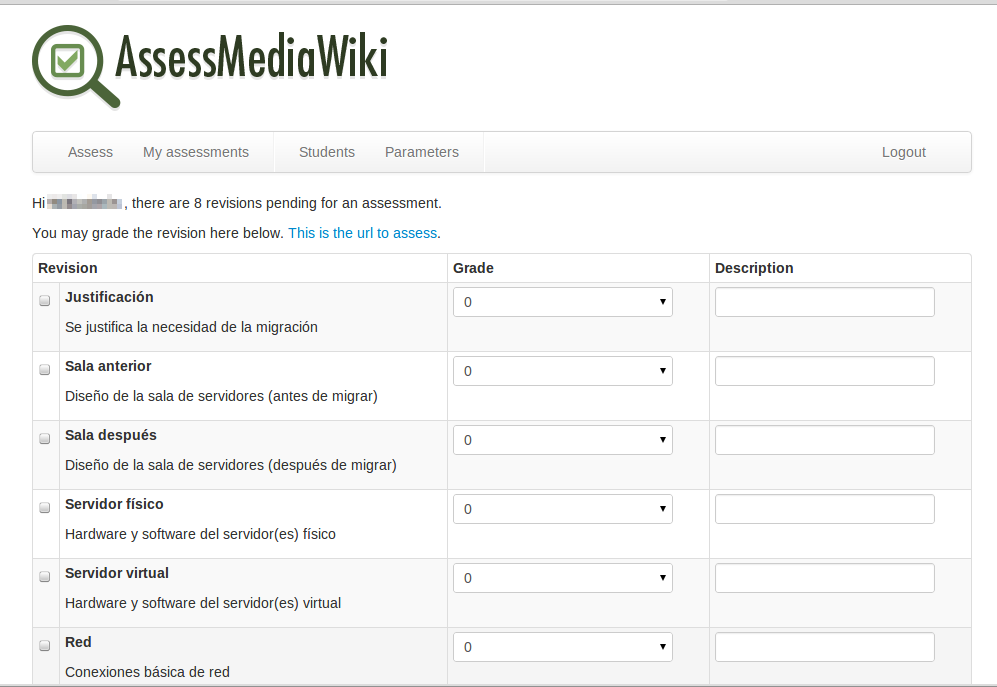
\includegraphics[scale=0.3]{AmwRubrica.png}
  \end{center}
  \caption{Rúbrica de AMW}
  \label{fig:AmwRubrica}
\end{figure}

		AMW implementa dos roles de usuario distintos: supervisores y estudiantes. Los estudiantes pueden elegir entre distintas opciones: evaluar una revisión, comprobar sus propias aportaciones evaluadas y verificar las evaluaciones ya enviadas. Por otro lado, los supervisores tienen un mayor número de opciones, como definir la rúbrica que los estudiantes deberán completar al realizar sus evaluaciones, modificar los parámetros de los programas o vigilar las evaluaciones que los alumnos vayan haciendo. AMW implementa una función de selección parcialmente aleatoria. Cuando un estudiante va a realizar una evaluación, el sistema elige automáticamente una de entre el 30\percentage más significativa que aún no ha sido evaluada.

		Al revisar sus evaluaciones, los estudiantes puede revisar las notas recibidas y sus justificaciones, así como ver a qué contribución en particular se refiere (figura~\ref{fig:AmwFormative}). Si el estudiante no está de acuerdo con la calificación puede replicar utilizando para ello una rúbrica similar a la que se utilizó en su evaluación, indicando las calificaciones que considera que merece y sus correspondientes justificaciones. Después el profesor revisará la disputa y pondrá la nota definitiva.

\begin{figure}
  \begin{center}
    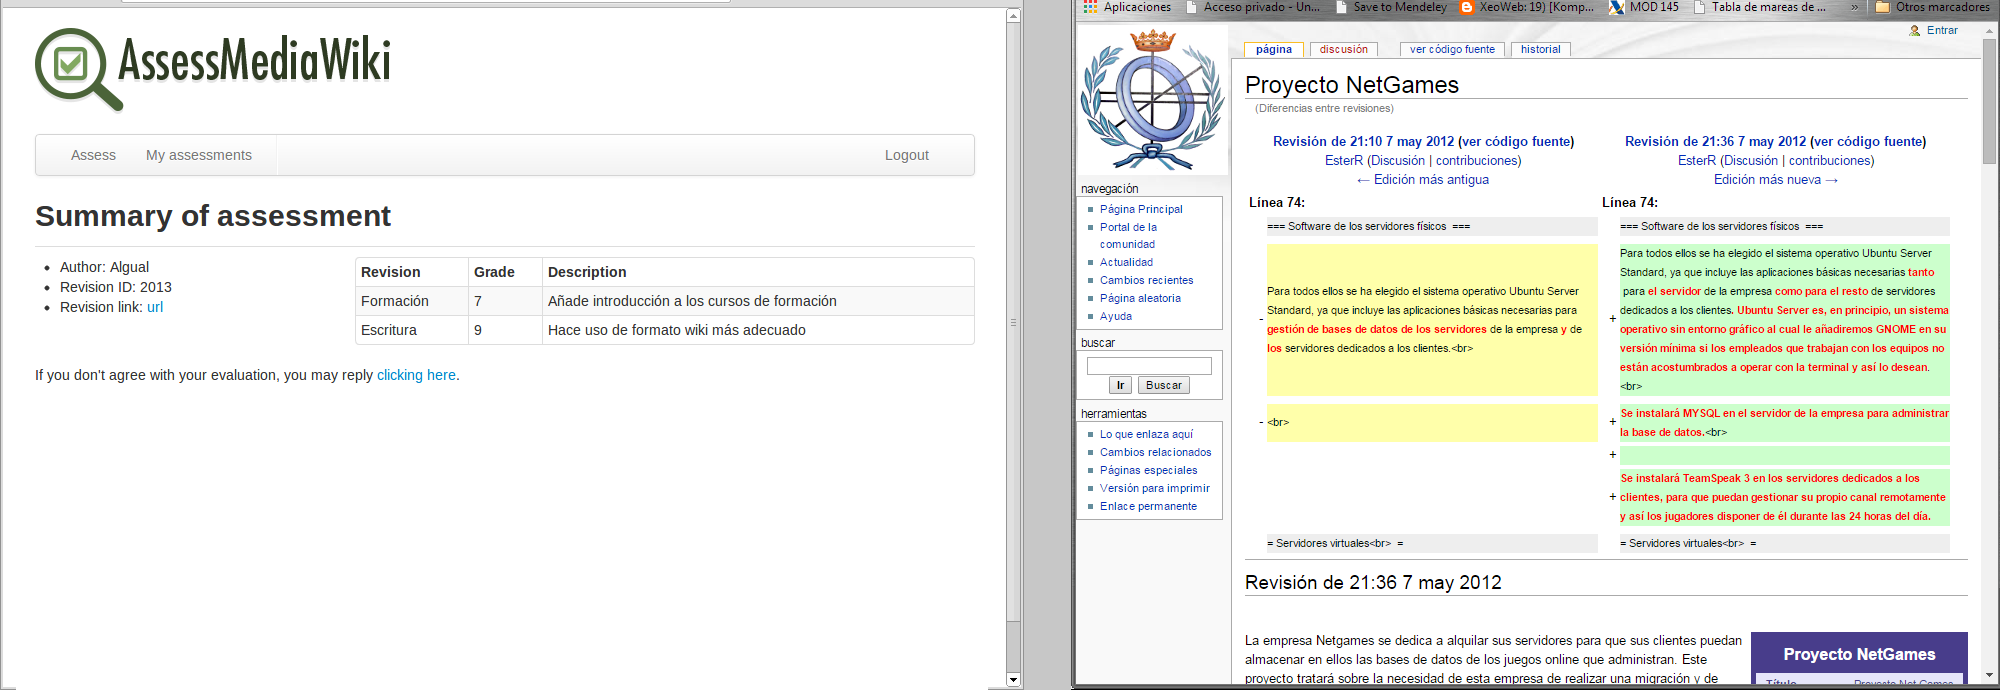
\includegraphics[scale=0.19]{AmwFormative.png}
  \end{center}
  \caption{Ejemplo de retroalimentación formativa y la contribución de wiki evaluada}
  \label{fig:AmwFormative}
\end{figure}

			\paragraph{Ejemplo de uso}

			El método para la evaluación del trabajo y las competencias desempeñadas en el wiki consta de dos partes: una primera parte en la que lo que se evalúa es el trabajo del wiki (A), basada en procedimientos de autoevaluación, evaluación entre iguales y evaluación del profesor; y una segunda parte en la que se evalúan las competencias genéricas (B) y en la que se pone en práctica el \emph{ciclo de contraste de hipótesis}.

			\paragraph*{A. Evaluación del trabajo en el wiki.}

			El método para la evaluación del trabajo en el wiki se divide también en tres fases: una primera fase en la que los estudiantes realizan sus trabajos en las páginas del wiki, una segunda fase de evaluación y una tercera fase de revisión del profesor. En la figura~\ref{fig:AmwDiagram} puede verse un diagrama de flujo de trabajo que muestra cada una de las fases del método de evaluación realizado sobre una página del wiki en la que participan varios estudiantes y el profesor. A continuación se describen cada una de estas fases.

\begin{figure}
  \begin{center}
    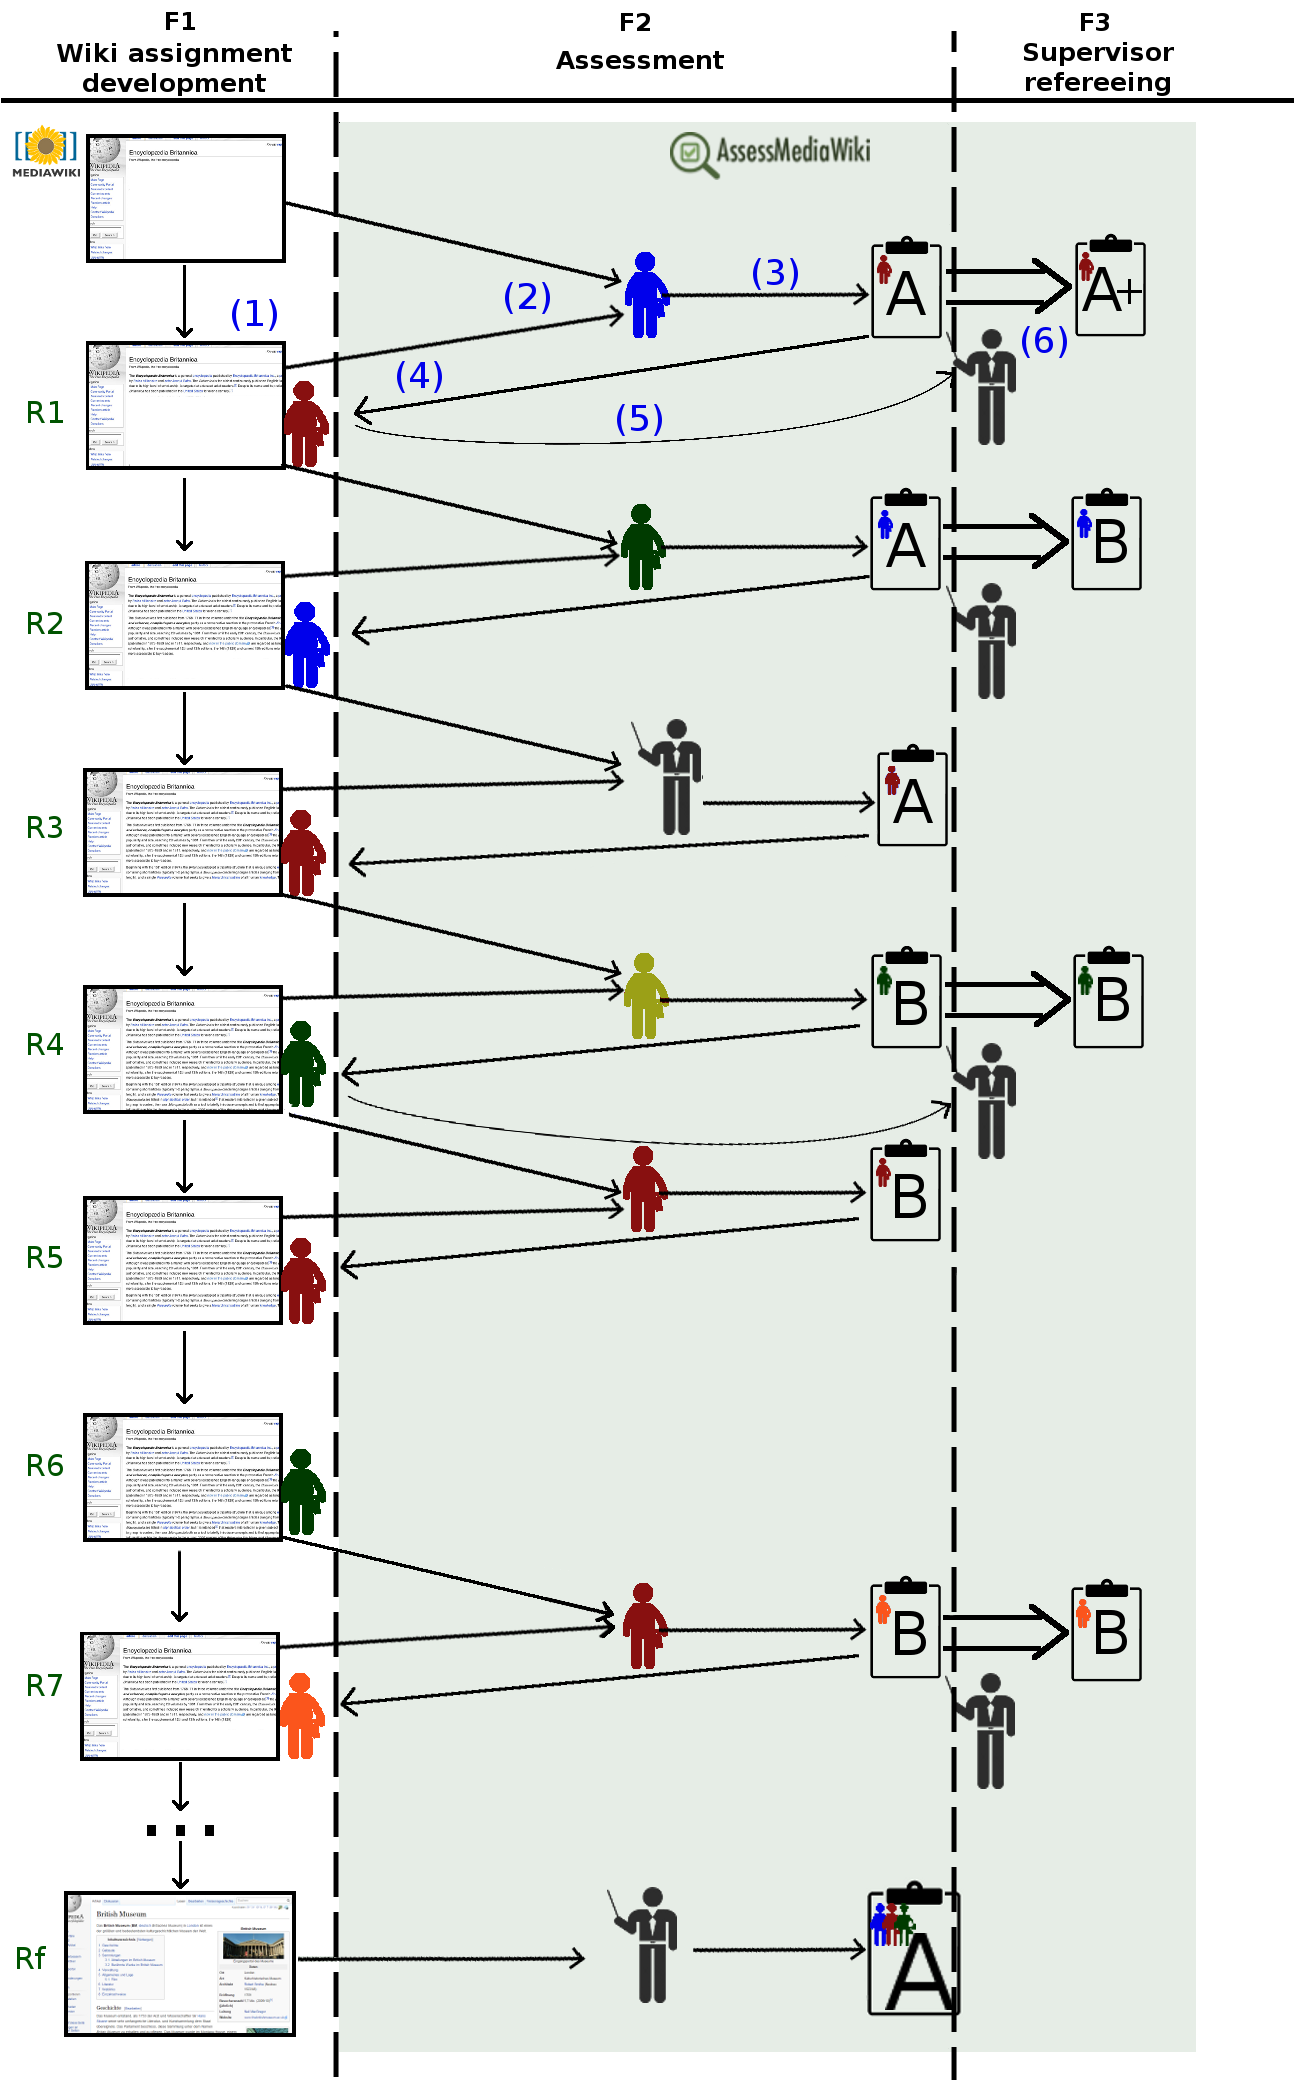
\includegraphics[scale=0.28]{AmwDiagram.png}
  \end{center}
  \caption{Ejemplo de flujo de trabajo para la evaluación cualitativa del wiki utilizando AMW}
  \label{fig:AmwDiagram}
\end{figure}

			\subparagraph*{Fase 1: Desarrollo del trabajo en el wiki.}

			Esta fase se representa en la columna de la izquierda de la figura~\ref{fig:AmwDiagram}, y es en la que los estudiantes realizan el trabajo en las páginas del wiki. Normalmente, cada grupo de estudiantes tendrá que desarrollar su trabajo en una página del wiki. En la zona más alta de la columna se representa el comienzo del trabajo con una página en blanco. El autor de cada contribución se muestra con una figura de color junto a la misma. Para comenzar, el usuario de color rojo crea una página vacía (\emph{R1}). Después, el usuario azul añade contenido a la página (\emph{R2}). En tercer lugar, el usuario rojo modifica de nuevo la página añadiendo texto a la versión dejada anteriormente por el usuario azul (\emph{R3}) y así sucesivamente. Esta fase termina cuando llega la fecha marcada por el profesor para que los trabajos estén finalizados (\emph{Rf} es la versión final de la página).

			Puede verse que, aunque los estudiantes responsables de la página de ejemplo del wiki fuesen el rojo, el azul y el verde, otros estudiantes, como el naranja en la revisión séptima, podrían contribuir a la página del wiki. En ese caso, los miembros del grupo y responsables de la página deben decidir si la contribución debe conservarse o no.

			\subparagraph*{Fase 2: Evaluación.}

			Esta fase se muestra en la columna central y comprende las siguientes actividades:

			\begin{itemize}
				\item \emph{Autoevaluación, evaluación entre iguales y evaluación del profesor}. Las contribuciones a ser evaluadas se asignan a los estudiantes.  Cada contribución es la diferencia entre dos revisiones consecutivas de una página del wiki. El estudiante encargado de evaluar dicha contribución se representa en el gráfico como un usuario coloreado que recibe dos flechas de las revisiones, una de la revisión anterior a la contribución y otra de la revisión que incorpora ya la contribución. Para la evaluación los estudiantes utilizan una rúbrica definida por el profesor. Cada contribución sólo se refiere a una contribución atómica de las realizadas a una página del wiki por un único estudiante, por lo que dicha contribución podría ser utilizada como un indicador de la contribución al wiki de dicho estudiante. El estudiante que realizó cada contribución se representa con una figura pegada a la revisión de la página en cada momento.
Por ejemplo, en la primera evaluación, se asigna la contribución realizada a la página del wiki por el estudiante rojo (\emph{1}) al estudiante azul. El estudiante azul comprueba ambas versiones para ver las diferencias entre ambas versiones (\emph{2}) y realiza la evaluación completando la rúbrica proporcionada por el profesor (\emph{3}).
Cabe destacar también otras situaciones interesante. En la versión \emph{R5} de la página vemos como se realiza una autoevaluación, ya que el estudiante rojo, autor de la versión, es el mismo que tiene que evaluar su contribución. Vemos también que en \emph{R3} es el profesor el que realiza la evaluación de la contribución del estudiante rojo. Esto puede deberse a que el estudiante manualmente detecta una contribución que considera oportuna evaluar o a que, utilizando la herramienta SMW, detecta un comportamiento extraño en el wiki y quiere contrastar la situación. 
Puede verse también que hay contribuciones que no reciben evaluación alguna, como ocurre con \emph{R6}. Está claro que sería deseable que todas las contribuciones significativas fueran evaluadas, pero no es escalable.
				\item \emph{Revisión de las evaluaciones recibidas}. Los estudiantes pueden revisar las evaluaciones recibidas. Ellos pueden no sólo ver las notas que han recibido con las justificaciones y comentarios que añadieron sus evaluadores, sino también el enlace a la contribución. De esta forma, los estudiantes evaluados reciben una retroalimentación formativa. En la primera de las evaluaciones del diagrama de ejemplo puede verse como el estudiante rojo puede ver su evaluación (\emph{4}).
				\item \emph{Réplica}. Si el estudiante evaluado no está de acuerdo con la evaluación recibida tiene la opción de replicarla justificando el motivo de dicha réplica. En el diagrama de ejemplo puede verse como el estudiante rojo considera injusta su evaluación y realiza una réplica (\emph{5}). El profesor deberá resolver la réplica en la siguiente etapa.
				\item \emph{Evaluación final del wiki}. El profesor evalúa la versión final de la página del wiki desarrollada por cada grupo de estudiantes. Esta evaluación es necesaria ya que el objetivo principal de la tarea es que los estudiantes realicen un buen trabajo en una página del wiki. Como cualquier otra tarea, deberá ser evaluada por el profesor conforme al programa de estudios. Además, algunos de los criterios de evaluación sólo pueden ser evaluados en la versión final de la página, como por ejemplo, la coherencia del texto. De esta forma, aquellas contribuciones del wiki descartadas por la función de selección serán ahora implícitamente evaluadas ya que están integradas en el entregable final. Puede verse la evaluación al final del diagrama de ejemplo (\emph{Rf}), y cómo afecta al grupo de estudiantes completo.
\end{itemize}

			El diagrama no recoge algunas situaciones que también podrían darse. Por ejemplo, alguna contribución podría ser evaluada por más de un usuario, ya fuera otro estudiante o el profesor. También, para simplificar, el diagrama sólo muestra una calificación para la contribución (A, A+, B, ... etc.), pero las evaluaciones son multidimensionales.

			Un componente interesante de nuestro algoritmo es qué contribución wiki podrá ser asignada a cada estudiante para su evaluación. Es lo que llamamos \emph{función de selección}, y tiene varios aspectos a tener en cuenta:

			\begin{itemize}
				\item \emph{¿Debería cierta contribución en el wiki ser evaluada por más de un estudiante?} En realidad, tener varias evaluaciones de estudiantes diferentes sobre una misma contribución podría ser interesante para perfeccionar su evaluación y podría proporcionar información al profesor para evaluar no sólo al estudiante autor de la contribución, sino también a los evaluadores. De hecho, el número de contribuciones a ser evaluadas es dependiente del objetivo del experimento y su configuración. Cuánto más grande sea el experimento, más contribuciones susceptibles de ser evaluadas tendrá. Sin embargo, el número de evaluaciones que un estudiante puede realizar es limitado (para que siga siendo formativo). Por lo que cada evaluación adicional a la misma contribución provocará que otras contribuciones sean más pobremente evaluadas o que no lo sean.
				\item \emph{¿Qué contribuciones deberían ser evaluadas?} La importancia de evaluar cada contribución puede variar. Por ejemplo, evaluar al menos una mínima cantidad de contribuciones por cada estudiante, página o categoría sería interesante. Pero algunas contribuciones que añadan ciertas características al trabajo pueden ser relevantes o informativas sobre el trabajo realizado por un estudiante. Por ejemplo, aunque las contribuciones que añadan gran cantidad de texto suelan ser más interesantes que las contribuciones pequeñas, una contribución pequeña puede ir relacionada con el cambio de sentido de alguna frase o párrafo. De cualquier forma, un estudiante puede solicitar que una contribución en particular sea evaluada, aunque ésta quede fuera de la función de selección.
				\item \emph{¿Quién evalúa cada contribución?} Depende de la importancia que se quiera dar a la autoevaluación, la evaluación del compañero y la del profesor. De nuevo, se debería balancear el esfuerzo requerido y el detalle a exigir en las evaluaciones.
			\end{itemize}


			\subparagraph*{Fase 3: Revisión del profesor.}

			En esta última columna se representan dos actividades que corresponden al profesor:

			\begin{itemize}
				\item Resolución de las réplicas: el profesor revisa las réplicas indicando si proceden o no. En caso de que procedan, modifica la calificación. En el diagrama se puede ver como en la primera contribución, el estudiante rojo realiza una réplica (\emph{5}) sobre la evaluación reciba por el usuario azul (\emph{3}). El profesor revisa la réplica, la considera apropiada y modifica la calificación (\emph{6}). En un segundo ejemplo, en la evaluación realizada por el estudiante de color amarillo sobre la contribución realizada por el usuario de color verde puede verse como el profesor no acepta la réplica realizada por este último, y mantiene la calificación otorgada inicialmente por el estudiante amarillo.
				\item Revisión de evaluaciones no replicadas: el profesor puede revisar aleatoriamente otras evaluaciones realizadas por los estudiantes que no hayan sido replicadas. En el diagrama puede verse como en el profesor revisa las evaluaciones realizadas sobre las contribuciones representadas en \emph{R2} y en \emph{R7}, disminuyendo la calificación de la primera y manteniendo la segunda.
			\end{itemize}

			\paragraph*{B. Evaluación de competencias genéricas}

			El método para la evaluación de competencias genéricas se basa en el \emph{ciclo de contraste de hipótesis}. En la figura~\ref{fig:AmwDiagram2} puede verse la descripción del ciclo. Esta evaluación se puede llevar a cabo durante o después de que los estudiantes hayan realizado su trabajo en el wiki y sus evaluaciones con AMW. Evidentemente, cuánto más avanzado esté el trabajo más datos habrá para analizar. 

			El ciclo comienza con el diseño de un indicador por parte del profesor que podría plasmar en una hoja de cálculo a partir de los datos que recibirá de las evaluaciones (a). A continuación, el profesor realiza la petición a AMW que le proporcionará los datos (b). AMW consulta y procesa los datos en las bases de datos de MediaWiki y AMW (c) y se los envía al profesor (d). El profesor los integra en la hoja de cálculo previamente diseñada y los analiza (e). Si son válidos para la evaluación finaliza el proceso (f). Por el contrario, si necesitan algún tipo de refinamiento el profesor puede rediseñar la evaluación (g) y hacer una nueva petición.

\begin{figure}
  \begin{center}
    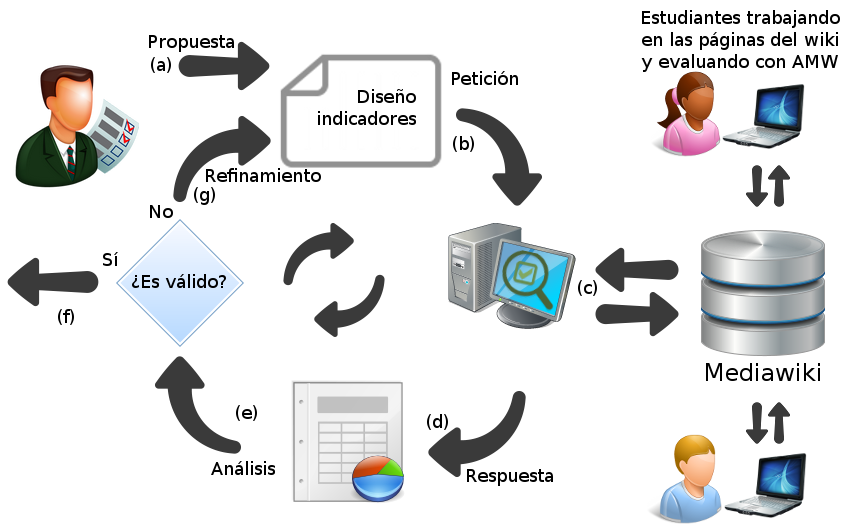
\includegraphics[scale=0.45]{AmwDiagram2.png}
  \end{center}
  \caption{Ciclo de contraste de hipótesis para la evaluación en wikis}
  \label{fig:AmwDiagram2}
\end{figure}

			\paragraph*{Indicadores de competencias genéricas}

				Los indicadores que se mencionan en este punto han sido utilizados en los estudios de caso realizados para este trabajo, pero como se ha mencionado desde un primer momento, este método proporciona indicadores y es el profesor el que los utilizará para evaluar las competencias genéricas que considere oportunas.

			\subparagraph*{Trabajo en equipo.}
			El indicador considerado para el trabajo en equipo es el \emph{ratio de miembros del equipo que trabajaron en un mismo criterio.} La rúbrica que utilizan los estudiantes para evaluar se compone de un conjunto de criterios. Cada criterio puede hacer referencia a una parte del trabajo. En todas las ediciones de un wiki no se trabajan en las mismas partes del trabajo, por lo que al ser evaluado, un estudiante puede tener nota en unos criterios y no tenerla en otros. Si más de un estudiante ha trabajado en la misma parte de una página wiki y su aportación ha sido significativa, tendrán nota en dicho criterio. Por tanto, partiendo de la cantidad de criterios que tiene un trabajo y del ratio de miembros del equipo que ha trabajado en cada criterio tendremos un indicador del trabajo en equipo.

			\subparagraph*{Comunicación y aplicación del conocimiento.}
			El indicador considerado para la comunicación y la aplicación del conocimiento es la \emph{media de las notas recibidas por todos los miembros del grupo}. Este indicador mide la incidencia que tuvieron las contribuciones realizadas en el éxito del proyecto. Una calificación pobre en una contribución puede significar  que alguna contribución wiki obtuvo una buena nota en un cierto criterio de la rúbrica pero una mala nota en el otro (el autor de la contribución soluciona un problema y crea uno nuevo). Probablemente, esto se debió a una mala comunicación entre los miembros del equipo o poco compromiso de un determinado alumno en el objetivo global del grupo. 

			\subparagraph*{Mantener la calidad del trabajo producido.}
			El indicador considerado para el mantenimiento de la calidad del trabajo producido es la \emph{media de las notas que cada estudiante individualmente recibió}. Unas calificaciones altas en las evaluaciones recibidas pueden significar que el trabajo que el estudiante está produciendo es de calidad. Si el estudiante produjese mucho contenido, pero este no fuese de calidad, las calificaciones no serían buenas. Es decir, sus calificaciones están teniendo en cuenta el aspecto cualitativo del trabajo y por tanto una nota alta significaría un trabajo de calidad.

			\subparagraph*{Capacidad crítica.}
			El indicador considerado para la capacidad crítica es el \emph{número de evaluaciones que el estudiante realizó con respecto al número de dichas evaluaciones cuya nota fue modificada por el profesor}. Este indicador mide la competencia de un estudiante para evaluar el trabajo hecho por otros. Si recibiera un número fijado de réplicas en sus revisiones y estas fueran revisadas por el profesor modificando las calificaciones, podríamos considerar que dicho alumno no ha desempeñado bien dicha competencia.

			En la tabla~\ref{tab:ResumenIndicadoresCualiCuanti} puede verse una comparación entre los indicadores considerados a partir de la evaluación cualitativa que se realizaría con AMW y los que se obtienen a partir de la evaluación cuantitativa realizada con SMW.

\begin{table}
  \begin{center}
  \begin{tabular}{| m{3.2cm} | m{4.9cm} | m{5.1cm} |}
    \hline 
    \multirow{2}{*}{COMPETENCIAS}  & INDICADORES  & INDICADORES  \\
      &  CUALITATIVOS  &  CUANTITATIVOS \\
    \hline
    \hline
    Trabajo en equipo  & Ratio de miembros del equipo que trabajaron en un mismo criterio  & Ratio de miembros del equipo que contribuyeron a una misma página del wiki en las páginas de su proyecto \\
    \hline
    Comunicación y aplicación del conocimiento  & Media de las notas recibidas por todos los miembros del grupo  & Porcentaje de miembros del equipo que contribuyeron al menos a un 20\percentage del trabajo realizado \\
    \hline
    Mantener la calidad del trabajo producido  & Media de las notas que cada estudiante individualmente recibió  & Contribución individual en bytes \\
    \hline
    Capacidad crítica  & Número de evaluaciones que el estudiante realizó con respecto al número de dichas evaluaciones cuya nota fue modificada por el profesor  & No considerada \\
    \hline
  \end{tabular}
\end{center}
\caption{Resumen de las competencias evaluadas para cada tipo de indicador}
\label{tab:ResumenIndicadoresCualiCuanti}
\end{table}

			\paragraph{Conclusiones}

			AMW es una herramienta de evaluación asistida que proporciona un análisis cualitativo interesante, pues al análisis cuantitativo proporcionado por StatMediWiki, se podría añadir una información cualitativa que impidiera el engaño de los estudiantes. Por ejemplo, la contribución de un estudiante que copiase y pegase una gran cantidad de texto en una página del wiki sería considerada a efectos cuantitavos como una contribución de peso. Sin embargo, desde un punto de vista cualitativo, podría detectarse que la contibución había sido plagiada de internet con el fin de engañar al sistema.

			Sin embargo, en la aplicación de AMW nos encontramos con que se dan algunos de los problemas detectados en la revisión de la literatura para este tipo de herramientasde evaluación asistida. En primer lugar, delegar la evaluación en los estudiantes genera situaciones de subjetividad, pues pueden existir apartados en la rúbrica que los estudiantes interpreten o valoren de forma diferente. Y en segundo lugar, como vemos en el diagrama, el profesorado también revisa las evaluaciones de sus estudiantes, y más aun si estos replican, con lo que los problemas de escalabilidad también aparecerían.

	\subsection{Implementación mediante DSL}

		Un DSL es un pequeño lenguaje de programación de gran potencia expresiva que se enfoca a un dominio particular. Los beneficios de utilizar un DSL son~\cite{vanDeursen:2000}:
		\begin{itemize}
			\item La solución a los problemas pueden ser expresados en un idioma y al nivel de abstracción del dominio del problema, y como consecuencia, los expertos en el dominio pueden entenderlo, validarlo, modificarlo y desarrollar sus propias soluciones.
			\item Los programas son concisos, autodocumentados en gran medida y reutilizables para diferentes propósitos.
			\item Mejora la productividad, la fiabilidad, la mantenibilidad y la portabilidad.
			\item Permite la validación y optimización al nivel del dominio.
			\item Mejora la capacidad de ser probado.
		\end{itemize} 

		A continuación se presentan los dos DSL que se han desarrollado para la implementación del método, cada uno aplicable a un contexto diferente. En el apartado~\ref{subcha:evc} se presenta el primer DSL, orientado para obtener indicadores de los VLEs, mientras que en el apartado~\ref{subcha:evs} se presenta el segundo DSL, orientado a los mundos virtuales. 

		\subsubsection{EvalCourse (EVC) y SASQL} \label{subcha:evc}

 %, los investigadores de diferentes áreas han colaborado para extraerlos, realizar minería de datos y utilizarlos para mejorar el aprendizaje~\cite{park2015development}.

		%Además, los autores de algunos de los trabajo recopilados en el estado del arte (capítulo~\ref{cha:State of the Art}) confirman la relación entre la interacción que llevan a cabo los estudiantes en el VLE y su rendimiento en el desempeño de varias competencias genéricas~\cite{fidalgo:2015,rayon2014web}.

% ¿Quitar la cita de vanDeursen? Está antes?
	El VLE es el núcleo de los cursos virtuales, donde los estudiantes acceden para interactuar con el curso. La interacción de los estudiantes genera gran cantidad de información que queda registrada en el VLE. Esta interacción será la base para los indicadores del desempeño de competencias genéricas.

			\paragraph{Descripción} % Análisis y diseño

			Para diseñar evaluaciones a partir de los indicadores del VLE se crea \emph{Simple Assessment-Specific Query Language} (SASQL). SASQL es un lenguaje formal para la ejecución automática de consultas simples escritas utilizando un lenguaje específico de evaluación. SASQL tiene un sintaxis simple, con términos del dominio docente y orientado a la evaluación de competencias genéricas~\cite{Balderas:2013}. De esta forma, los profesores pueden fácilmente obtener indicadores almacenados de la actividad en el VLE sin requerir conocimientos técnicos en bases de datos o programación informática.

			También se implementa \emph{EvalCourse}, una herramienta informática que ejecuta instrucciones escritas en SASQL, proporcionando como resultado los indicadores solicitados. EvalCourse se comunica con el VLE para extraer la información del registro de actividad. EvalCourse\footnote{https://www.assembla.com/spaces/evalcourse} está basado en el IDE de la plataforma Eclipse, fue implementado utilizando Xtext~\cite{eysholdt2010xtext} dentro del Eclipse Modeling Framework y está disponible como software libre bajo licencia GNU GPL.

			El desarrollo de EvalCourse y SASQL se basa en los principios y técnicas de la ingeniería dirigida por modelos (MDE, del inglés Model-Driven Engineering). Este enfoque promueve la construcción de artefactos software de un modo flexible y rápido mediante el desarrollo de modelos y sus transformaciones. Nuestro DSL se define en términos de su sintaxis abstracta o metamodelo, su sintaxis concreta y un conjunto de plantillas para la transformación de modelos de consulta en código ejecutable dependiente del VLE.

\begin{figure}
  \begin{center}
    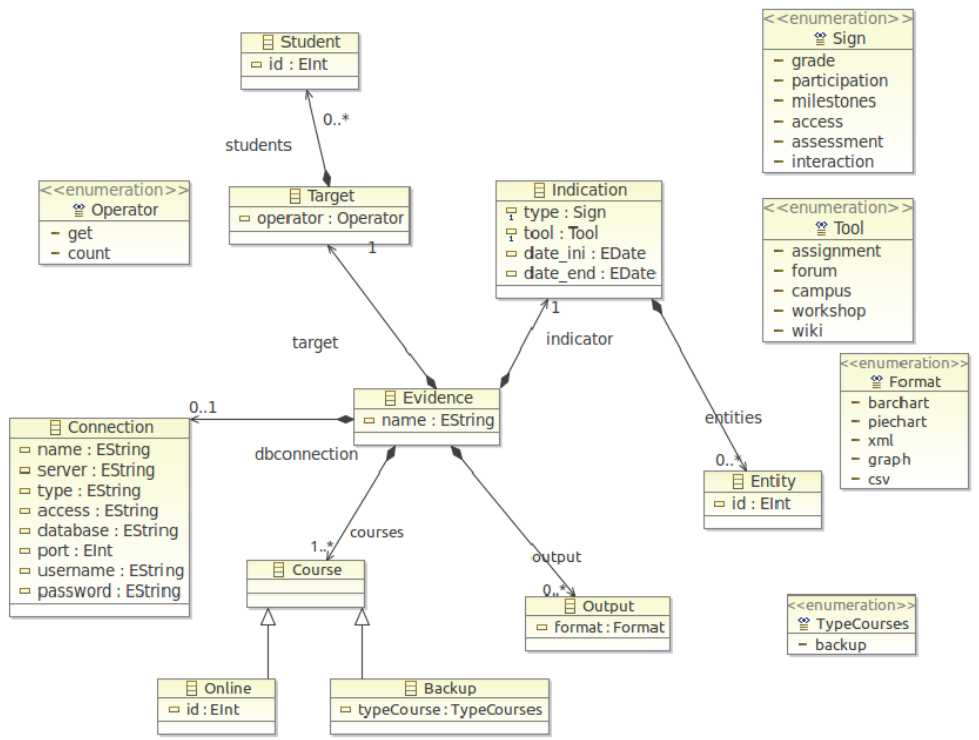
\includegraphics[scale=0.4]{EvcMetamodel.png}
  \end{center}
  \caption{Metamodelo de SASQL}
  \label{fig:EvcMetamodel}
\end{figure}

			El metamodelo de SASQL puede verse en la figura~\ref{fig:EvcMetamodel}. La entidad principal es el indicador o evidencia (\emph{evidence}). Esta evidencia se aplicará a una herramienta (\emph{tool}) que puede ser tarea (\emph{assignment}), foro (\emph{forum}), campus (\emph{campus}), taller (\emph{workshop}) o wiki (\emph{wiki}), en las que se observará un indicio (\emph{sign}), que puede ser participación (\emph{participation}), entregas (\emph{milestones}), accesos (\emph{access}), evaluaciones (\emph{assessment}), interacción (\emph{interaction}) o calificación (\emph{grade}). Además, puede actuarse sobre una actividad específica (\emph{entity}) o sobre todas las actividades de un tipo que se han dado en el VLE. La conexión a la base de datos del curso se declara en la entidad \emph{connection}. 

			La sintaxis de SASQL puede verse en la consulta~\ref{code:sasqlSintax}. En la primera línea se comienza con la palabra reservada \emph{Evidence} seguida del nombre que se dará al indicador. Ese nombre será el que tengan todos los ficheros de salida. En la segunda línea se escriben los términos obligatorios \emph{get students}. En la tercera, se indica qué indicio se quiere extraer (\emph{show milestones | participation | access | interaction | assessment | grade}). En la consulta, la tercera línea se divide en dos (tercera y cuarta) para que puedan ser visualizadas todas las opciones. En la quinta, se indica sobre qué herramienta se quiere obtener el indicio (\emph{ in assignment | forum | campus | workshop | wiki [list of ids]}). También la quinta línea se divide en dos (quinta y sexta). En la séptima línea, que es opcional, se indica el rango de fechas sobre los que se extraerá la información. Y por último, en la octava se especifica si la conexión se realizará directamente a la base de datos o sobre una copia de seguridad almacenada en un fichero.

\begin{lstlisting}[caption=Sintaxis de SASQL (las palabras reservadas se muestran resaltadas),label=code:sasqlSintax,numbers=left, captionpos=b, morekeywords={Evidence,get, students, show, milestones, participation, access, in, assignment, forum, campus, wiki, between, and, workshop, interaction, assessment, grade, from, course, backup}]
Evidence indicator_name:
 get students 
 show milestones | participation | access 
	| interaction | assessment | grade
 in assignment | forum | campus | workshop 
	| wiki [list of ids]
 between YYYY-MM-DD and YYYY-MM-DD
 from course id | backup.
\end{lstlisting}

			El objetivo es que EvalCourse pueda ser utilizado para cualquier VLE, pero esta primera versión ha sido implementada para funcionar en Moodle~\footnote{https://moodle.org/}. Moodle es un sistema de gestión de aprendizaje de código abierto con más de 64.000 sitios registrados~\footnote{https://moodle.net/stats}, y que además es el que se utiliza en la Universidad de Cádiz.


			\paragraph{Ejemplo}

			Para evaluar las competencias genéricas el profesor deberá definir los indicadores que serán extraídos de la actividad de cada estudiante en el VLE. Ilustraremos el método a partir de un ejemplo de uso de EvalCourse y su ejecución con los foros del VLE. Los foros suelen ser una de las herramientas incorporadas por los VLEs para la interacción entre los estudiantes. Es evidente que la comunicación oral es una manera muy rica de comunicarse, que proporciona múltiples signos no verbales como las expresiones faciales o el tono de voz. En contraste, las comunicaciones escritas proporcionan otras ventajas. Una de las más importantes para la educación es que el estudiante dispone de un tiempo para la reflexión. Por esta razón, podría preferirse la comunicación escrita a la oral cuando se busca un aprendizaje cognitivo~\cite{garrison1999critical}.

			La obtención de indicadores se basará en el \emph{ciclo de contraste de hipótesis}(figura~\ref{fig:EVCDiagram}). En primer lugar, es necesario que los estudiantes hayan interactuado en el VLE, de manera que su actividad haya quedado registrada. Entonces, el profesor propone un diseño de evaluación mediante una consulta SASQL (a) y envía esta consulta a EvalCourse (b). EvalCourse procesa la consulta, realiza la petición a la base de datos y recoge los datos (c). Entonces EvalCourse devuelve los resultados (d). El profesor analiza los resultados conforme a su propuesta de evaluación de competencias (e), terminando el proceso si éstos son válidos para él (f). Por el contrario, si los resultados no son válidos como indicadores de la competencia, entonces el profesor podrá rediseñar la evaluación (g). En cualquier caso, el profesor podrá reutilizar el diseño cuántas veces sea necesaria a lo largo del curso y monitorizar la evolución de los indicadores de cada estudiante.

\begin{figure}
  \begin{center}
    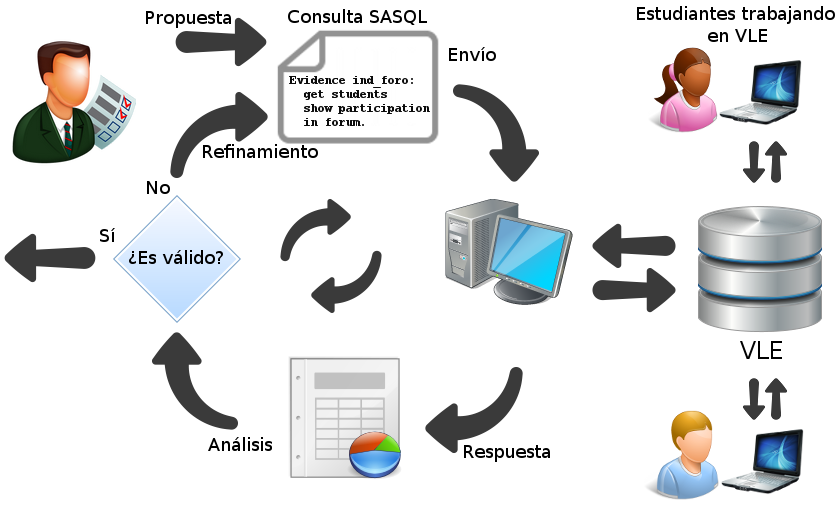
\includegraphics[scale=0.45]{EvcDiagram.png}
  \end{center}
  \caption{Ciclo de contraste de hipótesis utilizando EvalCourse}
  \label{fig:EVCDiagram}
\end{figure}

			En este ejemplo, el profesor pretende obtener indicadores del uso del foro para evaluar la competencia genérica de las habilidades interpersonales. Durante el curso, los estudiantes interactuarán en el foro conforme a las instrucciones proporcionadas por el profesor. Cuando lo desee, el profesor podrá utilizar EvalCourse para obtener los indicadores.

% Estos indicadores deben ser publicados para que los estudiantes sepan cómo serán evaluados % FRASE ELIMINADA DEL MEDIO DEL PÁRRAFO ANTERIOR

			El profesor considera que podría diseñar un indicador válido a partir del número de mensajes que ha escrito cada estudiante en un periodo de tiempo particular y plantea la siguiente hipótesis: \emph{se considerará que un estudiante ha desempeñado satisfactoriamente la competencia genérica de las habilidades interpersonales si ha escrito al menos dos mensajes en el foro}. Para ello se diseña la consulta~\ref{code:sasqlejemplo1}. EvalCourse procesa la consulta y devuelve los resultados que se pueden ver en la tabla~\ref{tab:EvalCourseEj1}.

\begin{lstlisting}[caption=Participación en el foro en un periodo concreto de tiempo ,label=code:sasqlejemplo1,numbers=left, captionpos=b, morekeywords={Evidence,get, students, show, milestones, participation, access, in, assignment, forum, campus, workshop, interaction, between, and}]
Evidence participacion_foro: 
	get students
	show participation
	in forum between 2015-10-21 and 2015-10-27.
\end{lstlisting}

\begin{table}
	\centering
	\caption{Información sobre la participación en el foro de los estudiantes en un periodo concreto de tiempo}
	\label{tab:EvalCourseEj1}
	\begin{tabular}{|l|l|c|c|c|c|c|}
		\hline
		id & username & Debate-starter & Debate-participation & Total \\
		\hline
		\hline
		1 & student1 & 1 & 2 & 3  \\
		\hline
		2 & student2 & 0 & 4 & 4  \\
		\hline
		3 & student3 & 0 & 1 & 1  \\
		\hline
		4 & student4 & 1 & 2 & 3  \\
		\hline
		5 & student5 & 0 & 2 & 2  \\
		\hline
	\end{tabular}
\end{table}

			A la vista de los resultados, y en base a la hipótesis inicial, se podría decir que todos los estudiantes menos el 3 (\emph{student3}) habrían desempeñado correctamente la competencia. Sin embargo, el profesor considera que esta primera aproximación es un poco pobre y decide completar su hipótesis de la siguiente manera: \emph{se considerará que un estudiante ha desempeñado satisfactoriamente la competencia genérica de las habilidades interpersonales si ha escrito al menos dos mensajes en el foro y ha interactuado con más de un compañero}. Para ello escribe la consulta~\ref{code:sasqlejemplo2}. 

\begin{lstlisting}[caption=Interacción en el foro en un periodo de tiempo ,label=code:sasqlejemplo2,numbers=left, captionpos=b, morekeywords={Evidence,get, students, show, milestones, participation, access, in, assignment, forum, campus, workshop, interaction, between, and}]
Evidence interacciones_foro: 
	get students
	show interaction
	in forum between 2013-10-21 and 2013-10-27.
\end{lstlisting}

			Además del listado con las interacciones, EvalCourse proporciona varias figuras con la representación de la información. Para esta última consulta se devuelve un grafo para una mejor visualización de las interacciones (figura~\ref{fig:EvalCourseInteraccionForo}). A tenor de los resultados vemos que sólo dos de los estudiantes cumplen la segunda hipótesis (\emph{student2} y \emph{student4}). 

\begin{figure}
	\centering
	\includegraphics[width=6cm]{{EvalCourseInteraccionForo.png}}
	\caption{Interacción en el foro en un periodo de tiempo.}
	\label{fig:EvalCourseInteraccionForo}
\end{figure}

			De esta manera, el profesor irá redefiniendo sus hipótesis hasta dar con los indicadores que a su juicio satisfagan la evaluación de la competencia genérica.

			\paragraph*{Propuesta de indicadores para el ejemplo}

			En este apartado se muestra una propuesta de uso de indicadores obtenidos mediante EvalCourse para la evaluación de competencias genéricas~\cite{Balderas:2015}. Pero al igual que ocurre con el resto de herramientas, estos indicadores podrían ser válidos para unos profesores y no serlos para otros, así como que habrá otras muchas formas de combinar la información del registro para obtener indicadores válidos para otras competencias genéricas.

				\paragraph*{Habilidades interpersonales}
				Para la evaluación de esta competencia genérica se propone utilizar la participación en el foro. Al crear grupos de trabajo en el VLE se puede crear un foro para cada grupo. Durante el curso se fomenta que los estudiantes intervengan en dichos foros para comunicarse entre los miembros del equipo y dejar constancia de los mensajes de cara al profesor. Por tanto, si no utilizan el foro, los estudiantes no tienen calificación en esta competencia. Por ejemplo, podría fijarse que un estudiante que tuviera tres o más intervenciones en el foro tendría una evaluación positiva en la competencia.

				\paragraph*{Liderazgo}
				Para evaluar el liderazgo de los estudiantes se proponen también los foros creados para la comunicación de los equipos de trabajo. Para ello se podría considerar la cantidad de debates que cada estudiante ha iniciado. Por ejemplo, un estudiante que iniciara dos o más debates tendría una evaluación positiva en la competencia de liderazgo.

				\paragraph*{Pensamiento crítico}
				En Moodle hay una actividad que son los talleres (\emph{workshops}). En esta actividad, los estudiantes tienen que entregar un ejercicio conforme a las instrucciones del profesor que podrá ser autoevaluada o evaluada por uno o varios compañeros. Por ejemplo, podría plantearse que cada estudiante tuviera que hacer varias tareas. Una vez entregada cada tarea, el profesor pondría la solución del ejercicio a disposición de los estudiantes, y cada tarea sería evaluada por dos compañeros y por el propio estudiante. Para evaluar la competencia del pensamiento crítico, el profesor utilizaría para cada tarea la diferencia entre la media de las notas dadas por sus compañeros y la que se asignó el propio estudiante.

				\paragraph*{Planificación y gestión del tiempo}
				Las tareas programadas en el VLE tienen una fecha límite de entrega. Sin embargo, el profesor puede configurar la actividad para que permita envíos retrasados. El profesor podría establecer un número mínimo de trabajos entregados antes de la fecha límite para considerar que esta se ha entregado a tiempo. De esta manera, un profesor podría considerar que si las tareas se han entregado tarde, pero son correctas, tengan una buena calificación en lo que a las habilidades y conocimientos específicos que requería la tarea se refiere. Pero con respecto a la planificación y gestión del tiempo de ese estudiante la calificación sería negativa, dado que ha incumplido la planificación y los plazos que se acordaron a comienzos del curso.

		\subsubsection{EvalSim (EVS) y VWQL} \label{subcha:evs}

		La segunda propuesta de DSL se aplica a los mundos virtuales. Aunque muchos investigadores han reconocido la potencia educativa y motivacional de los videojuegos, hay pocos estudios empíricos que hayan investigado recientemente su impacto en el aprendizaje de los estudiantes~\cite{berns2013game}. Lo mismo se puede decir de los entornos de aprendizaje como los mundos virtuales (Second Life, OpenCobalt, etc.)~\cite{hew2010use}. Esto se debe a que normalmente no se distribuyen bajo licencia libre y, por consiguiente, los profesores no pueden analizar las interacciones de los estudiantes o analizar su impacto en el aprendizaje y en los resultados de aprendizaje~\cite{cruz2015discovering,moreno2014serious}. 

		Ante esta situación, en un trabajo previo desarrollamos nuestro propio mundo virtual, basado en OpenSim (software de código abierto)~\cite{berns2013using}. De esta forma se podría evaluar la competencia de la comunicación en una segunda lengua a partir de las interacciones llevadas a cabo por los estudiantes en el mundo virtual.

		A continuación se explicará cómo a partir de la actividad generada por los estudiantes se obtendrán indicadores para el diseño de evaluaciones de competencias genéricas.

			\paragraph{Descripción}

			Para este trabajo se creó VWQL (\emph{Virtual Worl Query language}). VWQL es un DSL creado para obtener indicadores objetivos de OpenSim. EvalSim es el sistema que procesa las consultas de VWQL. Ha sido desarrollado bajo un enfoque MDE para modelar procesos para la obtención de los indicadores que se requieran. Fue también implementado utilizando Xtext~\cite{eysholdt2010xtext} dentro del Eclipse Modeling Framework.

			La sintaxis del lenguaje (versión beta 0.1) puede verse en la consulta~\ref{code:reserved}. La primera línea especifica el nombre del indicador (\emph{name\_of\_the\_indicator}) y se utiliza para diferenciar los diferentes archivos producidos por EvalSim. La segunda línea comienza obligatoriamente con \emph{get students} y a continuación se ha de especificar si se quiere obtener la información para todos los estudiantes que participaron en la experiencia o sólo para algunos de los que participaron (indicando sus identificadores numéricos de usuario). La última línea indica el tipo de información a extraer tras el término obligatorio \emph{show}, y esta información puede ser de alguno de los siguientes tipos:

\begin{itemize}
\item \emph{words}: número de palabras escritas en el chat de texto. Por defecto cuenta todas las palabras, a no ser que se indique un idioma, en cuyo caso únicamente muestra, de las palabras introducidas en el chat de texto, las palabras en dicho idioma.
\item \emph{sentences}: número de frases escritas en el chat de texto.
\item \emph{single}: número de frases compuestas por una sola palabra escritas en el chat de texto.
\item \emph{turns}: número de turnos empleados en chat de texto. Un turno es un conjunto de frases consecutivas escritas por el mismo usuario.
\item \emph{time}: número de minutos jugados en el mundo virtual.
\item \emph{points}: número de puntos obtenidos en el mundo virtual. La manera en que los puntos se obtengan dependerá específicamente del mundo virtual jugado.
\end{itemize}

\begin{lstlisting}[caption=Palabras reservadas y formato de VWQL (version 0.1), label=code:reserved,numbers=left, captionpos=b, morekeywords={Evidence,get, students, show, words, sentences, turns, time, points}]
Evidence name_of_the_evidence:
    get students [id_of_the_student]
    show ( words [dict] | sentences | turns |
         | time | points )+
\end{lstlisting}

			\paragraph{Ejemplo}

			En el juego los estudiantes interactúan entre ellos por medio de un chat. Las conversaciones quedan almacenadas en la base de datos de EvalSim. Utilizando el \emph{ciclo de contraste de hipótesis} los profesores obtendrán indicadores del trabajo de sus estudiantes (figura~\ref{fig:EvsDiagram}).

\begin{figure}
  \begin{center}
    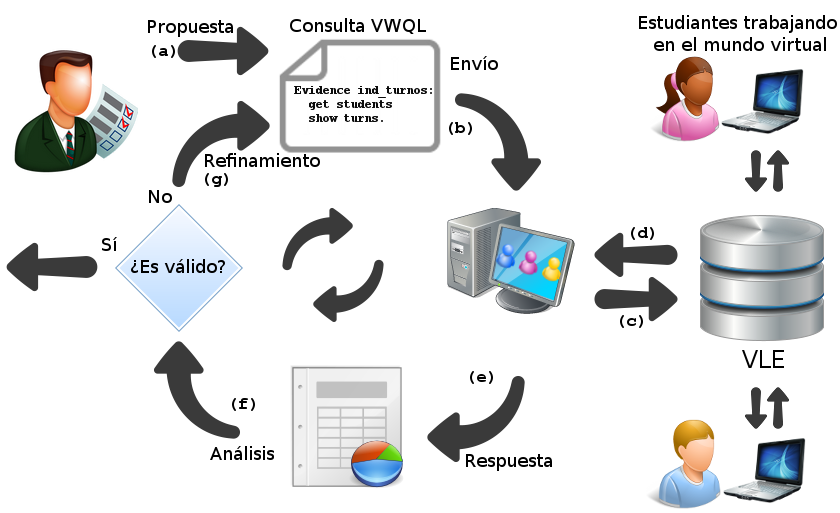
\includegraphics[scale=0.4]{EvsDiagram.png}
  \end{center}
  \caption{Ciclo de contraste de hipótesis con EvalSim}
  \label{fig:EvsDiagram}
\end{figure}

			El profesor propone una evaluación (\emph{a}) que bajo su criterio le vaya a proporcionar indicadores válidos para evaluar alguna competencia genérica y la envía a EvalSim (\emph{b}). EvalSim procesa la petición y realiza la solicitud a la base de datos del mundo virtual (\emph{c}) . Una vez que recibe los datos (\emph{d}), los transforma y devuelve los resultados debidamente formateados al profesor (\emph{e}). El profesor los analiza, y si considera que son indicadores válidos para evaluar la competencia (\emph{f}) termina el ciclo. Sin embargo, si entiende que no les sirven o considera que debería refinarlo podría volver a diseñar una nueva evaluación (\emph{g}), reiniciándose de nuevo el ciclo.


			%\paragraph{Ejemplo de uso}

			En este ejemplo se parte de que el mundo virtual se está utilizando en una asignatura de idiomas. En un ejercicio práctico confeccionado por el profesor, los estudiantes han de participar en un juego de roles (\emph{role-play}) y son advertidos de que deben explayarse en sus respuestas a fin de utilizar los recursos lingüísticos aprendidos en clase.

			Una vez que todos los estudiantes han participado el juego, el profesor decide utilizar como indicador el número de frases de una sola palabra utilizada por los estudiantes. De esta manera, todos aquellos estudiantes que hayan utilizado una sola palabra para responder a alguna pregunta tendrán una evaluación negativa en el desempeño de la competencia. Puede verse el código empleado en la consulta~\ref{code:vqwlej1}.

\begin{lstlisting}[caption=Respuestas de una sola palabra, label=code:vqwlej1,numbers=left, captionpos=b, morekeywords={Evidence,get, students, single, show, words, sentences, turns, time, points}]
Evidence respuestas_cortas:
    get students
    show single.
\end{lstlisting}

			Como resultado a la consulta, el sistema devuelve el listado que puede verse en la tabla~\ref{tab:EvsListEj1}. A la vista de los mismos, el profesor considera que hay situaciones en las que una respuesta corta podría admitirse como válida, por lo que decide admitir como mucho dos respuestas cortas en la participación de cada estudiante. Ante este enfoque, el profesor considera que los estudiantes 3, 6 y 7 (\emph{studen3, student6 y student7}) tuvieron un desempeño bajo en la competencia al haber empleado cuatro, cuatro y tres respuestas cortas respectivamente.

\begin{table}
	\centering
	\caption{Información sobre las respuestas de una sola palabra dadas por los estudiantes en el role-play}
	\label{tab:EvsListEj1}
	\begin{tabular}{|l|l|c|}
		\hline
		id & username & singles \\
		\hline
		\hline
		1 & student1 & 0  \\
		\hline
		2 & student2 & 1  \\
		\hline
		3 & student3 & 4  \\
		\hline
		4 & student4 & 0  \\
		\hline
		5 & student5 & 2  \\
		\hline
		6 & student6 & 4  \\
		\hline
		7 & student7 & 3  \\
		\hline
		8 & student8 & 1  \\
		\hline
	\end{tabular}
\end{table}

			Para enriquecer este indicador, el profesor decide diseñar un nuevo indicador. En este caso, calculando el número de palabras por turno que escriben los estudiantes. Para ello utiliza la consulta~\ref{code:vqwlej2}. Los resultados en este caso puede verse en la tabla~\ref{tab:EvsListEj2}.

\begin{lstlisting}[caption=Respuestas de una sola palabra, label=code:vqwlej2,numbers=left, captionpos=b, morekeywords={Evidence,get, students, single, show, words, sentences, turns, time, points}]
Evidence palabras_turno:
    get students
    show words, turns.
\end{lstlisting}

\begin{table}
	\centering
	\caption{Información sobre las palabras por turnos utilizadas por los estudiantes en el role-play}
	\label{tab:EvsListEj2}
	\begin{tabular}{|l|l|c|c|c|}
		\hline
		id & username & words & turns & words per turn \\
		\hline
		\hline
		1 & student1 & 117 & 9 & 13 \\
		\hline
		2 & student2 & 132 & 11 & 12  \\
		\hline
		3 & student3 & 63 & 9 & 7  \\
		\hline
		4 & student4 & 140 & 10 & 14  \\
		\hline
		5 & student5 & 99  & 11 & 9 \\
		\hline
		6 & student6 & 80 & 10 & 8  \\
		\hline
		7 & student7 & 72 & 9 & 8  \\
		\hline
		8 & student8 & 108 & 9 & 12   \\
		\hline
	\end{tabular}
\end{table}

			A la vista de los resultados, el profesor confirma que los estudiantes 3, 6 y 7 (\emph{studen3, student6 y student7}) son los que utilizan menos palabras por turno. Son estos tres estudiantes, junto con el estudiante número 5 (\emph{student5}), los únicos que bajan de 10 palabras por turno. Lo que podría ser una justificación para el profesor a la hora de evaluar de manera negativa a este estudiante, ya que no sólo no llega a 10 mensajes sino que también es el único que en la consulta anterior está en el límite fijado de dos respuestas cortas.

			Como en los casos anteriores, será decisión del profesor el uso que se dé a los indicadores.

			\paragraph*{Propuesta de indicadores para el ejemplo}

			El mundo virtual se ha desarrollado para asignaturas de idiomas, por lo que la competencia genérica para la que más se han utilizado los indicadores obtenidos ha sido para la \emph{habilidad para comunicarse en un segundo idioma}. Aunque sólo es una propuesta y podrían utilizarse también para otras competencias.

% Hipótesis: un estudiante tiene dificultades para hacerse entender si necesita dos o más frases por turno para comunicarse con su compañero.

			\subparagraph*{Segundo idioma}
\begin{itemize}
\item \emph{Ritmo}: número de frases escritas por minuto. Según la experiencia desarrollada podría ser un indicador positivo o negativo del desempeño de la competencia. Si el estudiante tiene que contar una historia o expresarse sin restricción, el hecho de que escriba muchas frases por minuto es un indicador positivo de su dominio del idioma. Sin embargo, si el estudiante tiene que enviar a su compañero un mensaje concreto y tiene dificultades  para hacerse entender, puede necesitar más de una frase por minuto para hacerse entender, siendo entonces un indicador negativo.
\item \emph{Frases por turno}: número de frases escritas por turno. Igual que en el caso anterior, puede tomarse como un indicador positivo o negativo dependiendo del caso. Si el estudiante tiene un buen dominio del idioma y no hay restricción impuesta, puede ser un indicador positivo que escriba muchas frases por turno. Mientras que si necesita muchas frases para transmitir un mensaje concreto, que tenga que escribir muchas frases por turno puede ser un indicador negativo del desempeño de la competencia.
\item \emph{Palabras solas}: número de frases de una sola palabra escritas por el estudiante. Un abuso del uso de frases de una sola palabra puede ser utilizado como un indicador del bajo nivel de conocimiento del segundo idioma.
\end{itemize}

			\subparagraph*{Capacidad de aprender y mantenerse al día con el aprendizaje}
			Si un estudiante tiene dificultades para desenvolverse en el idioma, el hecho de que dedicase muchos minutos a jugar en el mundo virtual podría ser un indicador de que dicho estudiante está comprometido con su aprendizaje, y quiere mejorar. Sin embargo, si un estudiante tiene malos resultados, y además pasa pocos minutos practicando, sería un indicador negativo de esta competencia.

\section{Estudios de caso}

	Durante los cursos 2012-13, 2013-14 y 2014-15 se han realizado diversas experiencias para la evaluación de competencias genéricas utilizando el método DBA y las herramientas que lo implementan. A continuación se describen brevemente dichas experiencias.

	\subsection{Procesadores de Lenguajes II}

		El primer estudio de caso tuvo lugar en la asignatura de \emph{Procesadores de Lenguajes II} del curso 2012-13, con 36 estudiantes matriculados. Esta era una asignatura obligatoria, que tenía lugar en el primer semestre del quinto (y último) curso de la titulación de Ingenieria en Informática. Durante el semestre, los estudiantes tuvieron que trabajar en pequeños equipos de dos o tres miembros. Cada equipo del curso tenía un foro para la comunicación interna. El profesor utilizó la primera versión de EvalCourse y SASQL para evaluar las competencias genéricas de las habilidades interpersonales y el liderazgo desempeñadas por los estudiantes en el foro de cada equipo.

	\subsection{Programación Funcional}

		El segundo estudio de caso que se desarrolló en la asignatura de \emph{Programación Funcional} del curso 2012-13, en la que había 19 estudiantes matriculados. Esta era una asignatura optativa que tenía lugar en el segundo semestre del quinto (y último) curso de la titulación de Ingenieria en Informática. Los estudiantes tuvieron que trabajar en cuatro talleres a lo largo del curso. En Moodle, un taller es un entregable que, conforme a las intrucciones del profesor, puede ser evaluado por otro u otros estudiantes o auto-evaluado. El profesor utilizó la primera versión de EvalCourse y SASQL para evaluar la competencia genérica del pensamiento critico desempeñado por los estudiantes en los talleres.

	\subsection{Actuaciones Avaladas para la Mejora Docente (2013/14)}

		Para este estudio de caso se cursó una solicitud para la realización de un \emph{Proyecto de Actuación Avalada} en la Universidad de Cádiz durante el curso 2013/14. En estos proyectos tienen cabida aquellos trabajos que supongan mejoras en un amplio espectro de objetivos relacionados con la docencia en los títulos de la universidad. En este caso, el titulo de nuestro proyecto fue \emph{Extracción de indicadores objetivos para evaluación del desarrollo de competencias genéricas a partir de registros de actividad del Campus Virtual} (código AAA\_14\_009). En esta actuación se mejoró la herramienta EvalCourse para que pudiera obtener nuevo indicadores y se utilizó la herramienta en una serie de asignaturas del Grado en Ingeniería Informática. 

	\subsection{Actuaciones Avaladas para la Mejora Docente (2014/15)}

		Para este estudio de caso se cursó una solicitud para la realización de un \emph{Proyecto de Actuación Avalada} en la Universidad de Cádiz durante el curso 2014/15. En estos proyectos tienen cabida aquellos trabajos que supongan mejoras en un amplio espectro de objetivos relacionados con la docencia en los títulos de la universidad. En este caso, el titulo de nuestro proyecto fue \emph{Evaluación de competencias genéricas mediante la extracción de indicadores de los registros de actividad del wiki de Moodle} (código sol-201400047964-tra). En esta actuación se mejoró la herramienta EvalCourse para que pudiera obtener indicadores del wiki de Moodle y se aplicó en varias asignaturas del Grado en Ingeniería Informática y una del Grado en Publicidad y RR.PP. 

		

	\subsection{Alemán como lengua extranjera}

		Este estudio de caso se llevó a cabo en un instituto en el curso 2014-15, en la asignatira de \emph{Alemán como lengua extranjera}, equivalente al nivel B1 del marco común de referencia europeo (CEFR, del inglés, Common European Framework of Reference). La asignatura contaba con 5 estudiantes matriculados que participaron durante sus clase en varias partidas en un mundo virtual. El profesorado utilizó EvalSims y VWQL para obtener indicadores de la participación de los estudiantes en el mundo virtual y aplicarlos a la evaluación de la competencia genérica de la habilidad para comunicarse en un segundo idioma.

\section{Validación (INVESTIGAR TÍTULO ADECUADO)}

	Para la evaluación de los artefactos TIC desarrollados se han realizado una serie de encuestas en diferentes ámbitos docentes (capítulo 7 de Oates).

% TO DO: 01/02/2016
% 1. Analizar las encuestas y sacar todos los datos posibles. Crear anexo.
% 2. Repasar la tesis de la UOC. Ver anexo y qué se muestra.

	\subsection{Curso wiki innovación}

		8 cuestionarios

	\subsection{Taller Aulablog}

		14 cuestionarios

	\subsection{Actuación avalada}

		8 cuestionarios

	\subsection{Mediawiki España}

		19 cuestionarios

\section{Contribuciones}

	A continuación se indican las aportaciones principales que se han realizado durante la elaboración de este trabajo de investigación:

	\subsection*{Revistas}

	\begin{itemize}
	\item Artículo en la revista Computers in Human Behavior (2014), titulado ``Scalability of assessments of wiki-based learning experiences in higher education´´~\cite{palomo2014scalability}.
	\item Artículo en la revista International Journal of Engineering Education (2015), titulado ``A Domain Specific Language for Online Learning Competence Assessments´´~\cite{Balderas:2015}.
	\item Artículo en la Revista Iberoamericana de Tecnologias del Aprendizaje (2015), titulado ``Learning Technologies and Semantic Integration of Learning Resources´´~\cite{dodero2015learning}.
	\end{itemize}

	\subsection*{Congresos}

	\begin{itemize}
	\item Artículo presentado en el congreso IX Simposio Pluridisciplinar sobre Diseño, Evaluación y Descripción de Contenidos Educativos (SPDECE 2012), titulado ``Qualitative assessment of wiki-based learning processes´´~\cite{Balderas:2012}.
	\item Artículo presentado en el I International Conference on Technological Ecosystem for Enhancing Multiculturality (TEEM 2013), titulado ``A generative computer language to customize online learning assessments´´~\cite{balderas2013generative}.
	\item Artículo presentado en el International Symposium on Computers in Education (SIIE 2014), titulado``Domain-driven competence assessment in virtual learning environments. Application to planning and time management skills´´~\cite{balderas2014domain}.
	\item Artículo presentado en el III International Conference on Technological Ecosystem for Enhancing Multiculturality (TEEM 2015), titulado ``A Domain Specific Language to retrieve objective indicators for foreign language learning in virtual worlds´´~\cite{balderas2015domain}.
	\item Artículo presentado en el  III Congreso Internacional Sobre Aprendizaje, Innovación y Competitividad (CINAIC 2015), titulado ``Evaluación del trabajo individual y grupal en un wiki´´~\cite{reinoso2015evaluacion}.
	\end{itemize}


\section{Conclusiones}

	bla bla bla	
	
%: ----------------------- conclusion ------------------------
% introduction

% this file is called up by thesis.tex
% content in this file will be fed into the main document

%: ----------------------- introduction file header -----------------------
\begin{savequote}[50mm]
Now this is not the end. It is not even the beginning of the end. But it is, perhaps, the end of the beginning. 
\qauthor{Winston Churchill}
\end{savequote}


\chapter{Conclusiones y trabajo futuro}
\label{cha:Conclusions}

% the code below specifies where the figures are stored
\ifpdf
    \graphicspath{{6_conclusion/figures/PNG/}{6_conclusion/figures/PDF/}{6_conclusion/figures/}}
\else
    \graphicspath{{6_conclusion/figures/EPS/}{6_conclusion/figures/}}
\fi


%------------------------------------------------------------------------- 

\cite{turing1950computing}

Lorem ipsum dolor sit amet, consectetur adipiscing elit. Ut ultrices egestas nunc, venenatis rhoncus elit fermentum non. Pellentesque gravida nulla vitae ipsum lobortis ullamcorper. Ut adipiscing, tellus in egestas mattis, enim metus pretium erat, ac tempor dolor neque placerat nulla. Nullam nec ligula eu ipsum pharetra semper a in magna. Integer ut tortor quis nisi fringilla euismod eu ac ipsum. Pellentesque sodales consectetur erat eget rutrum. Proin ornare dolor ut arcu aliquet vestibulum. Pellentesque laoreet tincidunt sem eget semper.

Integer interdum mattis magna ullamcorper tristique. Nullam commodo nulla eget ipsum vulputate tincidunt auctor leo aliquet. Fusce euismod sagittis ante, eu vulputate eros dictum at. Cras non euismod nunc. Nullam velit diam, consectetur sed eleifend vitae, blandit at arcu. Maecenas ut urna nec turpis lobortis commodo. Aliquam aliquet turpis id massa viverra id sollicitudin est cursus. Sed a tortor non mauris cursus imperdiet.

Integer fermentum rutrum urna at vestibulum. Vivamus ullamcorper erat in sapien dignissim pellentesque. Integer convallis fringilla dictum. In bibendum lectus eu nulla pretium volutpat. Morbi hendrerit fringilla tortor, sed gravida neque lacinia a. In risus magna, hendrerit vitae cursus ac, vehicula at eros. Aenean quis ipsum sit amet leo vestibulum cursus.

Cras placerat mattis dui quis vehicula. Nulla sit amet metus nibh, at auctor enim. Quisque congue ultricies sapien in suscipit. Fusce vitae placerat ante. Praesent aliquet urna ac elit consequat nec mattis augue faucibus. Nunc et sapien vel felis mollis sodales. Aenean molestie nulla vestibulum nisi fringilla vel euismod dolor tristique. Aenean fermentum, dolor eget tincidunt faucibus, risus lorem feugiat elit, sagittis malesuada eros ligula in odio. Pellentesque ac libero lobortis justo bibendum laoreet. Cras egestas lorem eget ligula dignissim sollicitudin. Vestibulum sit amet augue ultrices erat faucibus vestibulum. Aenean tincidunt faucibus leo, nec auctor diam bibendum a. Sed varius, mauris in pellentesque scelerisque, nisl ligula viverra erat, in eleifend tellus enim ac magna. Pellentesque quis est risus. Cras mollis feugiat auctor. Proin ac eros vitae nulla gravida varius.

Morbi at augue sapien. Duis tempus quam vitae velit interdum ultricies. Vivamus laoreet lacinia elit sit amet vehicula. Ut congue diam ac magna hendrerit sed fermentum justo lacinia. Curabitur vel odio neque, quis consequat mi. Proin lobortis justo quis enim fermentum accumsan sagittis ipsum imperdiet. Proin sem felis, laoreet placerat egestas id, fringilla id mauris. Pellentesque a nisi sit amet leo consectetur gravida nec et dui. Curabitur quis hendrerit augue. Etiam sed dui nec tortor convallis fringilla. Proin tempor mattis diam nec egestas. Quisque condimentum elementum lacus ac porta. Vivamus congue, odio eu ullamcorper elementum, leo turpis tempus sem, at condimentum dolor quam eu nunc. Pellentesque eget risus ac velit aliquam sollicitudin sed et ipsum. 

% ----------------------------------------------------------------------


	
	

% --------------------------------------------------------------
%:                  BACK MATTER: appendices, refs,..
% --------------------------------------------------------------

% the back matter: appendix and references close the thesis
\backmatter


%: ----------------------- appendix ------------------------

%\appendix


%: ----------------------- bibliography ------------------------



% The section below defines how references are listed and formatted
% The default below is 2 columns, small font, complete author names.
% Entries are also linked back to the page number in the text and to external URL if provided in the BibTex file.


% Original version:

% PhDbiblio-url2 = names small caps, title bold & hyperlinked, link to page 
%\begin{multicols}{2} % \begin{multicols}{ # columns}[ header text][ space]
%\begin{tiny} % tiny(5) < scriptsize(7) < footnotesize(8) < small (9)
%
%\bibliographystyle{Latex/Classes/PhDbiblio-url2} % Title is link if provided
%\renewcommand{\bibname}{References} % changes the header; default: Bibliography
%
%\bibliography{9_backmatter/references} % adjust this to fit your BibTex file
%	
%\end{tiny}
%\end{multicols}



% Show all bibliography entries
%\nocite*



% If we want bibliography backreference, use unsrt first and the desidered one after

%\bibliographystyle{unsrt} % Defines the bibliography style

\bibliographystyle{abbrv} % Defines the bibliography style

%\bibliographystyle{apa-good} % Defines the bibliography style
%\bibliographystyle{natbib} % Defines the bibliography style

%\bibliographystyle{plainurl}

%\renewcommand{\bibname}{References} % changes the header; default: Bibliography

%To include the references/works cited/bibliography in your Table of Contents, right before the bibliography command, use the command
%\addcontentsline{toc}{section}{References}
%

\bibliography{9_backmatter/references} % adjust this to fit your BibTex file

% --------------------------------------------------------------
% Various bibliography styles exit. Replace above style as desired.

% in-text refs: (1) (1; 2)
% ref list: alphabetical; author(s) in small caps; initials last name; page(s)
%\bibliographystyle{Latex/Classes/PhDbiblio-case} % title forced lower case
%\bibliographystyle{Latex/Classes/PhDbiblio-bold} % title as in bibtex but bold
%\bibliographystyle{Latex/Classes/PhDbiblio-url} % bold + www link if provided

%\bibliographystyle{Latex/Classes/jmb} % calls style file jmb.bst
% in-text refs: author (year) without brackets
% ref list: alphabetical; author(s) in normal font; last name, initials; page(s)

%\bibliographystyle{plainnat} % calls style file plainnat.bst
% in-text refs: author (year) without brackets
% (this works with package natbib)


% --------------------------------------------------------------


%: Declaration of originality

% this file is called up by thesis.tex
% content in this file will be fed into the main document

%: ----------------------- introduction file header -----------------------


% the code below specifies where the figures are stored
\ifpdf
    \graphicspath{{9_backmatter/figures/PNG/}{9_backmatter/figures/PDF/}{9_backmatter/figures/}}
\else
    \graphicspath{{9_backmatter/figures/EPS/}{9_backmatter/figures/}}
\fi

% Thesis statement of originality -------------------------------------

% Depending on the regulations of your faculty you may need a declaration like the one below. This specific one is from the medical faculty of the university of Dresden.

%\begin{declaration}        %this creates the heading for the declaration page

%Por la presente declaro que he realizado este trabajo sin la ayuda prohibido de terceros y sin hacer uso de las ayudas distintas de las especificadas; nociones tomadas en forma directa o indirecta de otras fuentes se han identificado como tal. Este trabajo no ha sido previamente presentado de manera idéntica o similar a cualquier mesa examinadora.

%The dissertation work was conducted from 20XX to \the\year \ under the supervision of
%Name Surname
%and 
%Name Surname
%at 
%the University Cádiz.

%\vspace{10mm}

% City
%Puerto Real,

% Signature figure

%\begin{flushright}
%\begin{figure}[htbp!]
%\end{figure}
%\includegraphics{signature}%
%\end{flushright}


%\end{declaration}



%-------------------------------------------------------------------------

\thispagestyle{empty}

\hfill
\vfill
\medskip

\begin{center}
\noindent
Este tesis doctoral fue finalizada en Jerez de la Frontera el 17 de junio de 2016
% Date
%\today 
\end{center}

\vfill
\medskip
\vspace{1cm}
\bigskip


%-------------------------------------------------------------------------

% Blank page
\clearpage
\thispagestyle{empty}

\hfill
\vfill
\medskip

\begin{center}
\textit{Esta página se ha dejado en blanco intencionadamente.}
\end{center}

\vfill
\medskip
\vspace{1cm}
\bigskip


% ----------------------------------------------------------------------






\end{document}
